\begin{savequote}[75mm]
God does not care about our mathematical difficulties. He integrates empirically.
\qauthor{--- Albert Einstein ---}
\end{savequote}

\chapter{Double and line integrals}
\label{chap_double}
\graphicspath{{figures/Double/}{figures/Vector_Calc/}}

The previous chapter introduced multivariable functions and we applied concepts of differential calculus to these functions. We learned how we can view a function of two variables as a surface in space, and learned how partial derivatives convey  information about how the surface is changing in any direction.

In this chapter we apply techniques of integral calculus to multivariable functions. In Chapter \ref{chap_int} we learned how the definite integral of a single variable function gave us area under the curve. In this chapter we will see that integration applied to a multivariable function gives us volume under a surface. And just as we learned applications of integration beyond finding areas, we will find applications of integration in this chapter beyond finding volume.

\section{Iterated integrals and area}\label{sec:iterated_integrals}
\subsection{Iterated integrals}
In Chapter \ref{chap_multi_var} we found that it was useful to differentiate functions of several variables with respect to one variable, while treating all the other variables as constants or coefficients. We can integrate functions of several variables in a similar way. For instance, if we are told that $f_x(x,y) = 2xy$, we can treat $y$ as staying constant and integrate to obtain $f(x,y)$:
\begin{align*}
f(x,y) &= \int\limits f_x(x,y)\ dx\\[0.2cm]
				&= \int\limits 2xy\ dx \\[0.2cm]
				&= x^2y + C.
\end{align*}
Make a careful note about the constant of integration, $C$. This ``constant'' is something with a derivative of $0$ with respect to $x$, so it could be any expression that contains only constants and functions of $y$. For instance, if $f(x,y) = x^2y+ \sin (y) + y^3 + 17$, then $f_x(x,y) = 2xy$. To signify that $C$ is actually a function of $y$, we write:

$$f(x,y) = \int\limits f_x(x,y)\ dx  = x^2y+C(y).$$

Using this process we can even evaluate definite integrals. For instance, to evaluate the integral 
$$\ds \int\limits_1^{2y} 2xy\ dx.$$
We find the indefinite integral as before, then apply the fundamental theorem of calculus to evaluate the definite integral:
\begin{align*}
\int\limits_1^{2y} 2xy\ dx &= x^2y\Big|_1^{2y}\\
			&= (2y)^2y - (1)^2y \\
			&= 4y^3-y.
\end{align*}

We can also integrate with respect to $y$. In general,
$$\int\limits_{h_1(y)}^{h_2(y)} f_x(x,y)\ dx = f(x,y)\Big|_{h_1(y)}^{h_2(y)} = f\big(h_2(y),y\big)-f\big(h_1(y),y\big),$$
and
$$\int\limits_{g_1(x)}^{g_2(x)} f_y(x,y)\ dy = f(x,y)\Big|_{g_1(x)}^{g_2(x)} = f\big(x,g_2(x)\big)-f\big(x,g_1(x)\big).$$

Note that when integrating with respect to $x$, the bounds are functions of $y$ (of the form $x=h_1(y)$ and $x=h_2(y)$) and the final result is also a function of $y$. When integrating with respect to $y$, the bounds are functions of $x$ (of the form $y=g_1(x)$ and $y=g_2(x)$) and the final result is a function of $x$. 

When evaluating $\int\limits_1^{2y} 2xy\ dx$,  we integrated a function with respect to $x$ and ended up with a function of $y$. We can integrate this as well. This process is known as iterated integration, or \textbf{double integration} (\textit{dubbelintegratie}). Of course,  when considering 
 $$\int\limits_{x_1}^{x_2}\int\limits_{g_1(x)}^{g_2(x)} \ f(x,y) dy\ dx$$
 $x$ should have constant bounds, whereas $y$ may have variable ones, and vice versa when considering
 $$\int\limits_{y_1}^{y_2}\int\limits_{h_1(y)}^{h_2(y)} \ f(x,y) dx\ dy$$

\begin{example}\label{ex_iterated3}
Evaluate 
$$\ds \int\limits_1^2\left(\int\limits_1^x\big(5x^3y^{-3}+6y^2\big)\ dy\right)\ dx.$$

\xhrulefill{gray}{2.5pt}Solution \xhrulefill{gray}{2.5pt}

We follow a standard order of operations and perform the operations inside parentheses first.
\begin{align*}
\int\limits_1^2\left(\int\limits_1^x\big(5x^3y^{-3}+6y^2\big)\ dy\right)\ dx &= \int\limits_1^2 \left(\frac{5x^3y^{-2}}{-2}+\frac{6y^3}{3}\right)\Bigg|_1^x\ dx \\
            & = \int\limits_1^2 \left(\frac{5x^3}{-2x^2}+\frac{6x^3}{3}-\dfrac{5x^3}{-2}-\dfrac{6}{3}\right)\ dx\\
            & = \int\limits_1^2 \left(-\frac{5x}{2}+2x^3+\dfrac{5x^3}{2}-2\right)\ dx\\
            & = \int\limits_1^2 \left(\frac{9x^3}{2}-\dfrac{5x}{2}-2\right)\ dx\\
			&= \left(\frac98x^4-\frac54x^2-2x\right)\Bigg|_1^2\\
			&= \frac{89}8
\end{align*}
Note how the bounds of $x$ were $x=1$ to $x=2$ and the final result was a number.
\end{example}


 

The previous example showed how we could perform something called an iterated integral; we do not yet know why we would be interested in doing so nor what the result, such as the number $89/8$, means. We will now investigate that. 

\subsection{Area of a plane region}

Consider the plane region $R$ bounded by $a\leq x\leq b$ and $g_1(x)\leq y\leq g_2(x)$, shown in Figure \ref{fig_double_1a}. We learned in Section \ref{sec:ABC} that the area of $R$ is given by 
\index{integration!area}
$$\int\limits_a^b \big(g_2(x)-g_1(x)\big)\ dx.$$


We can  view the expression $\big(g_2(x)-g_1(x)\big)$ as 
$$\big(g_2(x)-g_1(x)\big) = \int\limits_{g_1(x)}^{g_2(x)} 1\ dy =\int\limits_{g_1(x)}^{g_2(x)} \ dy,$$
meaning we can express the area of $R$ as an iterated integral:
$$\text{area} = \int\limits_a^b \big(g_2(x)-g_1(x)\big)\ dx = \int\limits_a^b\left(\int\limits_{g_1(x)}^{g_2(x)} \ dy\right) dx =\int\limits_a^b\int\limits_{g_1(x)}^{g_2(x)} \ dy\ dx.$$

In short: a certain iterated integral can be viewed as giving the area of a plane region.

A region $R$ could also be defined by $c\leq y\leq d$ and $h_1(y)\leq x\leq h_2(y)$, as shown in Figure \ref{fig_double_1b}. Using a process similar to that above, we have 
$$\int\limits_c^d\int\limits_{h_1(y)}^{h_2(y)} \ dx\ dy.$$


\begin{figure}[H]
\centering
%\raisebox{0.5cm}{
\subfigure[\label{fig_double_1a}]{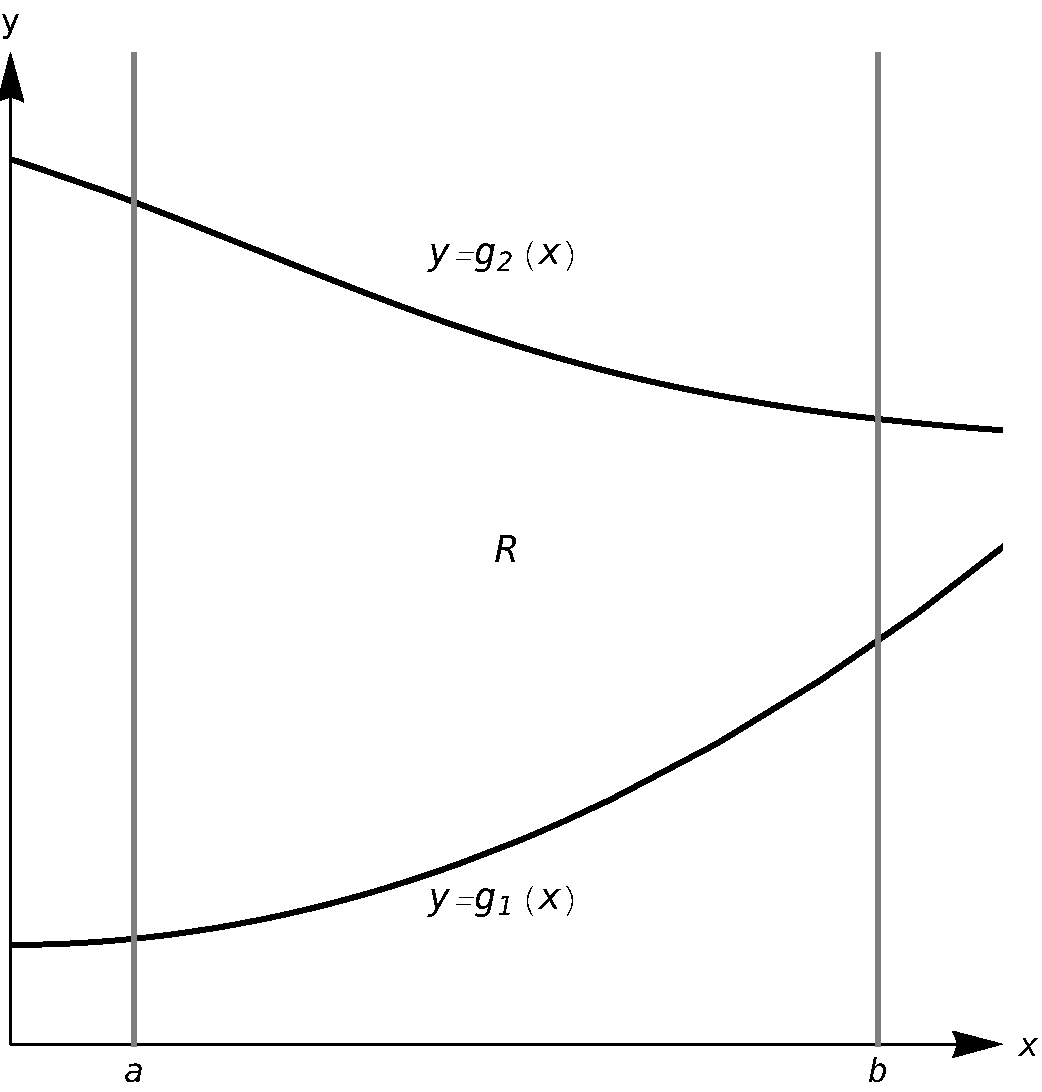
\includegraphics[width=0.43\textwidth]{fig_double_1a}}
\qquad
\subfigure[\label{fig_double_1b}]{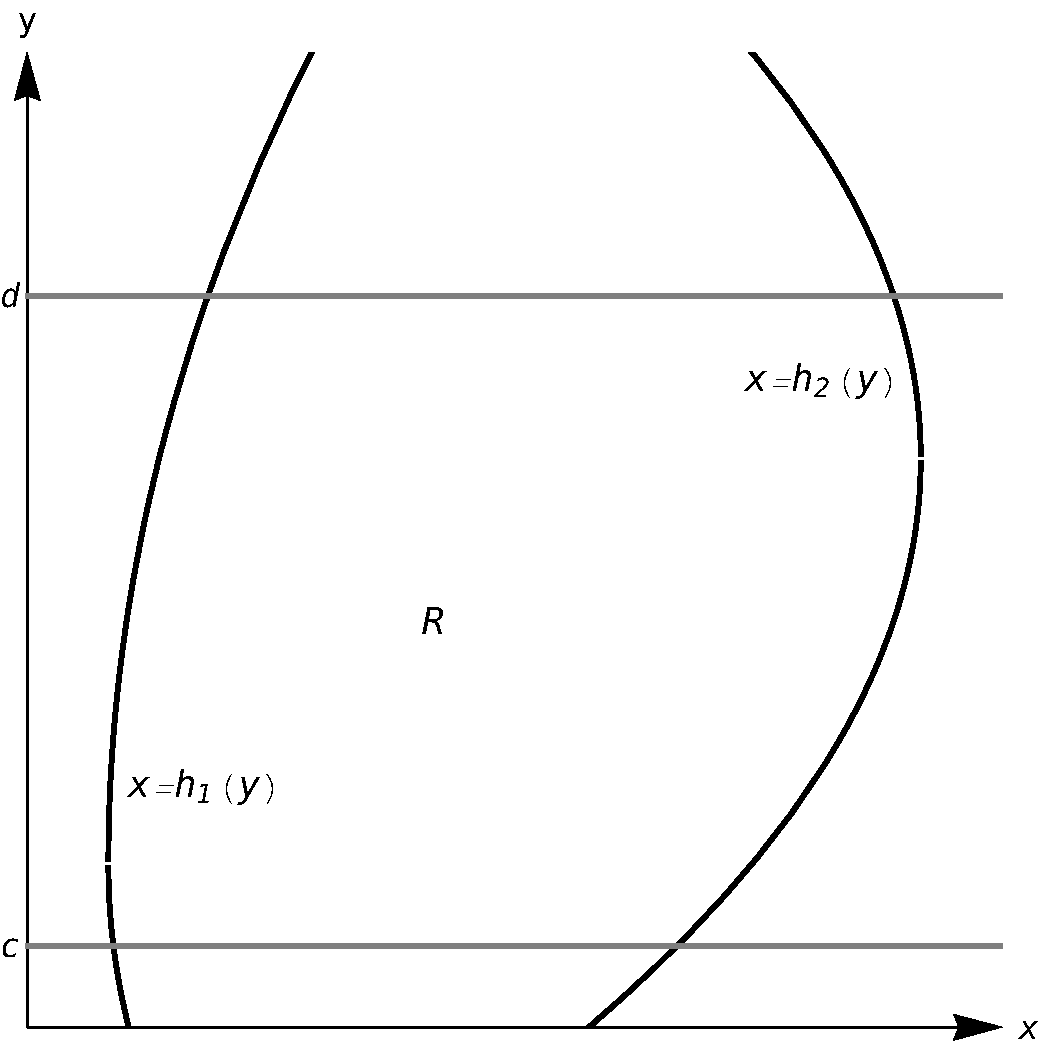
\includegraphics[width=0.43\textwidth]{fig_double_1b} }
\caption{Calculating the area of a plane region $R$ with iterated integrals. }
\end{figure}

We state this formally in a theorem.

\begin{theorem}[Area of a plane region]\label{thm:area_plane_region}
\begin{enumerate}
	\item Let $R$ be a plane region bounded by $a\leq x\leq b$ and $g_1(x)\leq y\leq g_2(x)$, where $g_1$ and $g_2$ are continuous functions on $[a,b]$. The \textbf{area $A$ of $R$} is
	$$A = \int\limits_a^b\int\limits_{g_1(x)}^{g_2(x)} \ dy\ dx.$$
	\item Let $R$ be a plane region bounded by $c\leq y\leq d$ and $h_1(y)\leq x\leq h_2(y)$, where $h_1$ and $h_2$ are continuous functions on $[c,d]$. The \textbf{area $A$ of $R$} is
	\index{integration!area}
	$$A = \int\limits_c^d\int\limits_{h_1(y)}^{h_2(y)} \ dx\ dy.$$
\end{enumerate}
\end{theorem}

The following examples should help us understand this theorem.


\begin{example}\label{ex_iterated5}
Find the area $A$ of the triangle with vertices at $(1,1)$, $(3,1)$ and $(5,5)$, as shown in Figure \ref{fig_double_2a}.



\begin{figure}[H]
\centering
%\raisebox{0.5cm}{
\subfigure[\label{fig_double_2a}]{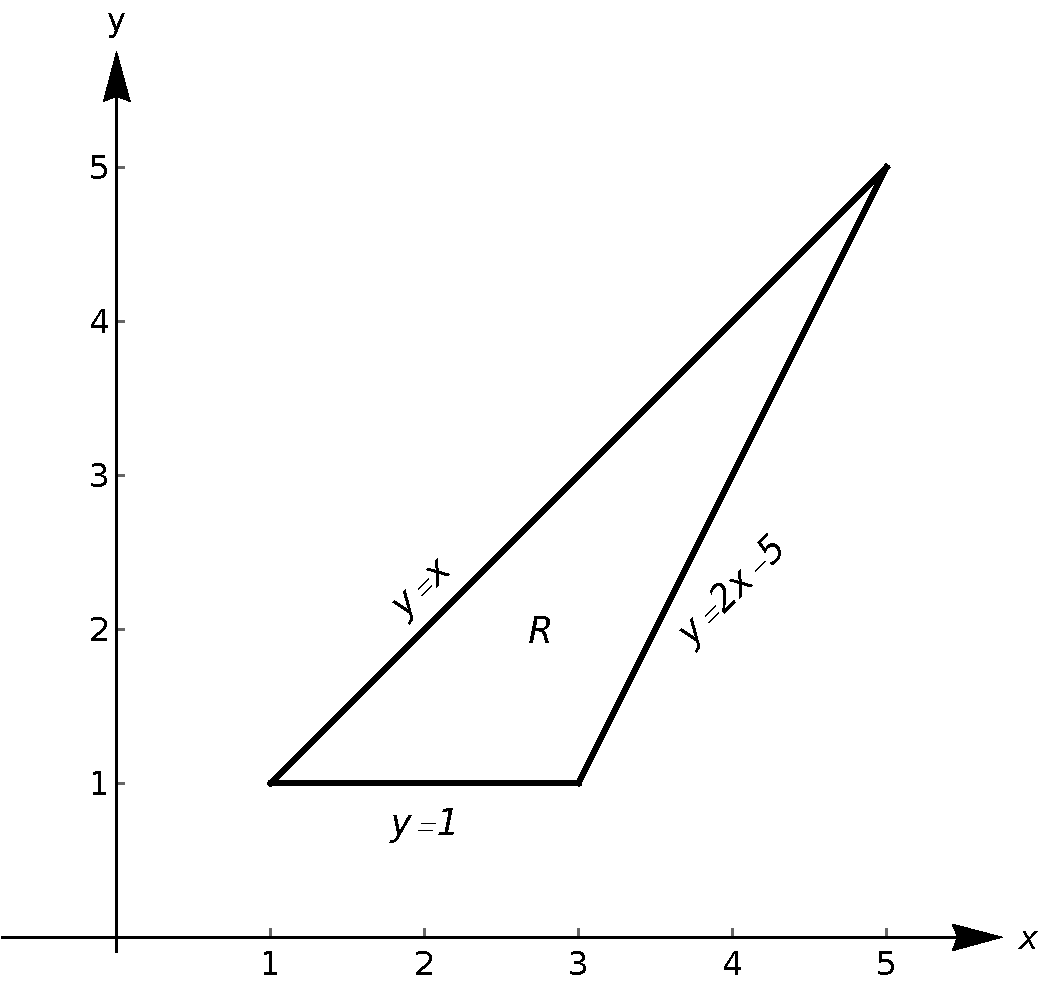
\includegraphics[width=0.4\textwidth]{fig_double_2a}}
\qquad
\subfigure[\label{fig_double_2b}]{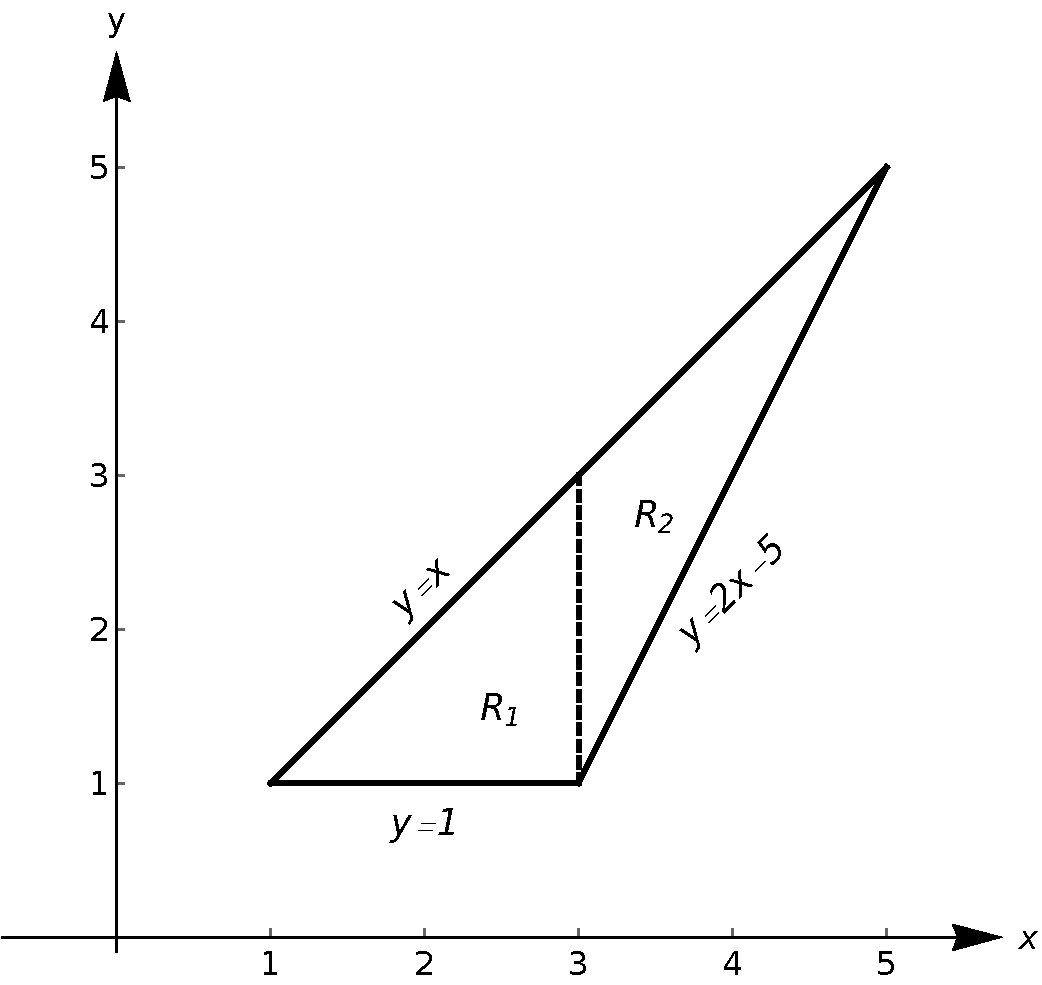
\includegraphics[width=0.4\textwidth]{fig_double_2b} }
\caption{Calculating the area of a triangle with iterated integrals in Example \ref{ex_iterated5} by using constant bounds on $y$ (a) and $x$ (b) }
\end{figure}




\xhrulefill{gray}{2.5pt}Solution \xhrulefill{gray}{2.5pt}

The triangle is bounded by the lines as shown in  Figure~\ref{fig_double_2a}. Choosing to integrate with respect to $x$ first gives that $x$ is bounded by $x=y$ to $x = \frac{y+5}2$, while $y$ is bounded by $y=1$ to $y=5$, i.e.\ the bounds with respect to $y$ are fixed. Recall that since $x$-values increase from left to right, the leftmost curve, $x=y$, is the lower bound and the rightmost curve, $x=(y+5)/2$, is the upper bound. The area is
\allowdisplaybreaks
\begin{align*}
A &= \int\limits_1^5\int\limits_{y}^{\frac{y+5}2}\ dx\ dy \\
 &= \int\limits_1^5\left(x\right)\ \Big|_y^{\frac{y+5}2}\ dy \\
&= \int\limits_1^5 \left(-\frac12y+\frac52\right)\ dy \\
&= \left(-\frac14y^2+\frac52y\right)\Bigg|_1^5\\
&=4.
\end{align*}

We can also find the area by integrating with respect to $y$ first, which implies that the bounds on $y$ are variable and dependent on $x$, whereas the one on $x$ are fixed. In this situation, though, there is not one function that defines the lower bound on the interval $[1,5]$. Essentially, we have two functions that act as the lower bound for the region $R$, $y=1$ and $y=2x-5$. In this way, the region $R$ is split into two smaller regions, namely $R_1$ and $R_2$ ( Figure~\ref{fig_double_2b}). This requires us to use two iterated integrals. Note how the $x$-bounds are different for each integral:
\begin{align*}
A &= \int\limits_1^3\int\limits_1^x 1\ dy \ dx +  \int\limits_3^5\int\limits_{2x-5}^x1\ dy\ dx\\
	&= \int\limits_1^3 y\ \Big|_1^x\ dx  + \int\limits_3^5 y \  \Big|_{2x-5}^x\ dx\\
	&= \int\limits_1^3\big(x-1\big)\ dx  +  \int\limits_3^5\big(-x+5\big)\ dx \\
	&= 2  +  2 \\
	&=4.
\end{align*}
As expected, we get the same answer both ways.
\end{example}

\begin{example}\label{ex_iterated6}
Find the area of the region enclosed by $y=2x$ and $y=x^2$, as shown in Figure \ref{fig_double_3}. 



\begin{figure}[H]
	\begin{center}
			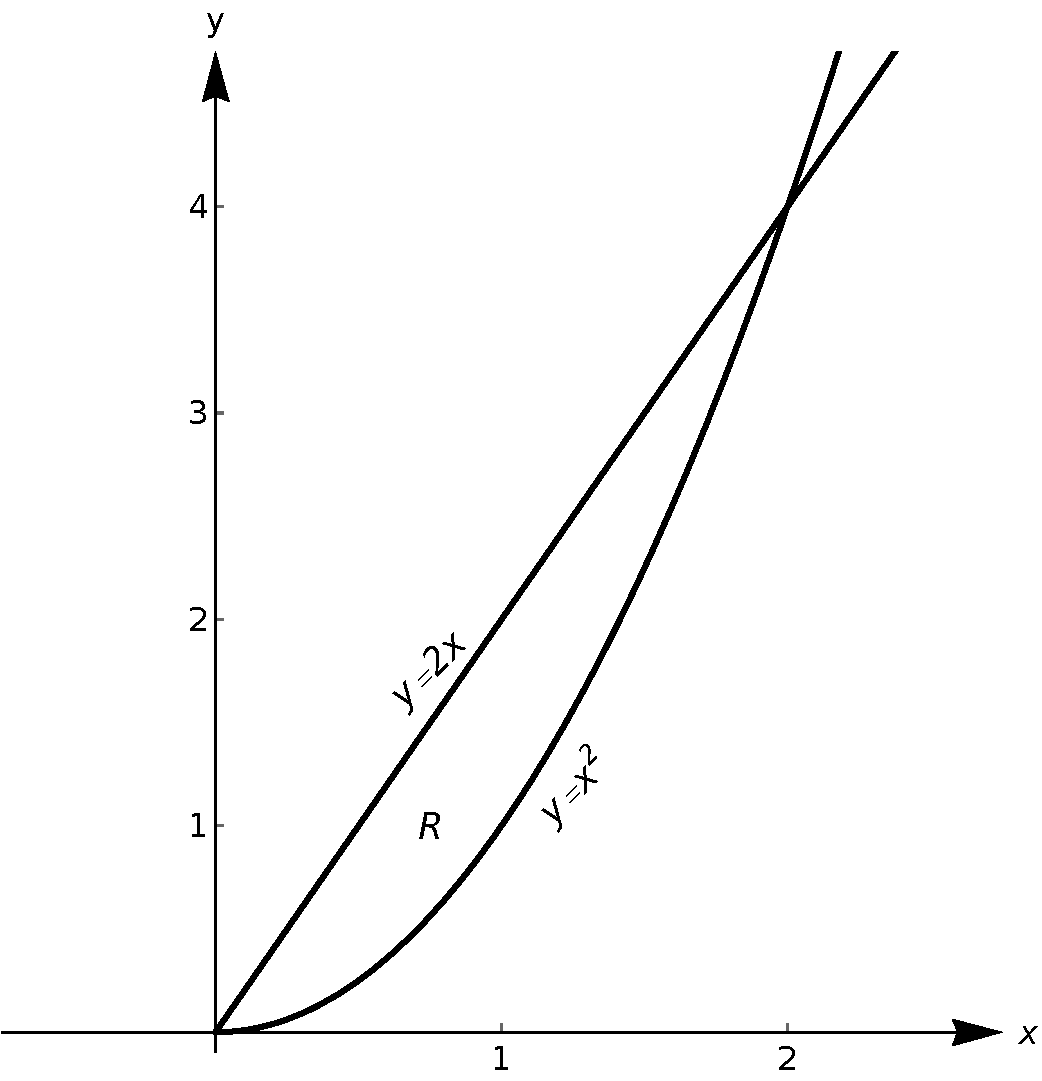
\includegraphics[width=0.4\textwidth]{fig_double_3}
	\caption{Calculating the area of a plane region with iterated integrals in Example \ref{ex_iterated6}.}
	\label{fig_double_3}
	\end{center}
\end{figure}

\xhrulefill{gray}{2.5pt}Solution \xhrulefill{gray}{2.5pt}

Once again we will find the area of the region using both orders of integration. We can approach this problem in two ways, either by choosing  fixed bounds for $x$ and variable ones - depending on $x$ - for $y$ or by choosing fixed bounds for $y$ and variable ones for $x$, which then depend on $y$. So, in the former case, we first integrate with respect to $y$ and then with respect to $x$:
$$\int\limits_0^2\int\limits_{x^2}^{2x}1\ dy \ dx = \int\limits_0^2(2x-x^2)\ dx = \left(x^2-\frac13x^3\right)\Bigg|_0^2 = \frac43.$$

In the latter case, we, however, do exactly the opposite:
$$\int\limits_0^4\int\limits_{y/2}^{\sqrt{y}} 1\ dx\ dy = \int\limits_0^4 \left(\sqrt{y}-\dfrac{y}{2} \right)\ dy = \left(\frac23y^{3/2} - \frac14y^2\right)\Big|_0^4 = \frac43.$$
\end{example}


In each of the previous examples, we have been given a region $R$ and found the bounds needed to find the area of $R$ using both orders of integration. We integrated using both orders of integration to demonstrate their equality.

We now approach the skill of describing a region using both orders of integration from a different perspective. Instead of starting with a region and creating iterated integrals, we will start with an iterated integral and rewrite it in the other integration order. To do so, we will need to understand the region over which we are integrating.

	\checkoddpage
\marginpar{\ifoddpage\hspace*{-1.5cm}\else\hspace*{0.25cm}\fi
\includegraphics[width=0.075\textwidth]{youtube}\\
\ifoddpage\hspace*{-1.75cm}\else\hspace*{0.1cm}\fi
\qrcode[height=1.75cm]{https://youtu.be/NETmfwOAKpQ}
%\includegraphics[width=0.1\textwidth]{order_int}
}

The simplest of all cases is when both integrals are bound by constants. The region described by these bounds is a rectangle, and so:
$$\int\limits_a^b\int\limits_c^d 1\ dy\ dx = \int\limits_c^d\int\limits_a^b1\ dx\ dy.$$

When the inner integral's bounds are not constants, it is generally very useful to sketch the bounds to determine what the region we are integrating over looks like. From the sketch we can then rewrite the integral with the other order of integration.

\begin{example}\label{ex_double7}
Change the order of integration of $$\ds\int\limits_0^4\int\limits_{y^2/4}^{(y+4)/2}1\ dx\ dy.$$

\xhrulefill{gray}{2.5pt}Solution \xhrulefill{gray}{2.5pt}

We sketch the region described by the bounds to help us change the integration order. $x$ is bounded below and above (i.e., to the left and right) by $x=y^2/4$ and $x=(y+4)/2$ respectively, and $y$ is bounded between 0 and 4. Graphing the previous curves, we find the region $R$ to be that shown in Figure \ref{fig_double_4a}. 


To change the order of integration, we need to give $x$ fixed bounds. The figure makes it clear that there are two lower bounds for $y$: $y=0$ on $0\leq x\leq 2$, and $y=2x-4$ on $2\leq x\leq 4$, thereby splitting $R$ in two smaller regions $R_1$ and $R_2$ (Figure \ref{fig_double_4b}). Thus we need two double integrals. The upper bound for each is $y=2\sqrt{x}$. Thus we have
$$\int\limits_0^4\int\limits_{y^2/4}^{(y+4)/2}1\ dx\ dy = \int\limits_0^2\int\limits_0^{2\sqrt{x}} 1\ dy\ dx + \int\limits_2^4\int\limits_{2x-4}^{2\sqrt{x}}1\ dy\ dx.$$



\begin{figure}[H]
\centering
%\raisebox{0.5cm}{
\subfigure[\label{fig_double_4a}]{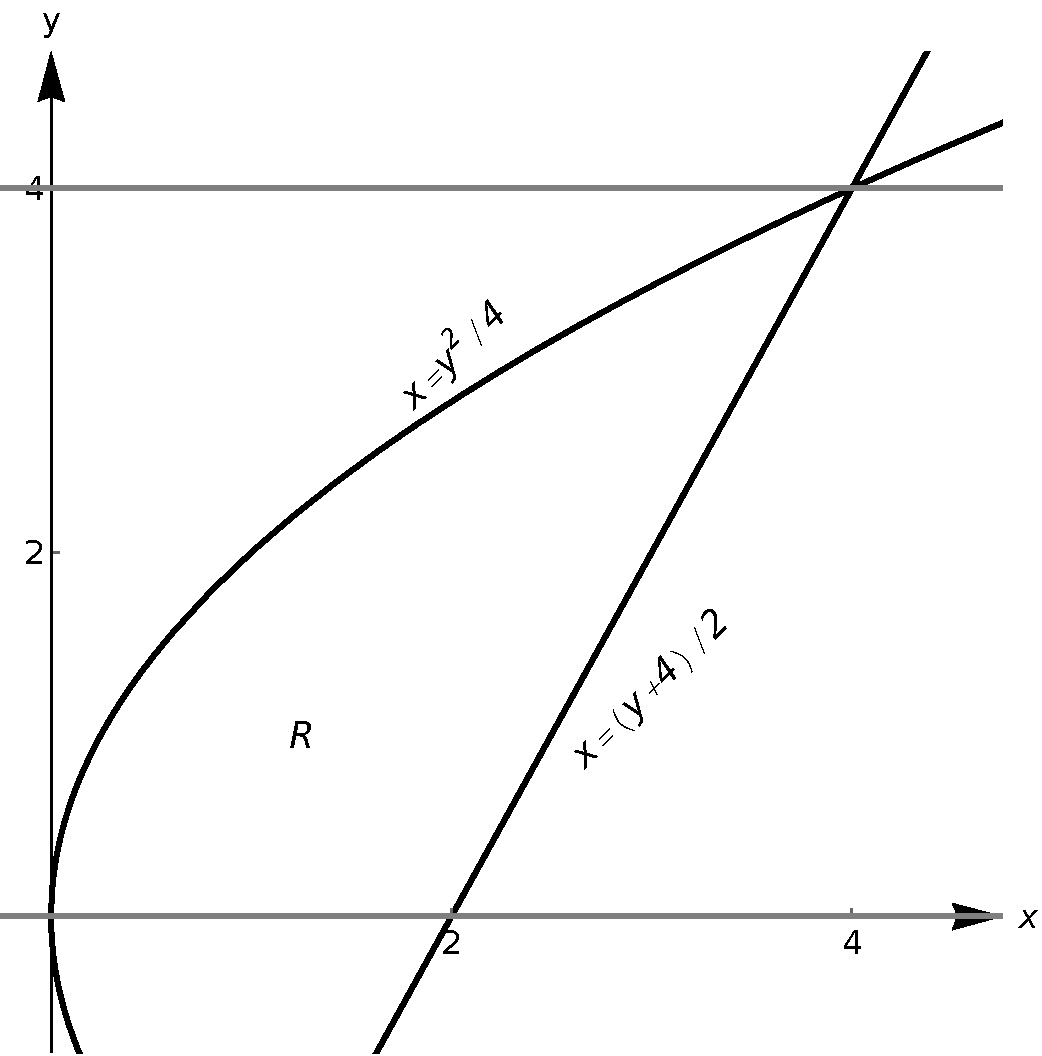
\includegraphics[width=0.4\textwidth]{fig_double_4a}}
\qquad
\subfigure[\label{fig_double_4b}]{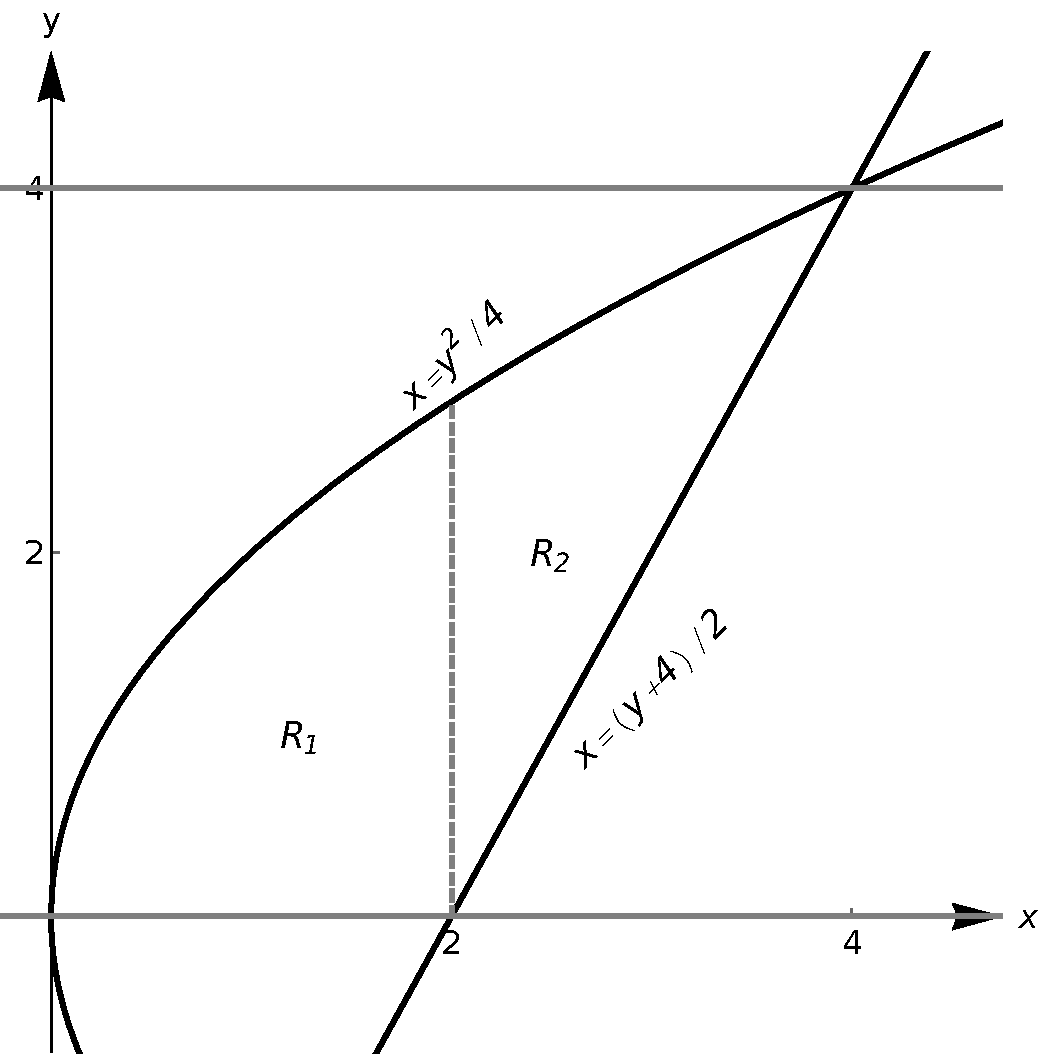
\includegraphics[width=0.4\textwidth]{fig_double_4b} }
\caption{Drawing the region determined by the bounds of integration in Example \ref{ex_double7}. }
\end{figure}


\end{example}

This section has introduced a new concept, the iterated integral. We developed one application for iterated integration: area between curves. However, this is not new, for we already know how to find areas bounded by curves. In the next section we apply iterated integration to solve problems we currently do not know how to handle. 


\section{Double integration and volume}\label{sec:double_int_volume}
\subsection{Definition}

The definite integral of $f$ over $[a,b]$, $\int\limits_a^b f(x)\ dx$, was introduced as the signed area under the curve. We approximated the value of this area by first subdividing $[a,b]$ into $n$ subintervals, where the $i^\text{ th}$ subinterval has length $\dx_i$, and letting $c_i$ be any value in the $i^\text{ th}$ subinterval. We formed rectangles that approximated part of the region under the curve with width $\dx_i$, height $f(c_i)$, and hence with area $f(c_i)\dx_i$. Summing all the rectangle's areas gave an approximation of the definite integral, and Theorem \ref{thm:riemann_sum} stated that
$$\int\limits_a^bf(x)\ dx = \lim_{\mathcal{L}\to 0}\sum f(c_i)\dx_i,$$
connecting the area under the curve with sums of the areas of rectangles.

We use a similar approach in this section to find volume under a surface. Let $R$ be a closed, bounded region in the $xy$-plane and let $z=f(x,y)$ be a continuous function defined on $R$. We wish to find the signed volume under the surface of $f$ over $R$. We use the term signed volume to denote that space above the $xy$-plane, under $f$, will have a positive volume; space above $f$ and under the $xy$-plane will have a negative volume, similar to the notion of signed area used before.

We start by partitioning $R$ into $n$ rectangular subregions as shown in Figure \ref{fig_double_5a}. For simplicity's sake, we let all widths be $\dx$ and all heights be $\dy$. Note that the sum of the areas of the rectangles is not equal to the area of $R$, but rather is a close approximation. Arbitrarily number the rectangles 1 through $n$, and pick a point $(x_i,y_i)$ in the $i^\text{ th}$ subregion. 


\begin{figure}
\centering
%\raisebox{0.5cm}{
\subfigure[\label{fig_double_5a}]{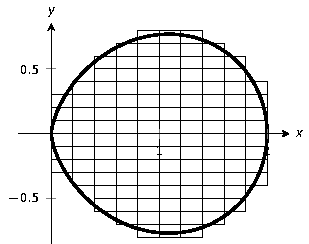
\includegraphics[width=0.43\textwidth]{fig_double_5a}}
\qquad
\subfigure[\label{fig_double_5b}]{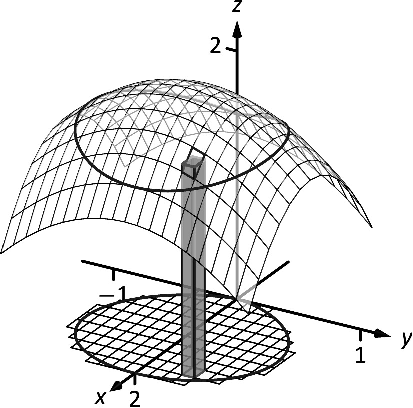
\includegraphics[width=0.43\textwidth]{fig_double_5b} }
\caption{Developing a method for finding signed volume under a surface. }
\end{figure}



The volume of the rectangular solid whose base is the $i^\text{ th}$ subregion and whose height is $f(x_i,y_i)$ is $V_i=f(x_i,y_i)\dx\dy$. Such a  solid is shown in Figure \ref{fig_double_5b}. Note how this rectangular solid only approximates the true volume under the surface; part of the solid is above the surface and part is below.

For each subregion $R_i$ used to approximate $R$, create the rectangular solid with base area $\dx\dy$ and height $f(x_i,y_i)$. 
The sum of all rectangular solids is $$\ds \sum_{i=1}^n f(x_i,y_i)\dx\dy.$$ This approximates the signed volume under $f$ over $R$. As we have done before, to get a better approximation we can use more rectangles to approximate the region $R$.

In general, each rectangle could have a different width $\dx_j$ and height $\dy_k$, giving the $i^\text{ th}$ rectangle an area $\Delta A_i = \dx_j\dy_k$ and the $i^\text{ th}$ rectangular solid a volume of $f(x_i,y_i)\Delta A_i$. Let now $\mathcal{A}$ denote the length of the longest diagonal of all rectangles in the subdivision of $R$; $\mathcal{A}\to 0$ means each rectangle's width and height are both approaching 0. If $f$ is a continuous function, as $\mathcal{A}$ shrinks (and hence $n\to +\infty$) the summation $\ds \sum_{i=1}^n f(x_i,y_i)\Delta A_i$ approximates the signed volume better and better. 

 When adding up the volumes of rectangular solids over a partition of a region $R$, as done in Figure \ref{fig_double_5b}, one could first add up the volumes across each row (one type of sum), then add these totals together (another sum), as in
$$\sum_{j=1}^n\sum_{i=1}^mf(x_i,y_j)\Delta x_i\Delta y_j.$$
One can rewrite this  as
$$\sum_{j=1}^n\left(\sum_{i=1}^mf(x_i,y_j)\Delta x_i\right)\Delta y_j.$$
The summation inside the parenthesis indicates the sum of (heights $\times$ widths), which gives an area; multiplying these areas by the thickness $\Delta y_j$ gives a volume. The illustration in Figure \ref{fig_double_5b} relates to this understanding.

This all leads us to a definition.

\begin{definition}[Double integral and signed volume]\label{def:double_int}
Let $z=f(x,y)$ be a continuous function defined over a closed, bounded region $R$ in the $xy$-plane. The \textbf{signed volume $V$ under $f$ over $R$} is denoted by the \textbf{double integral} (\textit{dubbelintegraal})
$$V = \iint_R f(x,y)\ dA.$$
\index{integration!double}\index{double integral}\index{signed volume}\index{volume}
\index[aut]{volume}\index[aut]{dubbelintegraal}
\end{definition}

Alternate notations for the double integral are

$$\iint_R f(x,y)\ dA=\iint_R f(x,y)\ dx\ dy=\iint_R f(x,y)\ dy\ dx.$$

We can find the signed volume by considering increasingly smaller, so more, rectangles; that is by considering the limit
$$\lim_{\mathcal{A}\to 0}\sum_{i=1}^n f(x_i,y_i)\Delta A_i.$$
In this limiting situation, it holds that 
\begin{equation}
V = \iint_R f(x,y)\ dA = \lim_{\mathcal{A}\to 0}\sum_{i=1}^n f(x_i,y_i)\Delta A_i.
\label{thm:double_int}
\end{equation}

Note that this equation does not specify the partition of the region $R$, so any partitioning where the diagonal of each rectangle shrinks to 0 results in the same answer. This does not offer a very satisfying way of computing volume, though. Our experience has shown that evaluating the limits of sums can be tedious. We seek a more direct method.

Recall Theorem \ref{thm:volume_by_cross_section}. This stated that if $A(x)$ gives the cross-sectional area of a solid at $x$, then $\int\limits_a^b A(x)\ dx$ gave the volume of that solid over $[a,b]$. Consider Figure \ref{fig_double_6}, where a surface $z=f(x,y)$ is drawn over a region $R$. Fixing a particular $x$-value, we can consider the area under $f$ over $R$ where $x$ has that fixed value. That area can be found with a definite integral, namely 
$$ 
A(x)=\int\limits_{g_1(x)}^{g_2(x)} f(x,y)\ dy.
$$


\begin{figure}
	\begin{center}
			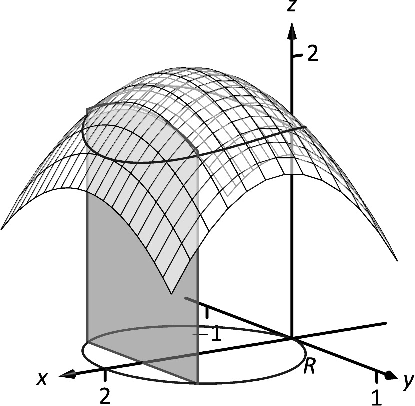
\includegraphics[width=0.5\textwidth]{fig_double_6}
	\caption{Finding volume under a surface by sweeping out a cross--sectional area.}
	\label{fig_double_6}
	\end{center}
\end{figure}

Remember that though the integrand contains $x$, we are viewing $x$ as fixed. Also note that the bounds of integration are functions of $x$: the bounds depend on the value of $x$. As $A(x)$ is a cross-sectional area function, we can find the signed volume $V$ under $f$ by integrating it:
$$V = \int\limits_a^b A(x)\ dx = \int\limits_a^b\left(\int\limits_{g_1(x)}^{g_2(x)} f(x,y)\ dy\right)dx = \int\limits_a^b\int\limits_{g_1(x)}^{g_2(x)} f(x,y)\ dy\ dx.$$

This gives a concrete method for finding signed volume under a surface. We could do a similar procedure where we started with $y$ fixed, resulting in an iterated integral with the order of integration $dx\ dy$. The following theorem states that both methods give the same result, which is the value of the double integral. It is such an important theorem it has a name associated with it.

\begin{theorem}[Fubini's theorem]\label{thm:fubini}
Let $R$ be a closed, bounded region in the $xy$-plane and let $z=f(x,y)$ be a continuous function on $R$.%
\index{double integral}\index{iterated integration}\index{signed volume}\index{volume}\index{Fubini's Theorem}\index[aut]{stelling van Fubini}
\begin{enumerate}
	\item If $R$ is bounded by $a\leq x\leq b$ and $g_1(x)\leq y\leq g_2(x)$, where $g_1$ and $g_2$ are continuous functions on $[a,b]$, then
	$$\iint_R f(x,y)\ dA = \int\limits_a^b\int\limits_{g_1(x)}^{g_2(x)} f(x,y)\ dy\ dx.$$
	
	\item If $R$ is bounded by $c\leq y\leq d$ and $h_1(y)\leq x\leq h_2(y)$, where $h_1$ and $h_2$ are continuous functions on $[c,d]$, then
	$$\iint_R f(x,y)\ dA = \int\limits_c^d\int\limits_{h_1(y)}^{h_2(y)} f(x,y)\ dx\ dy.$$
\end{enumerate}
\end{theorem}

\ifanalysis
We state this theorem without proof because it is rather technical, but it is important to realize that it is valid only if 
$$\iint_R \left|f(x,y)\right|\ dA<+\infty\,,$$
which is fulfilled if $R$ is a closed, bounded region on which $z=f(x,y)$ is a continuous function. 
\fi

\begin{example}\label{ex_double1}
Let $f(x,y) = xy+e^y$. Find the signed volume under $f$ on the region $R$, which is the rectangle with corners $(3,1)$ and $(4,2)$ pictured in Figure \ref{fig_double_7}, using both orders of integration.

\pagebreak
\xhrulefill{gray}{2.5pt}Solution \xhrulefill{gray}{2.5pt}


\begin{figure}[H]
	\begin{center}
			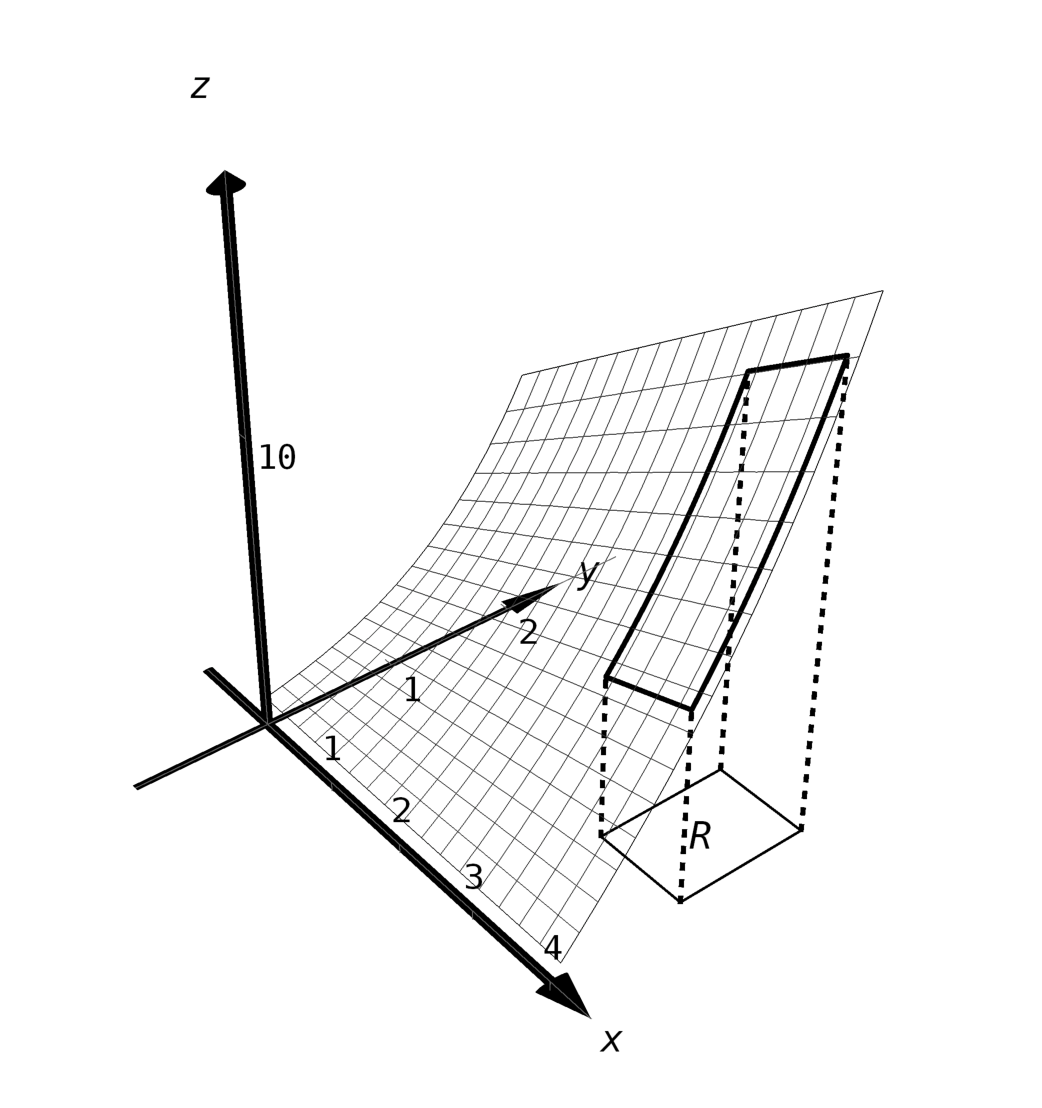
\includegraphics[width=0.55\textwidth]{fig_double_7}
	\caption{Finding the signed volume under a surface in Example \ref{ex_double1}.}
	\label{fig_double_7}
	\end{center}
\end{figure}


We wish to evaluate $\iint_R \big(xy+e^y\big)\ dA$. As $R$ is a rectangle, the bounds are easily described as $3\leq x\leq 4$ and $1\leq y\leq 2$.\\

Using the order $dy\ dx$:
\begin{align*}
\iint_R\big(xy+e^y\big) \ dA &= \int\limits_3^4\int\limits_1^2\big(xy+e^y\big)\ dy \ dx \\
			&= \int\limits_3^4 \left.\left(\frac12xy^2+e^y\right)\right|_1^2\  dx \\
			&= \int\limits_3^4\left(\frac 32x + e^2-e\right)\ dx \\
			&= \left.\left(\frac 34x^2 + \big(e^2-e\big)x\right)\right|_3^4 \\
			&= \frac {21}4+ e^2-e\approx 9.92.
\end{align*}


Now we check the validity of Fubini's theorem by using the order $dx\ dy$:
\allowdisplaybreaks
\begin{align*}
\iint_R\big(xy+e^y\big) \ dA &= \int\limits_1^2\int\limits_3^4\big(xy+e^y\big)\ dx \ dy \\
		&= \int\limits_1^2\left.\left(\frac12x^2y+xe^y\right)\right|_3^4\ dy\\
		&= \int\limits_1^2\left(\frac72y+e^y\right)\ dy\\
		&= \left.\left(\frac74y^2+e^y\right)\right|_1^2\\
		&=\frac{21}4+e^2-e\approx 9.92.
\end{align*}
Both orders of integration return the same result, as expected.
\end{example}


\begin{example}\label{ex_double2}
Evaluate $$\iint_R \big(3xy-x^2-y^2+6\big)\ dA,$$
where $R$ is the triangle bounded by $x=0$, $y=0$ and  $x/2+y=1$, as shown in Figure \ref{fig_double_8}.

\begin{figure}[H]
	\begin{center}
			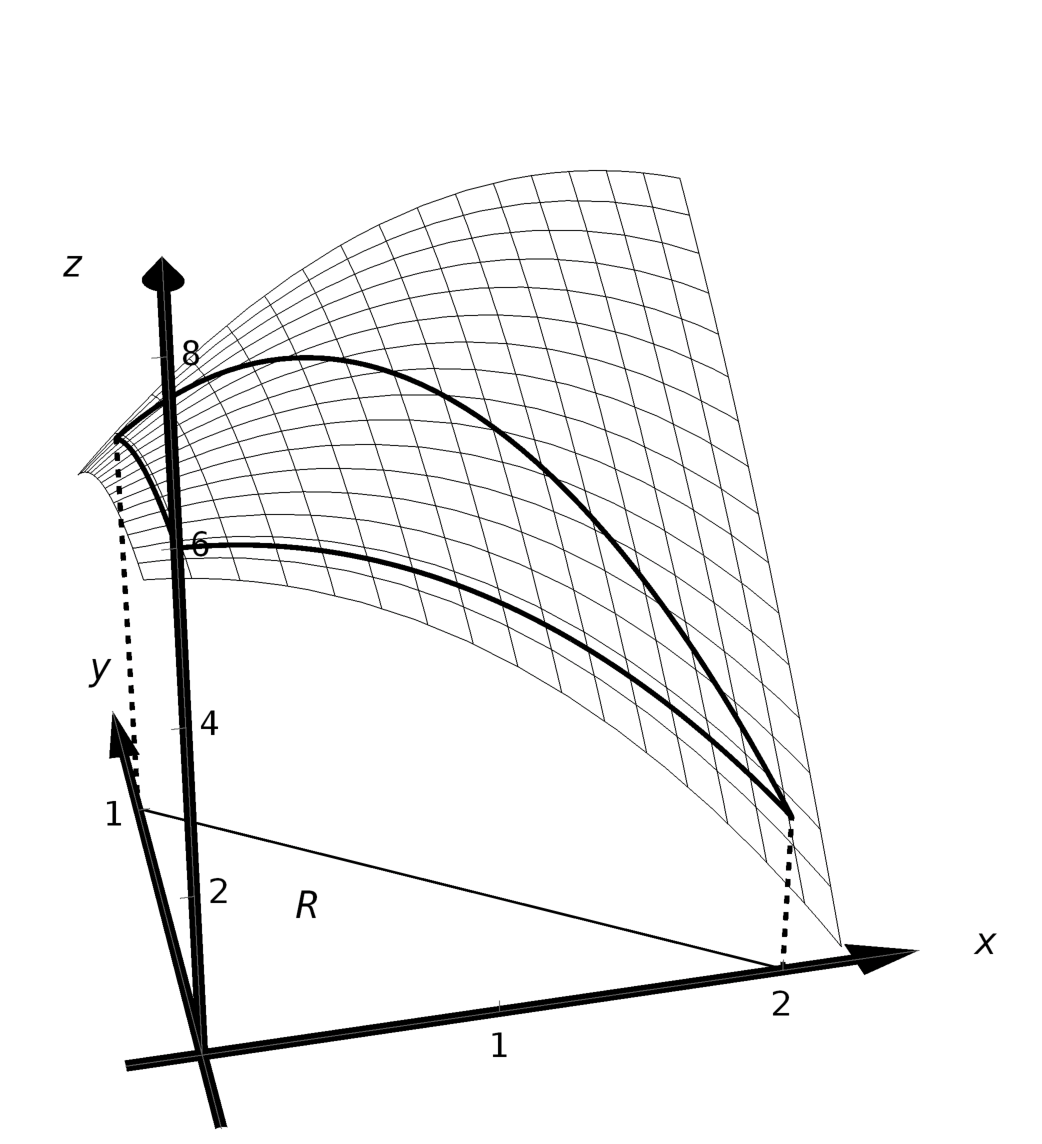
\includegraphics[width=0.5\textwidth]{fig_double_8}
	\caption{Finding the signed volume under a surface in Example \ref{ex_double2}.}
	\label{fig_double_8}
	\end{center}
\end{figure}


\xhrulefill{gray}{2.5pt}Solution \xhrulefill{gray}{2.5pt}

While it is not specified which order we are to use, we will evaluate the double integral using both orders to help drive home the point that it does not matter which order we use.\\


Using the order $dy\ dx$:
The bounds on $y$ go from curve to curve, i.e., $0\leq y\leq 1-x/2$, and the bounds on $x$ go from point to point, i.e., $0\leq x\leq 2$.
\allowdisplaybreaks
\begin{align*}
\iint_R (3xy-x^2-y^2+6\big)\ dA &= \int\limits_0^2\int\limits_0^{-\frac x2+1} (3xy-x^2-y^2+6\big)\ dy\ dx\\
		&= \int\limits_0^2 \left.\left(\frac32xy^2-x^2y-\frac13y^3+6y\right)\right|_0^{-\frac x2+1} dx\\
		&= \int\limits_0^2 \left(\frac{11}{12}x^3-\frac{11}{4}x^2-x+\frac{17}3\right)\ dx \\
		&= \left.\left(\frac{11}{48}x^4-\frac{11}{12}x^3-\frac12x^2+\frac{17}3x\right)\right|_0^2\\
		&= \frac{17}3\approx5.6.
\end{align*}

Now lets consider the order $dx \ dy$. Here $x$ goes from curve to curve, $0\leq x\leq 2-2y$, and $y$ goes from point to point, $0\leq y\leq 1$:
\begin{align*}
\iint_R (3xy-x^2-y^2+6\big)\ dA &= \int\limits_0^1\int\limits_0^{2-2y} (3xy-x^2-y^2+6\big)\ dx\ dy\\
		&= \int\limits_0^1 \left.\left(\frac32x^2y-\frac13x^3-xy^2+6x\right) \right|_0^{2-2y} dy\\
		&= \int\limits_0^1\left(\frac{32}3y^3-22y^2+2y+\frac{28}3\right)\ dy\\
		&=\left.\left(\frac83y^4-\frac{22}3y^3+y^2+\frac{28}3y\right)\right|_0^1\\
		&=\frac{17}3\approx5.6.
\end{align*}
We obtained the same result using both orders of integration. 
\end{example}

\subsection{Properties}

Note how in these two examples that the bounds of integration depend only on $R$; the bounds of integration have nothing to do with $f(x,y)$. Moreover, let $f$ and $g$ be continuous functions over a closed, bounded plane region $R$, and let $c$ be a constant, then we have the following properties, in line with the ones of single integrals. 

\begin{itemize}
	\item Constant multiple rule:
	$$\ds \iint_Rc\,f(x,y)\ dA = c\iint_Rf(x,y)\ dA.$$
	\item Sum/Difference rule:	
	$$\ds \iint_R \big(f(x,y)\pm g(x,y)\big)\ dA = \iint_R f(x,y)\ dA \pm \iint_R g(x,y)\ dA $$
	\item	If $f(x,y)\geq 0$ on $R$, then $$\ds \iint_R f(x,y)\ dA\geq 0.$$
	\item	If $f(x,y)\geq g(x,y)$ on $R$, then $$\ds \iint_R f(x,y)\ dA\geq \iint_R g(x,y)\ dA.$$
	\item Let $R$ be the union of two nonoverlapping regions, $R = R_1\cup R_2$. Then 
	$$\iint_R f(x,y)\ dA = \iint_{R_1}f(x,y)\ dA+ \iint_{R_2}f(x,y)\ dA.$$
\end{itemize}
Actually, since this property is intuitively clear, we relied already in Examples~\ref{ex_iterated5} and \ref{ex_double7}. Of course, this property generalizes to $n$ nonoverlapping regions.


\begin{example}\label{ex_double3}
Let $f(x,y) = \sin(x)\cos(y)$ and $R$ be the triangle with vertices $(-1,0)$, $(1,0)$ and $(0,1)$ (see Figure \ref{fig_double_9}). Evaluate the double integral $\iint_Rf(x,y)\ dA$.

\begin{figure}[H]
	\begin{center}
			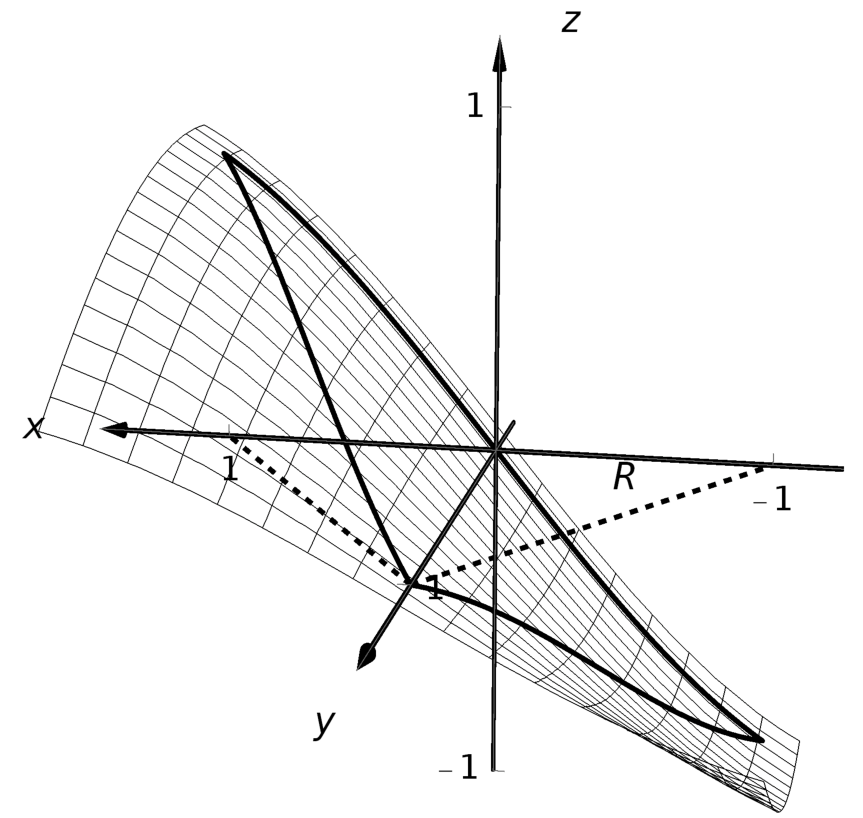
\includegraphics[width=0.5\textwidth]{fig_double_9}
	\caption{Finding the signed volume under a surface in Example \ref{ex_double3}.}
	\label{fig_double_9}
	\end{center}
\end{figure}


\xhrulefill{gray}{2.5pt}Solution \xhrulefill{gray}{2.5pt}


If we attempt to integrate using an iterated integral with the order $dy\ dx$, note how there are two upper bounds on $R$ meaning we will need to use two iterated integrals. We would need to split the triangle into two regions along the $y$-axis.

Instead, let us use the order $dx\ dy$. The curves bounding $x$ are $y-1\leq x\leq 1-y$; the bounds on $y$ are $0\leq y\leq 1$. This gives us:
\allowdisplaybreaks
\begin{align*}
\iint_R f(x,y)\ dA &= \int\limits_0^1\int\limits_{y-1}^{1-y}\sin(x)\cos(y)\ dx\ dy\\
		&= \int\limits_0^1\left.\Big( -\cos(x)\cos(y)\Big)\right|_{y-1}^{1-y} dy\\
		&= \int\limits_0^1 \cos(y)\Big(-\cos(1-y) + \cos(y-1)\Big)\ dy.
\end{align*}
Recall that the cosine function is an even function; that is, $\cos(x) = \cos(-x)$. Therefore, from the last integral above, we have $\cos(y-1) = \cos(1-y)$. Thus the integrand simplifies to 0, and we have 
$$
\iint_R f(x,y)\ dA = \int\limits_0^1 0\ dy = 0.
$$
It turns out that over $R$, there is just as much volume above the $xy$-plane as below (look again at Figure \ref{fig_double_9}), giving a final signed volume of 0. 
\end{example}

In the previous section we practised changing the order of integration of a given iterated integral, where the region $R$ was not explicitly given. Changing the bounds of an integral is more than just an test of understanding. Rather, there are cases where integrating in one order is really hard, if not impossible, whereas integrating with the other order is feasible.

\begin{example}\label{ex_double6}
Rewrite the iterated integral 
$$\ds \int\limits_0^3\int\limits_y^3 e^{-x^2}\ dx\ dy$$
with the order $dy\ dx$. Comment on the feasibility to evaluate each integral.

\xhrulefill{gray}{2.5pt}Solution \xhrulefill{gray}{2.5pt}

Once again we make a sketch of the region over which we are integrating to facilitate changing the order. The bounds on $x$ are from $x=y$ to $x=3$; the bounds on $y$ are from $y=0$ to $y=3$. These curves are sketched in Figure \ref{fig_double_10a}, enclosing the region $R$.

To change the bounds, note that the curves bounding $y$ are $y=0$ up to $y=x$; the triangle is enclosed between $x=0$ and $x=3$. Thus the new bounds of integration are $0\leq y\leq x$ and $0\leq x\leq 3$, giving the iterated integral $$\ds \int\limits_0^3\int\limits_0^x e^{-x^2}\ dy\ dx.$$ How easy is it to evaluate each iterated integral? Consider the order of integrating $dx\ dy$, as given in the original problem. The first indefinite integral we need to evaluate is $\int\limits e^{-x^2}\ dx$; we have stated before  that this integral cannot be evaluated in terms of elementary functions. We are stuck.

Changing the order of integration makes a big difference here. In the second iterated integral, we are faced with $\int\limits e^{-x^2}\ dy$; integrating with respect to $y$ gives us $ye^{-x^2}+C$, and the first definite integral evaluates to 
$$\int\limits_0^x e^{-x^2}\ dy = xe^{-x^2}.$$
Thus 
$$\int\limits_0^3\int\limits_0^x e^{-x^2}\ dy\ dx = \int\limits_0^3 xe^{-x^2}\ dx.$$
This last integral is easy to evaluate with substitution, giving a final answer of $(1-e^{-9})/2\approx 0.5$. Figure \ref{fig_double_10b} shows the surface over $R$. In short, evaluating one iterated integral is impossible; the other iterated integral is relatively simple.

\begin{figure}[H]
\centering
%\raisebox{0.5cm}{
\subfigure[\label{fig_double_10a}]{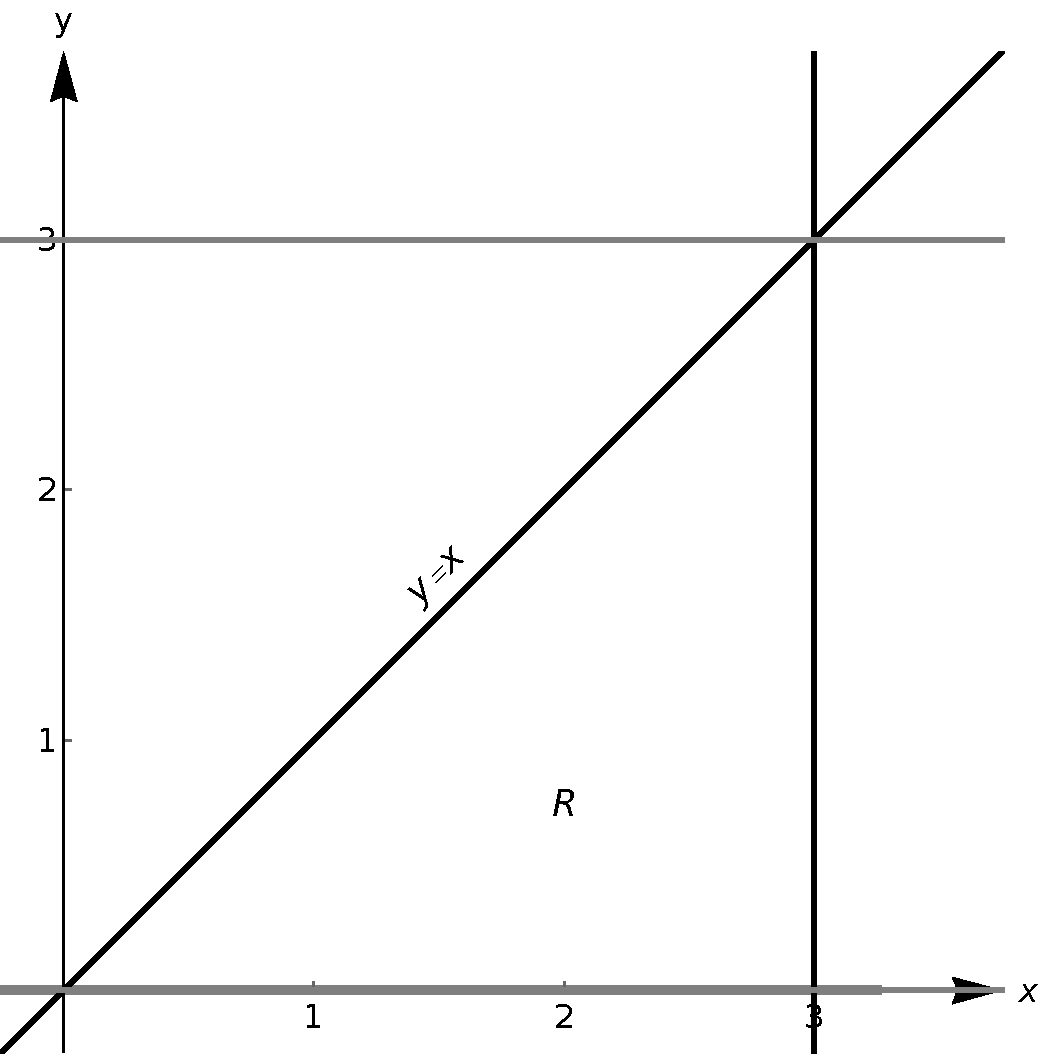
\includegraphics[width=0.43\textwidth]{fig_double_10a}}
\qquad
\subfigure[\label{fig_double_10b}]{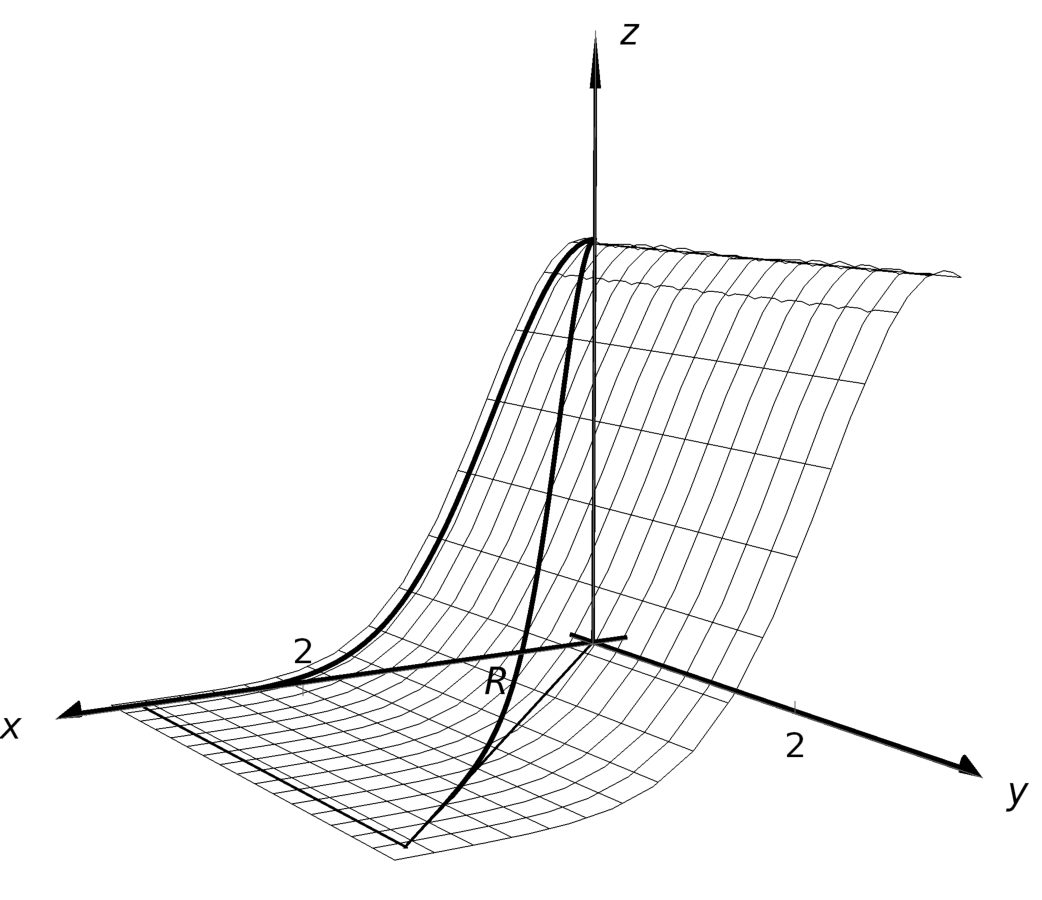
\includegraphics[width=0.43\textwidth]{fig_double_10b} }
\caption{Determining the region $R$ determined by the bounds of integration (a) and the surface $f$ over its region $R$ in Example \ref{ex_double6}.}
\end{figure}

\end{example}

	\checkoddpage
\marginpar{\ifoddpage\hspace*{-1.5cm}\else\hspace*{0.25cm}\fi
\includegraphics[width=0.075\textwidth]{youtube}\\
\ifoddpage\hspace*{-1.75cm}\else\hspace*{0.1cm}\fi
\qrcode[height=1.75cm]{https://youtu.be/dzuoNwC6Ze}
%\includegraphics[width=0.1\textwidth]{mean_function_value_3d}
}

Using double integrals we can also determine the average value of $z=f(x,y)$ over a region $R$. This is nothing but the volume under $f$ over $R$ divided by the area of $R$; that is
\begin{equation}
\text{average value of $f$ on $R$} = \frac{\ds \iint_R f(x,y)\ dA}{\ds\iint_R \ dA}.
\label{def:av_val2}
\end{equation}


\begin{example}\label{ex_double8}
Find the average value of $f(x,y) = 4-y$ over the region $R$, which is bounded by the parabolas $y^2=4x$ and $x^2=4y$ (see Figure~\ref{fig_double_11}). 




\xhrulefill{gray}{2.5pt}Solution \xhrulefill{gray}{2.5pt}

Graphing each curve can help us find their points of intersection. Solving analytically, the second equation tells us that $y=x^2/4$. Substituting this value in for $y$ in the first equation gives us $x^4/16 = 4x$. Solving for $x$:

\allowdisplaybreaks
\begin{align*}
& \qquad \frac{x^4}{16} = 4x\\
\Leftrightarrow & \qquad x^4-64x = 0\\
\Leftrightarrow & \qquad x(x^3-64)  = 0\\
\Leftrightarrow & \qquad x = 0 \;  \vee \;  x = 4.
\end{align*}
Thus we have found analytically what was easy to approximate graphically: the regions intersect at $(0,0)$ and $(4,4)$, as shown in Figure \ref{fig_double_11}. 



We now choose an order of integration: $dy\ dx$ or $dx\ dy$? Either order works; since the integrand does not contain $x$, choosing $dx\ dy$ might be simpler -- at least, the first integral is very simple.

Thus we have the following curve to curve, point to point bounds: $y^2/4\leq x\leq 2\sqrt y$, and $0\leq y\leq 4$. 
\begin{align*}
\iint_R (4-y)\ dA &= \int\limits_0^4\int\limits_{y^2/4}^{2\sqrt{y}}(4-y)\ dx\ dy\\
&= \int\limits_0^4(4-y)\int\limits_{y^2/4}^{2\sqrt{y}}\ dx\ dy\\
				&= \int\limits_0^4 \big(x(4-y)\big)\Big|_{y^2/4}^{2\sqrt{y}} dy\\
				&= \int\limits_0^4 \left[\left(2\sqrt{y}-\frac{y^2}{4}\right)(4-y)\right]\ dy = \int\limits_0^4 \Big( \frac{y^3}{4}-y^2-2y^{3/2}+8y^{1/2}\Big)\ dy\\
				&= \left.\left(\frac{y^4}{16}-\frac{y^3}{3}-\frac{4y^{5/2}}5+\frac{16y^{3/2}}3\right)\right|_0^4\\
				&= \frac{176}{15} \approx 11.73.
\end{align*}



We now find the area of $R$ by computing $\iint_R \ dA$:
$$\iint_R \ dA = \int\limits_0^4\int\limits_{y^2/4}^{2\sqrt{y}} \ dx\ dy = \frac{16}{3}.$$
Dividing the volume under the surface by the area gives the average value:
$$\text{average value of $f$ on $R$} = \frac{176/15}{16/3} = \frac{11}5 = 2.2.$$
While the surface covers $z$-values from $z=0$ to $z=4$, the average $z$-value on $R$ is 2.2.

\begin{figure}[H]
	\begin{center}
			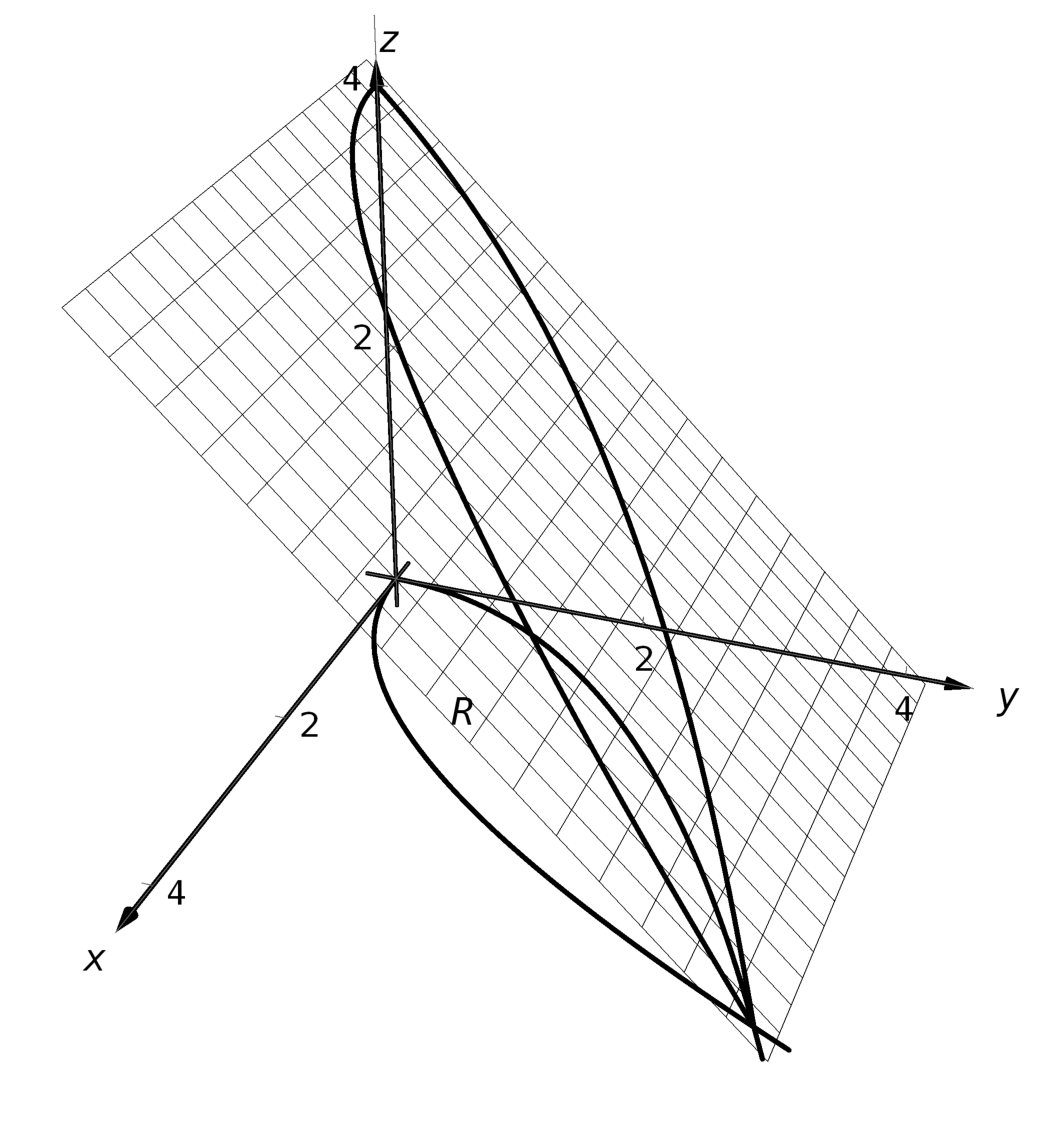
\includegraphics[width=0.5\textwidth]{fig_double_11}
	\caption{Finding the signed volume under a surface in Example \ref{ex_double8}.}
	\label{fig_double_11}
	\end{center}
\end{figure}
\end{example}

Our new understanding of double integrals allows us to revisit what we did in the previous section. Given a region $R$ in the plane, we computed $\iint_R 1\ dA$; again. Our understanding at the time was that we were finding the area of $R$. However, we can now view the function $z=1$ as a surface, a flat surface with constant $z$-value of 1. The double integral $\iint_R 1\ dA$ finds the volume, under $z=1$, over $R$. We were actually computing the volume of a solid, though we interpreted the number as an area.




\subsection{Double integration with polar coordinates}
\label{sec:double_int_polar}
Some regions $R$ are easy to describe using rectangular coordinates -- that is, with equations of the form $y=f(x)$, $x=a$, etc. However, some regions are easier to handle if we represent their boundaries with polar equations of the form $r=f(\theta)$, $\theta = \alpha$, etc. 

The basic form of the double integral is $\iint_R f(x,y)\ dA$. We interpret this integral as follows: over the region $R$, sum up lots of products of heights (given by $f(x_i,y_i)$) and areas (given by $\Delta A_i$). That is, $dA$ represents a little bit of area. In rectangular coordinates, we can describe a small rectangle as having area $dx\ dy$ or $dy\ dx$ -- the area of a rectangle is simply (length$\times$width) -- a small change in $x$ times a small change in $y$. Thus we replace $dA$ in the double integral with $dx\ dy$ or $dy\ dx$.

Now consider representing a region $R$ with polar coordinates. Consider Figure \ref{fig_double_12a}. Let $R$ be the region in the first quadrant bounded by the curve. We can approximate this region using the natural shape of polar coordinates: portions of sectors of circles. In the figure, one such region is shaded, shown again in Figure~\ref{fig_double_12b}.

\begin{figure}
\centering
%\raisebox{0.5cm}{
\subfigure[\label{fig_double_12a}]{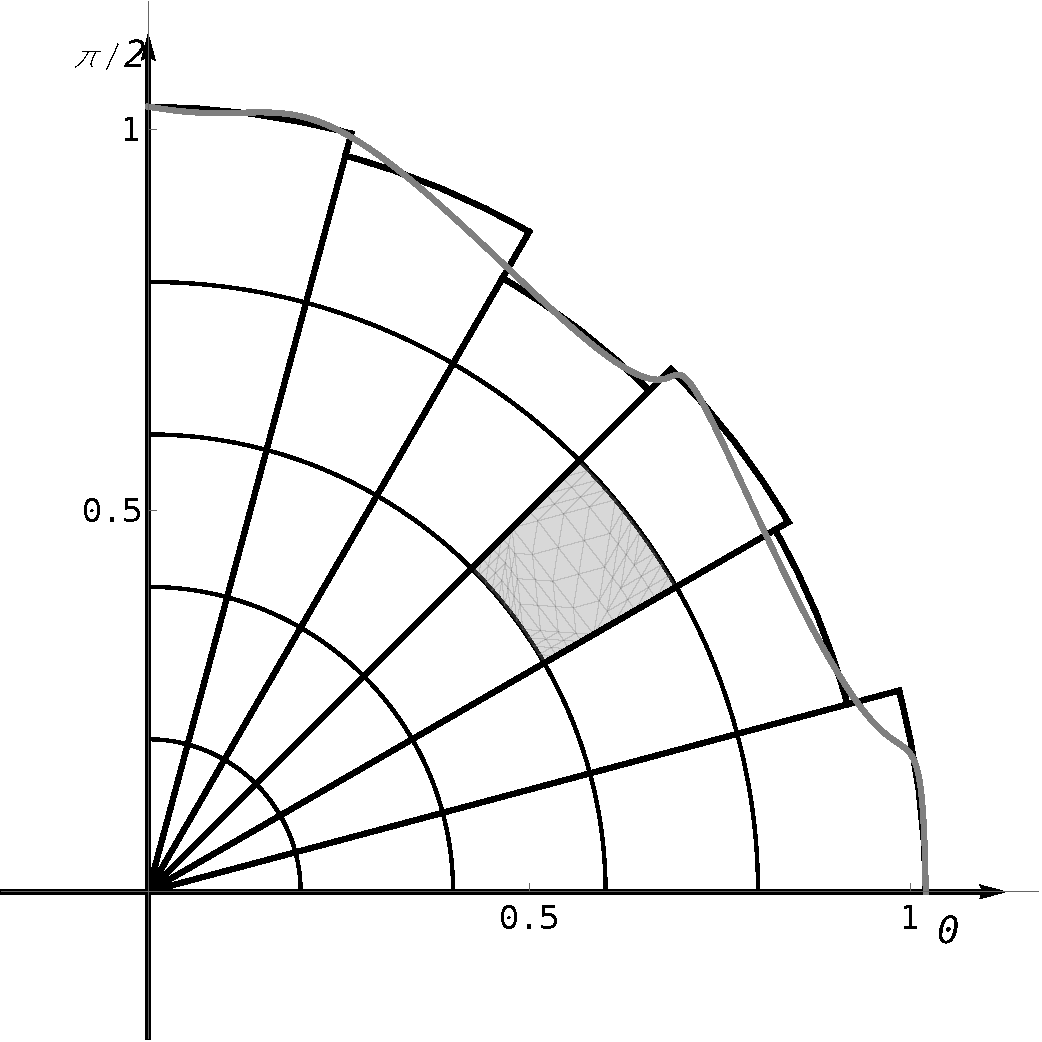
\includegraphics[width=0.43\textwidth]{fig_double_12a}}
\qquad
\subfigure[\label{fig_double_12b}]{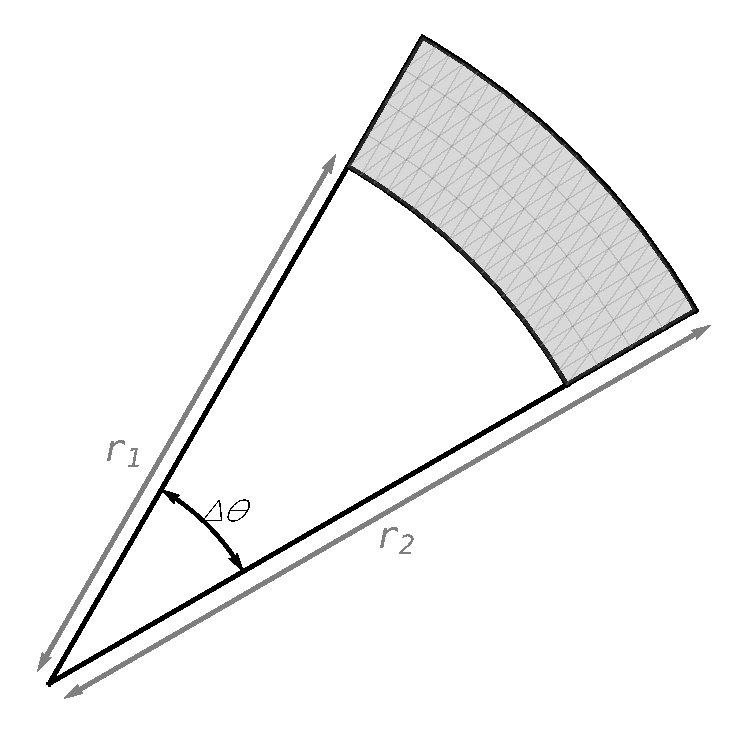
\includegraphics[width=0.43\textwidth]{fig_double_12b} }
\caption{Approximating a region $R$ with portions of sectors of circles.}
\end{figure}

As the area of a sector of a circle with radius $r$, subtended by an angle $\theta$, is $A = \frac12r^2\theta$, we can find the area of the shaded region. The whole sector has area $\frac12r_2^2\Delta \theta$, whereas the smaller, unshaded sector has area $\frac12r_1^2\Delta \theta$. The area of the shaded region is the difference of these areas:
$$\Delta A_i = \frac12r_2^2\Delta\theta-\frac12r_1^2\Delta\theta = \frac12\big(r_2^2-r_1^2\big) \Delta\theta = \frac{r_2+r_1}{2}\big(r_2-r_1\big) \Delta\theta.$$

Note that $(r_2+r_1)/2$ is just the average of the two radii. 

To approximate the region $R$, we use many such subregions; doing so shrinks the difference $r_2-r_1$ between radii to 0 and shrinks the change in angle $\Delta \theta$ also to 0. We represent these infinitesimal changes in radius and angle as $dr$ and $d\theta$, respectively. Finally, as $dr$ is small, $r_2\approx r_1$, and so \\ $(r_2+r_1)/2\approx r_1$. Thus, when $dr$ and $d\theta$ are small, 
$$\Delta A_i \approx r_i\ dr\ d\theta.$$

Taking a limit, where the number of subregions goes to infinity and both $r_2-r_1$ and $\Delta\theta$ go to 0, we get $$dA = r\ dr\ d\theta.$$

So to evaluate $\iint_Rf(x,y)\ dA$, replace $dA$ with $r\ dr\ d\theta$. Convert the function $z=f(x,y)$ to a function with polar coordinates with the substitutions $x=r\cos(\theta)$, $y=r\sin(\theta)$. Finally, find bounds $g_1(\theta)\leq r\leq g_2(\theta)$ and $\alpha\leq\theta\leq\beta$ that describe $R$. Consequently, if $z=f(x,y)$ is a continuous function defined over a closed, bounded region $R$ in the $xy$-plane, where $R$ is
%Let $R$ be a plane region 
bounded by the polar equations $\alpha\leq\theta\leq\beta$ and  $g_1(\theta)\leq r\leq g_2(\theta)$, then 
\begin{equation}
\iint_Rf(x,y)\ dA = \int\limits_\alpha^\beta\int\limits_{g_1(\theta)}^{g_2(\theta)} f\big(r\cos(\theta),r\sin(\theta)\big)\ r\ dr\ d\theta.
\label{idea:doublepol}
\end{equation}

Examples will help us understand this.

\begin{example}\label{ex_doublepol1}
Find the signed volume under the plane $z= 4-x-2y$ over the disk bounded by the circle with equation $x^2+y^2=1$.

\xhrulefill{gray}{2.5pt}Solution \xhrulefill{gray}{2.5pt}

The bounds of the integral are determined solely by the region $R$ over which we are integrating. In this case, it is a disk with boundary $x^2+y^2=1$. We need to find polar bounds for this region. Bounds for this disk are $0\leq r\leq 1$ and $0\leq \theta\leq 2\pi$.

We replace $f(x,y)$ with $f\left(r\cos(\theta),r\sin(\theta)\right)$. That means we make the following substitutions:
$$4-x-2y \quad \Rightarrow \quad 4-r\cos(\theta)-2r\sin(\theta).$$
Finally, we replace $dA$ in the double integral with $r\ dr\ d\theta$. This gives the final iterated integral, which we evaluate:
\allowdisplaybreaks
\begin{align*}
\iint_Rf(x,y)\ dA &= \int\limits_0^{2\pi}\int\limits_0^1\big(4-r\cos(\theta)-2r\sin(\theta)\big)r\ dr\ d\theta\\
						&= \int\limits_0^{2\pi}\int\limits_0^1\Big(4r-r^2\big(\cos(\theta)-2\sin(\theta)\big)\Big)\ dr\ d\theta\\
						&= \int\limits_0^{2\pi}\left.\left(2r^2-\frac13r^3\big(\cos(\theta)-2\sin(\theta)\big)\right)\right|_0^1d\theta\\
						&= \int\limits_0^{2\pi} \left(2-\frac13\big(\cos(\theta)-2\sin(\theta)\big)\right)\ d\theta\\
						&= \left.\left(2\theta -\frac13\big(\sin(\theta)+2\cos(\theta)\big)\right)\right|_0^{2\pi} \\
						&= 4\pi \approx 12.566.
\end{align*}
The surface and region $R$ are shown in Figure \ref{fig_double_13}.

\begin{figure}[H]
	\begin{center}
			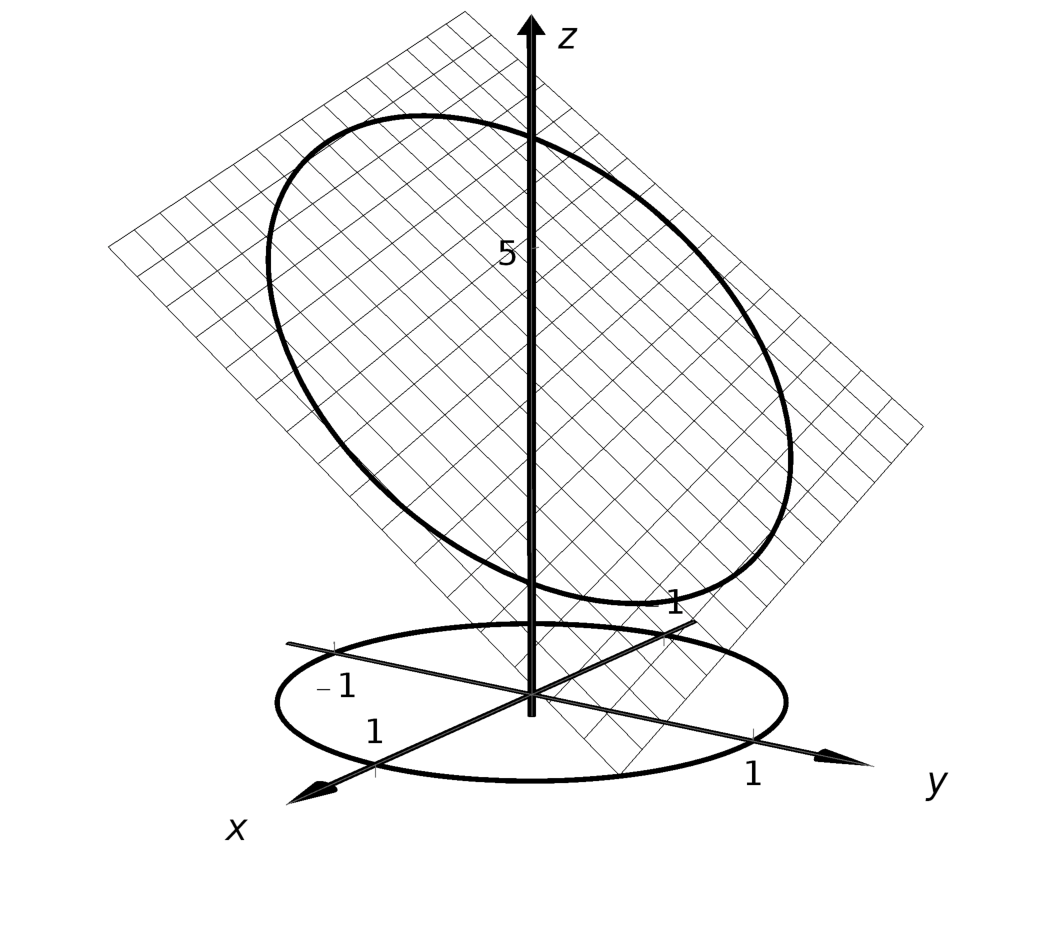
\includegraphics[width=0.4\textwidth]{fig_double_13}
	\caption{Evaluating a double integral with polar coordinates in Example \ref{ex_doublepol1}.}
	\label{fig_double_13}
	\end{center}
\end{figure}

\end{example}

\begin{example}\label{ex_doublepol2}
Find the volume under the paraboloid $z=4-(x-2)^2-y^2$ over the region bounded by the circles $(x-1)^2+y^2=1$ and $(x-2)^2+y^2=4$.

\pagebreak
\xhrulefill{gray}{2.5pt}Solution \xhrulefill{gray}{2.5pt}

At first glance, this seems like a very hard volume to compute as the region $R$ (shown in Figure \ref{fig_double_14a}) has a hole in it, cutting out a strange portion of the surface, as shown in Figure~\ref{fig_double_14b}. However, by describing $R$ in terms of polar equations, the volume is not very difficult to compute.






The circle $(x-1)^2+y^2=1$ has polar equation $r=2\cos(\theta)$, while the circle $(x-2)^2+y^2=4$ has polar equation $r=4\cos(\theta)$. We may trace out semicircles on the interval $0\leq\theta\leq\pi/2$. The bounds on $r$ are $2\cos(\theta)\leq r\leq 4\cos(\theta).$ Replacing $x$ with $r\cos(\theta)$ in the integrand, along with replacing $y$ with $r\sin(\theta)$ and noting that we should add a factor 2 to account for the entire volume, prepares us to evaluate the double integral $\iint_Rf(x,y)\ dA$:

\allowdisplaybreaks
\begin{align*}
\iint_Rf(x,y)\ dA &=2 \int\limits_0^{\pi/2}\int\limits_{2\cos(\theta)}^{4\cos(\theta)} \Big(4-\big(r\cos(\theta)-2\big)^2-\big(r\sin(\theta)\big)^2\Big)r\ dr\ d\theta\\
			%&=\int\limits_0^{\pi}\int\limits_{2\cos\theta}^{4\cos\theta} \big(r^3\cos^2\theta + r^3\sin^2\theta -4r^2\cos \theta+4r\big)\ dr\ d\theta\\
			&= 2\int\limits_0^{\pi/2}\int\limits_{2\cos(\theta)}^{4\cos(\theta)} \big(-r^3+4r^2\cos(\theta)\big)\ dr\ d\theta\\
			&= 2\int\limits_0^{\pi/2} \left.\left(-\frac14r^4+\frac43r^3\cos(\theta)\right)\right|_{2\cos(\theta)}^{4\cos(\theta)}d\theta\\
			&=2\int\limits_0^{\pi/2} \left(\left[-\frac14\Big(256\cos^4(\theta)\Big)+\frac43\Big(64\cos^4(\theta)\Big)\right]-\right.\\
			&\ \quad\quad\quad\left.\left[-\frac14\Big(16\cos^4(\theta)\Big)+\frac43\Big(8\cos^4(\theta)\Big)\right]\right)\ d\theta\\
			&=2\int\limits_0^{\pi/2}\frac{44}3\cos^4(\theta)\ d\theta.
\intertext{To integrate $\cos^4(\theta)$, rewrite it as $\cos^2(\theta)\cos^2(\theta)$ and employ the power-reducing formula twice:}
	\cos^4(\theta) &=\cos^2(\theta)\cos^2(\theta)\\
								&= \frac12\big(1+\cos(2\theta)\big)\frac12\big(1+\cos(2\theta)\big) \\
								&= \frac14\big(1+2\cos(2\theta)+\cos^2(2\theta)\big)\\
								&=\frac14\Big(1+2\cos(2\theta)+\frac12\big(1+\cos(4\theta)\big)\Big)\\
								&= \frac38+\frac12\cos(2\theta)+\frac18\cos(4\theta).
		\intertext{Picking up from where we left off above, we have}
\iint_Rf(x,y)\ dA &=2\int\limits_0^{\pi/2}\frac{44}3\cos^4(\theta)\ d\theta\\
		&=2\int\limits_0^{\pi/2} \frac{44}3\left(\frac38+\frac12\cos(2\theta)+\frac18\cos(4\theta)\right)d\theta\\
		&= \left.\frac{88}3\left(\frac{3}8\theta+\frac14\sin(2\theta)+\frac{1}{32}\sin(4\theta)\right)\right|_0^{\pi/2}\\
		&=\frac{11}2\pi\approx 17.279.
\end{align*}
Note that the double integral would have been much harder to evaluate had we used rectangular coordinates.

\begin{figure}[H]
\centering
%\raisebox{0.5cm}{
\subfigure[\label{fig_double_14a}]{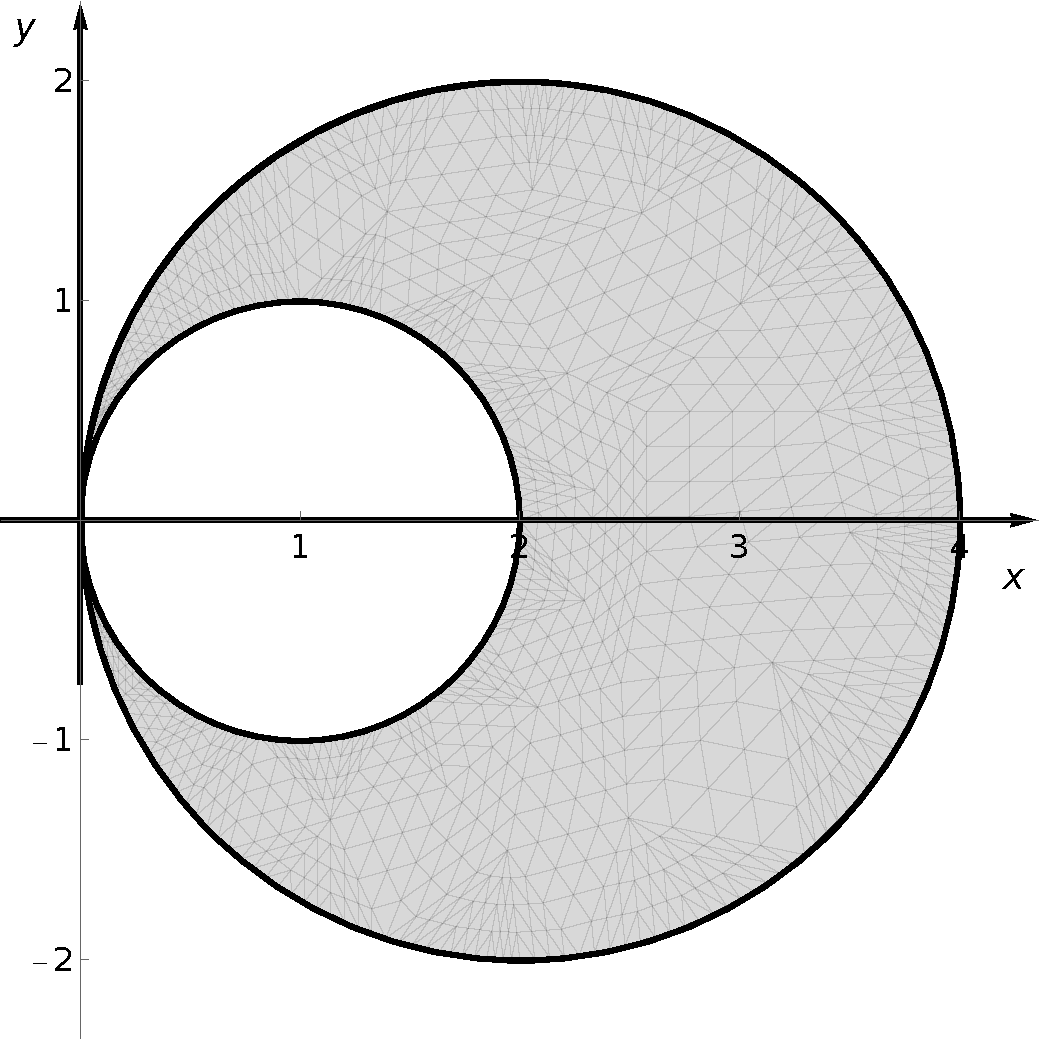
\includegraphics[width=0.43\textwidth]{fig_double_14a}}
\qquad
\subfigure[\label{fig_double_14b}]{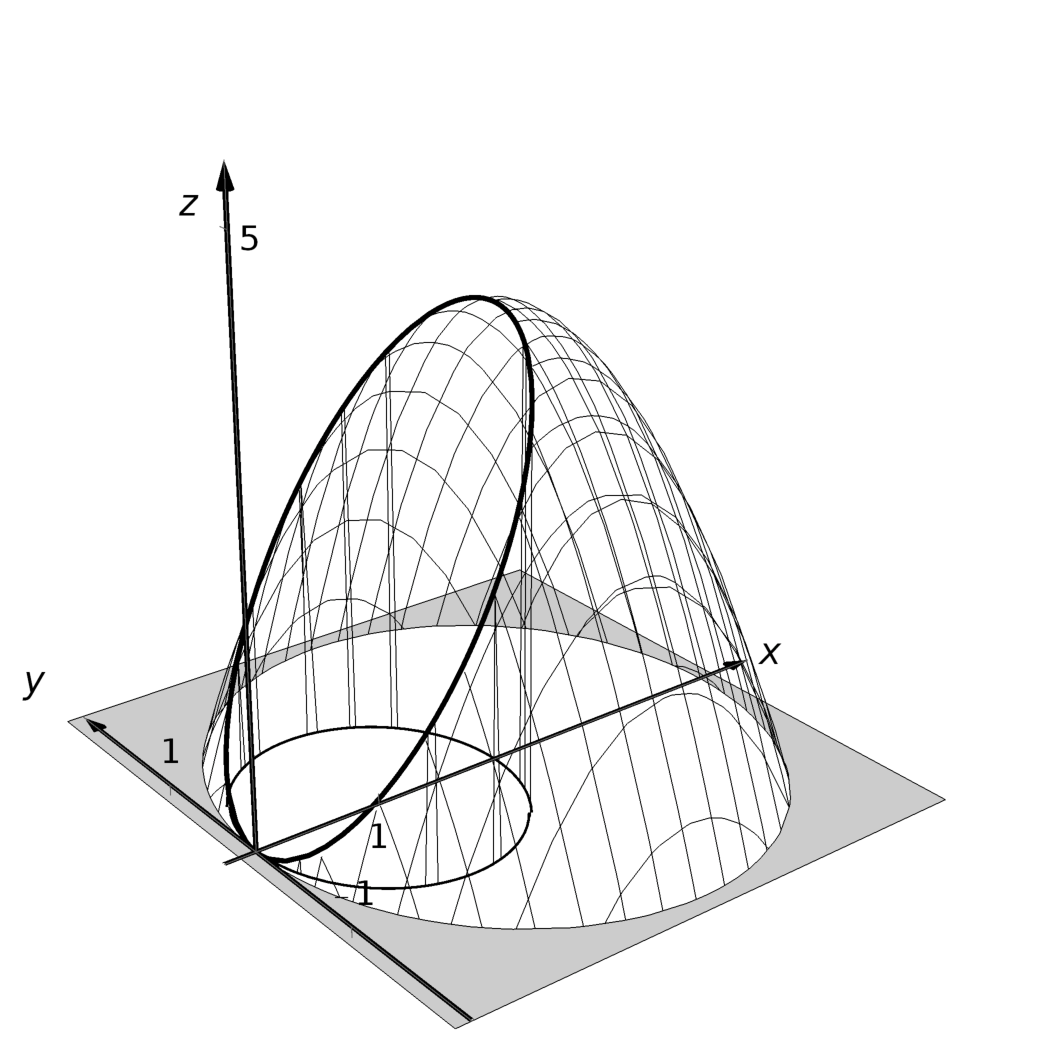
\includegraphics[width=0.43\textwidth]{fig_double_14b} }
\caption{Showing the region $R$ (a) and surface (b) used in Example \ref{ex_doublepol2}}
\end{figure}

\end{example}


%\ifanalysis
%\begin{example}\label{ex_doublepol5}
%
%Find the volume under the surface $\ds f(x,y) =\left(x^2+y^2+1\right)^{-1}$ over the  sector of the circle with radius $a$ centered at the origin in the first quadrant, as shown in Figure \ref{fig_double_15}.

%\begin{figure}[H]
%	\begin{center}
%			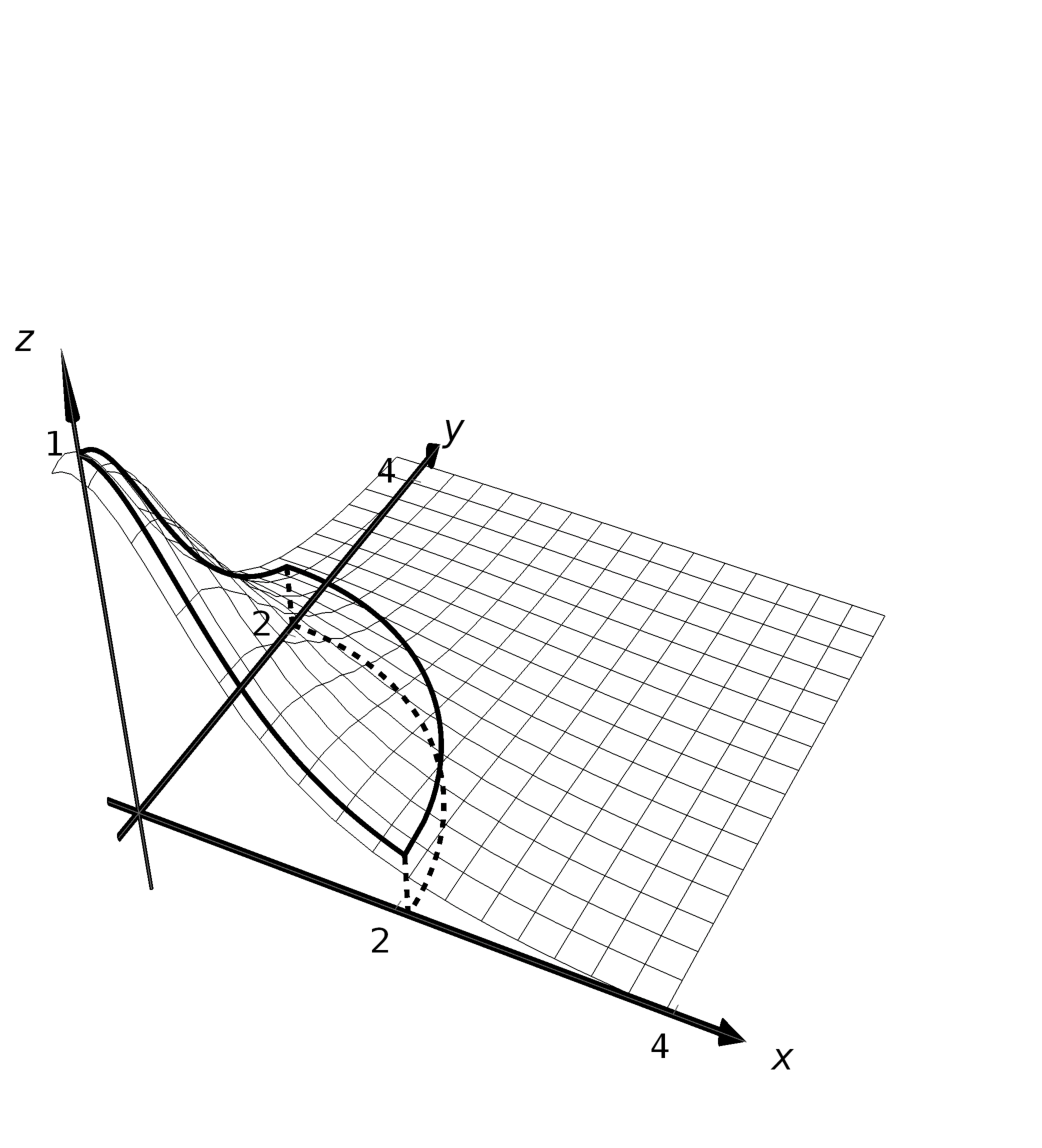
\includegraphics[width=0.5\textwidth]{fig_double_15}
%	\caption{The surface and region $R$ used in Example \ref{ex_doublepol5}.}
%	\label{fig_double_15}
%	\end{center}
%\end{figure}

%\xhrulefill{gray}{2.5pt}Solution \xhrulefill{gray}{2.5pt}

%The region $R$ we are integrating over is a circle with radius $a$, restricted to the first quadrant. Thus, in polar, the bounds on $R$ are $0\leq r\leq a$, $0\leq\theta\leq\pi/2$. The integrand is rewritten in polar coordinates as 
%$$\frac{1}{x^2+y^2+1} \quad  \Rightarrow \quad  \frac{1}{r^2\cos^2(\theta)+r^2\sin^2(\theta)+1} = \frac1{r^2+1}.$$
%We find the volume as follows:
%\begin{align*}
%\iint_Rf(x,y)\ dA &= \int\limits_0^{\pi/2}\int\limits_0^a\frac{r}{r^2+1}\ dr\ d\theta\\
%		&= \int\limits_0^{\pi/2} \frac12\big(\ln|r^2+1|\big)\Big|_0^a\ d\theta\\
%		&=\int\limits_0^{\pi/2} \frac12\ln(a^2+1)\ d\theta\\
%		&= \left.\left(\frac12\ln(a^2+1)\theta\right)\right|_0^{\pi/2}\\
%		&= \frac{\pi}{4}\ln(a^2+1).
%\end{align*}
%Figure \ref{fig_double_15}  shows that $f$ shrinks to near 0 very quickly. Regardless, as $a$ grows, so does the volume, without bound.
% 
%\end{example}
%\fi

\begin{example}\label{ex_doublepol3}
Find the volume of a sphere with radius $a$.

\xhrulefill{gray}{2.5pt}Solution \xhrulefill{gray}{2.5pt}


The sphere of radius $a$, centred at the origin, has equation $x^2+y^2+z^2=a^2$; solving for $z$, we have $$z=\pm\sqrt{a^2-x^2-y^2}.$$ The half solution $z>0$  gives the upper half of a sphere. We wish to find the volume under this top half, then double it to find the total volume. 

The region we need to integrate over is the disk of radius $a$, centred at the origin. Polar bounds for this equation are $0\leq r\leq a$, $0\leq\theta\leq2\pi$.

All together, the volume of a sphere with radius $a$ is:
\allowdisplaybreaks
\begin{align*}
2\iint_R\sqrt{a^2-x^2-y^2}\ dA &= 2\int\limits_0^{2\pi}\int\limits_0^a\sqrt{a^2-\Big(r\cos(\theta)\Big)^2-\Big(r\sin(\theta)\Big)^2}r\ dr\ d\theta\\
		&=2\int\limits_0^{2\pi}\int\limits_0^ar\sqrt{a^2-r^2}\ dr\ d\theta.
\intertext{We can evaluate this inner integral with substitution. With $u=a^2-r^2$, $du = -2r\ dr$. The new bounds of integration are $u(0) = a^2$ to $u(a)=0$. Thus we have:}
	&= \int\limits_0^{2\pi}\int\limits_{a^2}^0\big(-u^{1/2}\big)\ du\ d\theta\\
	&= \int\limits_0^{2\pi}\left.\left(-\frac23u^{3/2}\right)\right|_{a^2}^0 d\theta\\
	&= \int\limits_0^{2\pi}\left(\frac23a^3\right)\ d\theta\\
	&= \left.\left(\frac23a^3\theta\right)\right|_0^{2\pi}\\
	&= \frac43\pi a^3.
\end{align*}
Generally, the formula for the volume of a sphere with radius $r$ is given as $4\pi r^3/3$; we have justified this formula with our calculation.
\end{example}

We have used iterated integrals to find areas of plane regions and volumes under surfaces. Just as a single integral can be used to compute much more than area under the curve, iterated integrals can be used to compute much more than we have thus far seen. The next two sections show two, among many, applications of iterated integrals.

\section{Centre of mass}\label{sec:center_of_mass}

We have used iterated integrals to find areas of plane regions and signed volumes under surfaces. Here, we will  apply iterated integrals to compute the \textbf{mass} and \textbf{centre of mass} (\textit{massamiddelpunt}) of planar regions.

\subsection{Mass and weight}
Consider a thin sheet of material with constant thickness and finite area. Mathematicians (and physicists and engineers) call such a sheet a lamina. So consider a lamina, as shown in Figure \ref{fig_double_15a},  with the shape of some planar region $R$, as shown in Figure~\ref{fig_double_15b}.

\begin{figure}
\centering
%\raisebox{0.5cm}{
\subfigure[\label{fig_double_15a}]{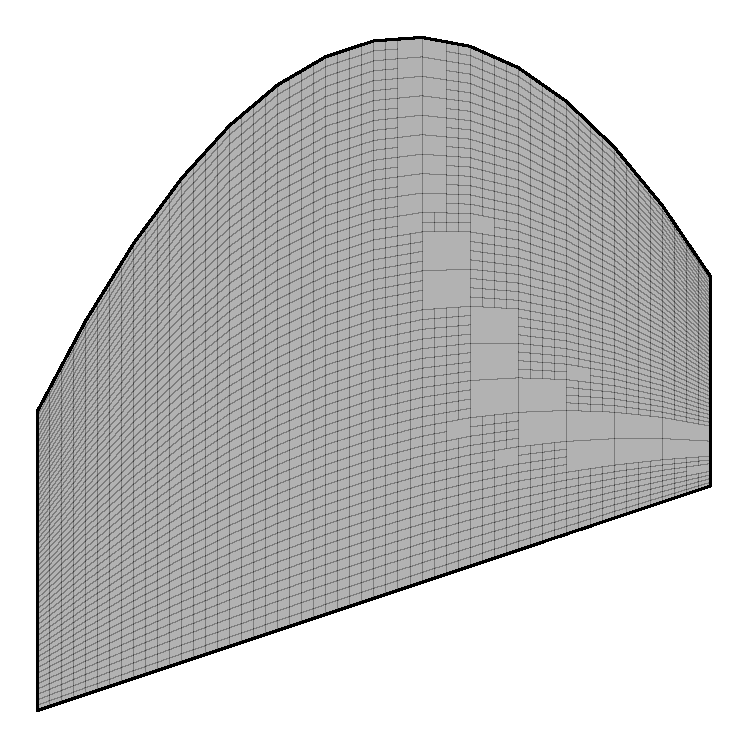
\includegraphics[width=0.43\textwidth]{fig_double_15a}}
\qquad
\subfigure[\label{fig_double_15b}]{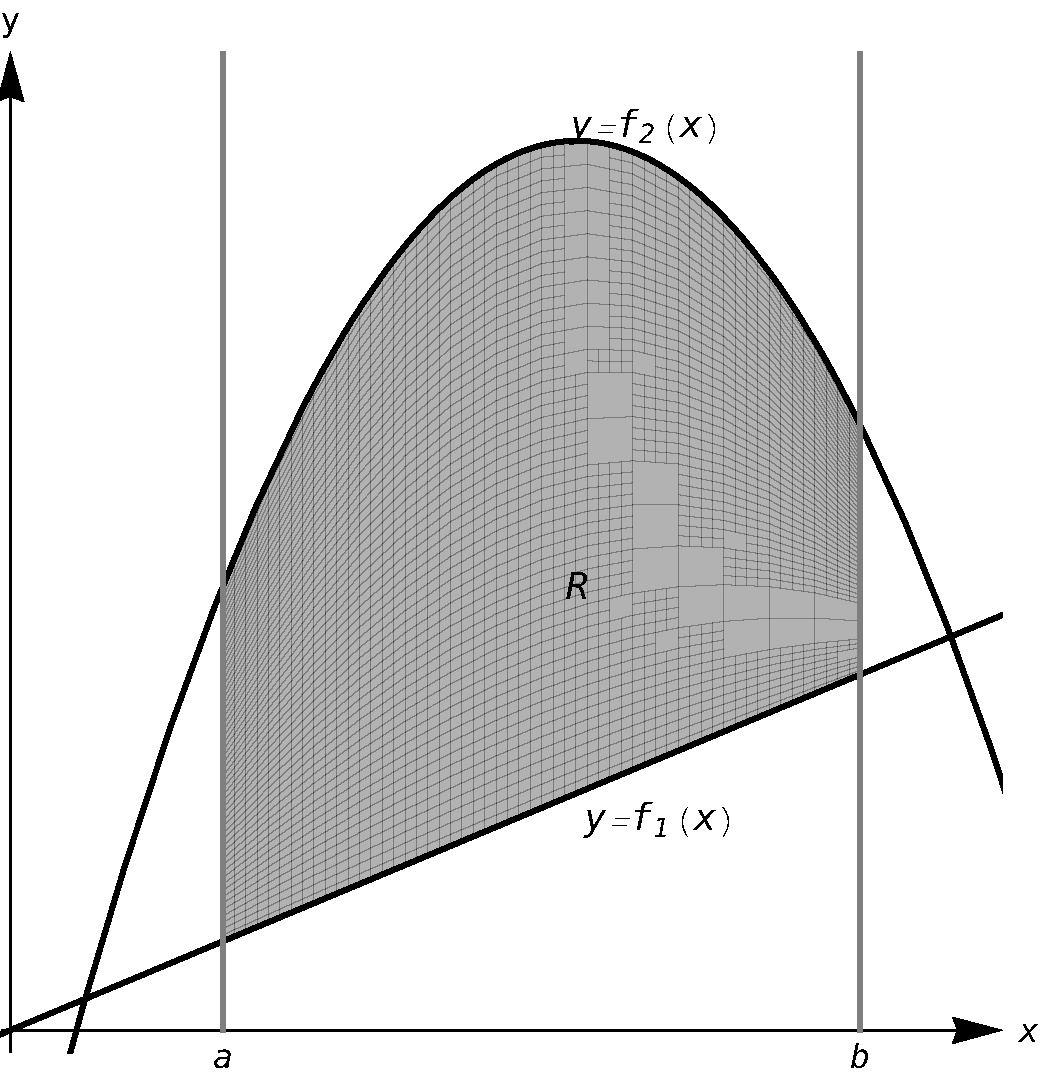
\includegraphics[width=0.43\textwidth]{fig_double_15b} }
\caption{Illustrating the concept of a lamina.}
\end{figure}


We can write a simple double integral that represents the mass of the lamina: $\iint_R\ dm$, where $dm$ means a little mass. That is, the double integral states the total mass of the lamina can be found by summing up lots of little masses over $R$. To evaluate this double integral, partition $R$ into $n$ subregions as we have done in the past. The $i^{\,\text{th}}$ subregion has area $\Delta A_i$. 
A fundamental property of mass is that ``mass=density$\times$area''. If the lamina has a constant density $\delta$, then the mass of this $i^{\,\text{th}}$ subregion is $\Delta m_i=\delta\Delta A_i$. %then $dm=\delta\ dA$. 
That is, we can compute a small amount of mass by multiplying a small amount of area by the density.

If density is variable, with density function $\delta= \delta(x,y)$, then we can approximate the mass of the $i^{\,\text{th}}$ subregion of $R$ by multiplying $\Delta A_i$ by $\delta(x_i,y_i)$, where $(x_i,y_i)$ is a point in that subregion. That is, for a small enough subregion of $R$, the density across that region is almost constant. 

Note that mass and weight are different measures. Since they are scalar multiples of each other, it is often easy to treat them as the same measure. Here,  we effectively treat them as the same, as our technique for finding mass is the same as for finding weight. The density functions used will simply have different units.

The total mass $M$ of the lamina is approximately the sum of approximate masses of subregions:
$$M \approx \sum_{i=1}^n \Delta m_i = \sum_{i=1}^n \delta(x_i,y_i)\Delta A_i.$$

Taking the limit as the size of the subregions shrinks to 0 gives us the actual mass; that is, integrating $\delta(x,y)$ over $R$ gives the mass of the lamina:
\begin{equation}
M = \iint_R\ dm = \iint_R \delta(x,y)\ dA.
\label{def:mass}
\end{equation}

\begin{example}\label{ex_mass2}
Find the mass of a square lamina, represented by the unit square with lower lefthand corner at the origin, with variable density $\delta(x,y) = (x+y+2)$g/cm$^2$.

\xhrulefill{gray}{2.5pt}Solution \xhrulefill{gray}{2.5pt}

The variable density $\delta$, in this example, is very uniform, giving a density of 3 in the centre of the square and changing linearly. A graph of $\delta(x,y)$ can be seen in Figure \ref{fig_double_16}; notice how same amount of density is above $z=3$ as below. We'll comment on the significance of this momentarily.

The mass $M$ is found by integrating $\delta(x,y)$ over $R$. The order of integration is not important; we choose $dx\ dy$ arbitrarily. Thus:
\allowdisplaybreaks
\begin{align*}
M = \iint_R(x+y+2)\ dA &= \int\limits_0^1\int\limits_0^1 (x+y+2)\ dx\ dy\\
		&= \int\limits_0^1\left.\left(\frac 12x^2+x(y+2)\right)\right|_0^1dy\\
		&= \int\limits_0^1 \left(\frac52+y\right)\ dy\\
		&= \left.\left(\frac52y+\frac12y^2\right)\right|_0^1=3\text{g}.
\end{align*}
It turns out that since the density of the lamina is so uniformly distributed above and below $z=3$ that the mass of the lamina is the same as if it had a constant density of 3. The density function $\delta=3$g/cm$^2$ and the one from this example are graphed in Figure \ref{fig_double_16}, which illustrates this concept.

\begin{figure}[H]
	\begin{center}
			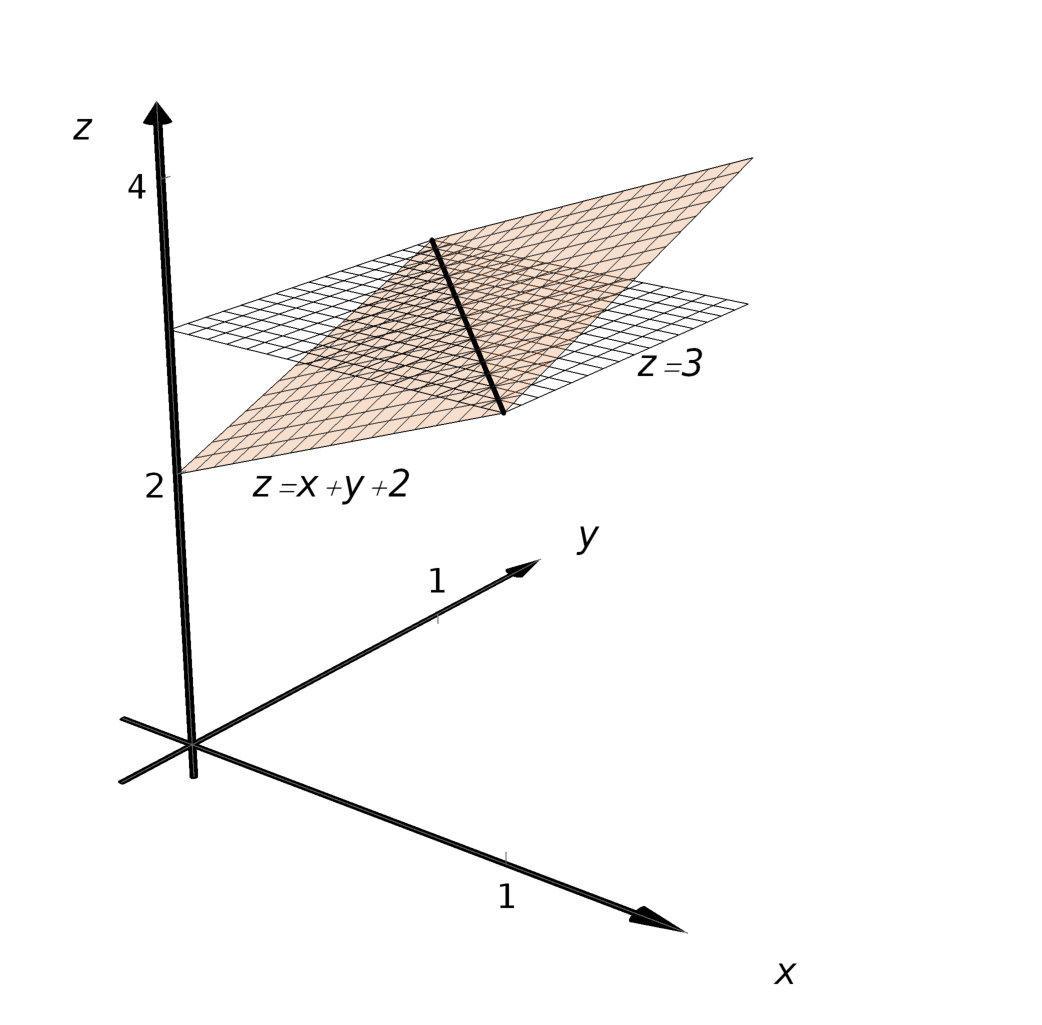
\includegraphics[width=0.5\textwidth]{fig_double_16}
	\caption{Graphing the density functions $\delta=3$g/cm$^2$ and $\delta(x,y) = (x+y+2)$g/cm$^2$.}
	\label{fig_double_16}
	\end{center}
\end{figure}


\end{example}

\begin{example}\label{ex_mass3}
Find the weight of the lamina represented by the disk with radius 2cm, centred at the origin, with density function $\delta(x,y) = (x^2+y^2+1)$g/cm$^2$. Compare this to the weight of the lamina with the same shape and density $\delta(x,y) = (2\sqrt{x^2+y^2}+1)$g/cm$^2$.

\xhrulefill{gray}{2.5pt}Solution \xhrulefill{gray}{2.5pt}

A direct application of Equation~\eqref{def:mass} states that the weight of the lamina is $\iint_R\delta(x,y)\ dA$. Since our lamina is in the shape of a circle, it makes sense to approach the double integral using polar coordinates.

The density function $\delta(x,y) = x^2+y^2+1$ becomes $$\delta(r,\theta) = (r\cos(\theta))^2+(r\sin(\theta))^2+1 = r^2+1.$$ The circle is bounded by $0\leq r\leq 2$ and $0\leq\theta\leq2\pi$. Thus the weight $W$ is:
\allowdisplaybreaks
\begin{align*}
W &= \int\limits_0^{2\pi}\int\limits_0^2 (r^2+1)r\ dr\ d\theta\\
	&= \int\limits_0^{2\pi} \left.\left(\frac14r^4+\frac12r^2\right)\right|_0^2d\theta\\
	&= \int\limits_0^{2\pi} 6 \ d\theta\\
	&= 12\pi \approx 37.70\text{g}.
\end{align*}

Now compare this with the density function $\delta(x,y) = 2\sqrt{x^2+y^2}+1$. Converting this to polar coordinates gives $$\delta(r,\theta) = 2\sqrt{\Big(r\cos(\theta)\Big)^2+\Big(r\sin(\theta)\Big)^2}+1 = 2r+1.$$ Thus the weight $W$ is:
\begin{align*}
W &= \int\limits_0^{2\pi}\int\limits_0^2 (2r+1)r\ dr\ d\theta\\
	&= \int\limits_0^{2\pi} \left(\frac23r^3+\frac12r^2\right)\Big|_0^2d\theta\\
	&= \int\limits_0^{2\pi} \left(\frac{22}3\right)\ d\theta\\
	&= \frac{44}3\pi \approx 46.08\text{g}.
\end{align*}
One would expect different density functions to return different weights, as we have here. The density functions were chosen, though, to be similar: each gives a density of 1 at the origin and a density of 5 at the outside edge of the circle, as seen in Figure \ref{fig_double_17}.


Notice how $x^2+y^2+1 \leq 2\sqrt{x^2+y^2}+1$ over the circle; this results in less weight.
\end{example}

\begin{figure}
\centering
%\raisebox{0.5cm}{
\subfigure[\label{fig_double_17a}]{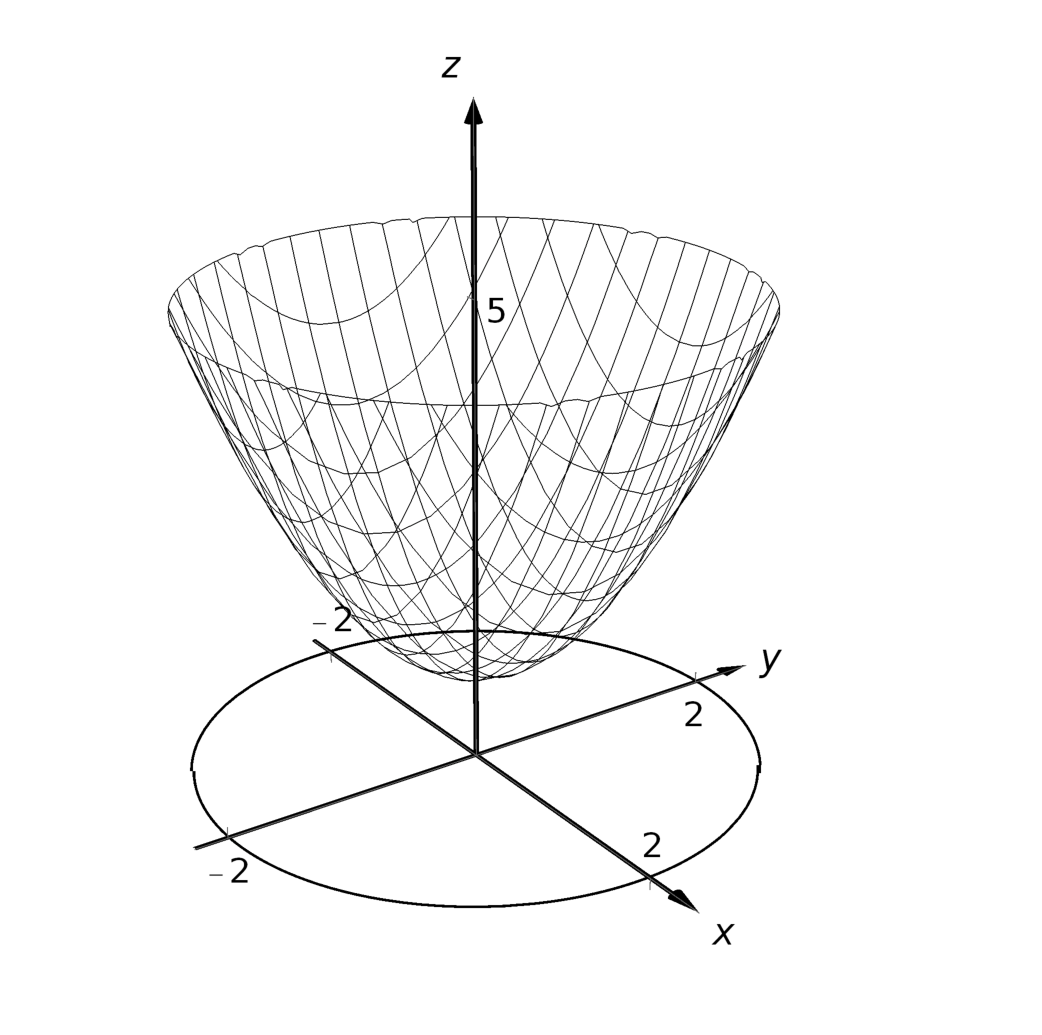
\includegraphics[width=0.43\textwidth]{fig_double_17a}}
\qquad
\subfigure[\label{fig_double_17b}]{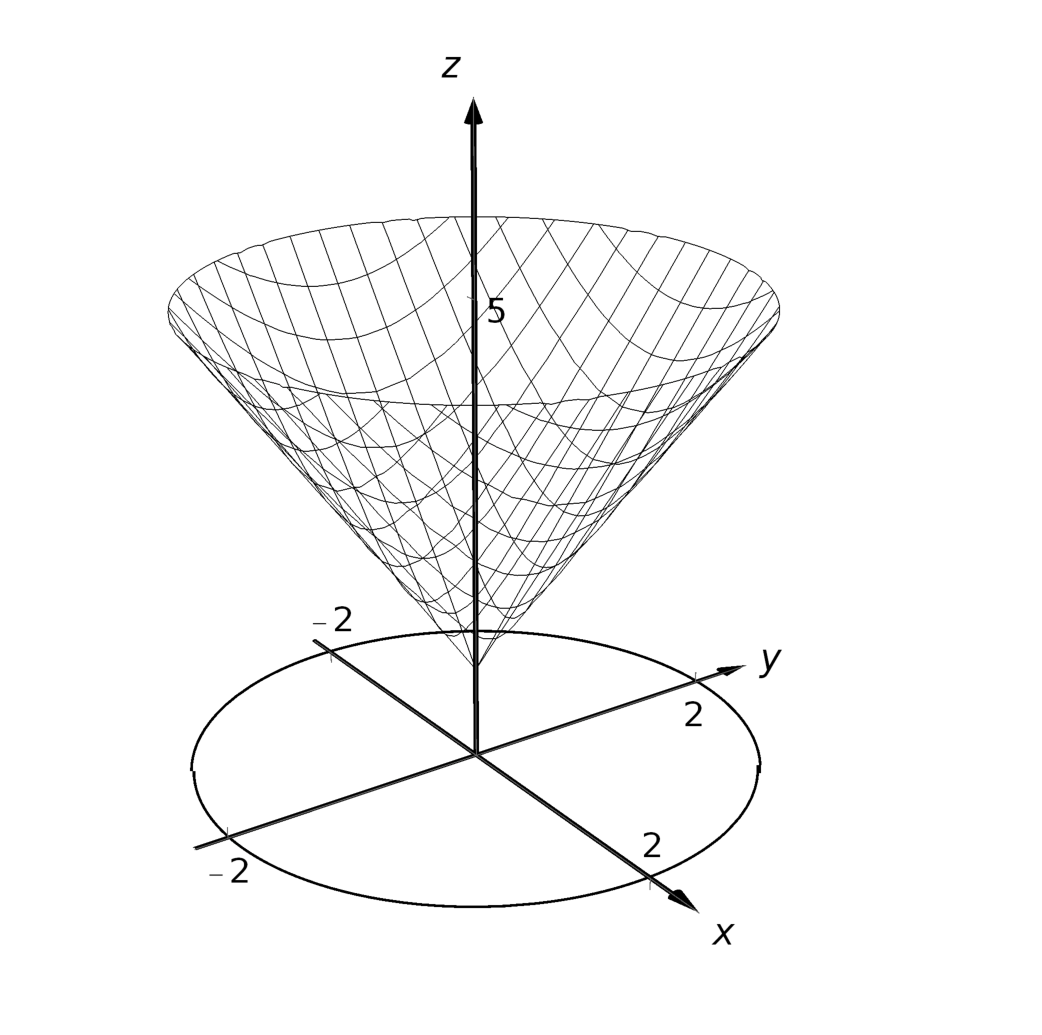
\includegraphics[width=0.43\textwidth]{fig_double_17b} }
\caption{Graphing the density functions  $\delta(x,y) = x^2+y^2+1$ (a) and $\delta(x,y) = 2\sqrt{x^2+y^2}+1$ (b).}
\label{fig_double_17}
\end{figure}

Plotting the density functions can be useful as our understanding of mass can be related to our understanding of volume under a surface. We interpreted $\iint_R f(x,y)\ dA$ as giving the volume under $f$ over $R$; we can understand $\iint_R\delta(x,y)\ dA$ in the same way. The volume under $\delta$ over $R$ is actually mass; by compressing the volume under $\delta$ onto the $xy$-plane, we get more mass in some areas than others -- i.e., areas of greater density.

Knowing the mass of a lamina is one of several important measures. Another is the centre of mass, which we discuss next.

\subsection{Centre of mass}

Consider a disk of radius 1 with uniform density. It is common knowledge that the disk will balance on a point if the point is placed at the centre of the disk. What if the disk does not have a uniform density? Through trial-and-error, we should still be able to find a spot on the disk at which the disk will balance on a point. This balance point is referred to as the \textbf{centre of mass} (\textit{massamiddelpunt}), or \textbf{centre of gravity} (\textit{zwaartepunt}). It is though all the mass is centred there. In fact, if the disk has a mass of 3kg, the disk will behave physically as though it were a point mass of 3kg located at its centre of mass. For instance, the disk will naturally spin with an axis through its centre of mass.
\index{centre of mass}\index[aut]{massamiddelpunt}

We find the centre of mass based on the principle of a weighted average. Consider a college class in which your homework average is 90\%, your test average is 73\%, and your final exam grade is an 85\%. Experience tells us that our final grade is not the \textit{average} of these three grades: that is, it is not:
$$\frac{0.9+0.73+0.85}{3} \approx 0.837 = 83.7\text{\%}.$$
That is, you are probably not pulling a B in the course. Rather, your grades are weighted. Let us say the homework is worth 10\% of the grade, tests are 60\% and the exam is 30\%. Then your final grade is:
$$(0.1)(0.9) + (0.6)(0.73)+(0.3)(0.85) = 0.783 = 78.3\text{\%}.$$
Each grade is multiplied by a weight. 

In general, given values $x_1,x_2,\ldots,x_n$ and weights $w_1,w_2,\ldots,w_n$, the weighted average of the $n$-values is
$$\dfrac{\ds\sum_{i=1}^n w_ix_i}{\ds\sum_{i=1}^n w_i}.$$

How this relates to centre of mass is given in the following definition.

\begin{definition}[Centre of mass of a discrete linear system]\label{thm:center_mass_points}
Let point masses $m_1,m_2,\ldots,m_n$ be distributed along the $x$-axis at locations $x_1,x_2,\ldots,x_n$, respectively. The \textbf{centre of mass $\overline{x}$} of the system is located at
\index{centre of mass}\index[aut]{massamiddelpunt}
$$\overline{x} = \dfrac{\ds\sum_{i=1}^nm_ix_i}{\ds\sum_{i=1}^n m_i}.$$
\end{definition}

In a discrete system (i.e., mass is located at individual points, not along a continuum) we find the centre of mass by dividing the mass into a \textbf{moment} (\textit{moment}) of the system. In general, a moment is a weighted measure of distance from a particular point or line. In the case described by Definition \ref{thm:center_mass_points}, we are finding a weighted measure of distances from the $y$-axis, so we refer to this as \textbf{the moment about the $y$-axis} (\textit{moment om de $y$-as}), represented by $M_y$.  Letting $M$ be the total mass of the system, we have  $\overline{x} = M_y/M$. 

We can extend the concept of the centre of mass of discrete points along a line to the centre of mass of discrete points in the plane rather easily. To do so, we define some terms then give a theorem.


\begin{definition}[Moments about the $x$- and $y$- axes]\label{def:moment}
Let point masses $m_1$, $m_2,\ldots,m_n$ be located at points $(x_1,y_1)$, $(x_2,y_2)\ldots,(x_n,y_n)$, respectively, in the $xy$-plane. \index{moment}\index[aut]{moment}
\begin{enumerate}
	\item The \textbf{moment about the $x$-axis}, $M_x$, is 
	$$\ds M_x = \sum_{i=1}^n m_iy_i.$$
	\item The \textbf{moment about the $y$-axis}, $M_y$, is 
	$$\ds M_y = \sum_{i=1}^n m_ix_i.$$
	\end{enumerate}
\end{definition}

We now define the centre of mass of discrete points in the plane.

\begin{definition}[Centre of mass of a discrete planar system]\label{thm:center_mass_points_plane}
Let point masses $m_1$, $m_2,\ldots,m_n$ be located at points $(x_1,y_1)$, $(x_2,y_2)\ldots,(x_n,y_n)$, respectively, in the $xy$-plane, and let $\ds M = \sum_{i=1}^n m_i$.  
\index{centre of mass}\index[aut]{massamiddelpunt}

The \textbf{centre of mass} of the system is at $(\overline{x},\overline{y})$, where 
$$\overline{x}= \frac{M_y}{M}\quad \text{and}\quad \overline{y} = \frac{M_x}{M}.$$

\end{definition}

\begin{example}\label{ex_mass5}
Let point masses of 1kg, 2kg and 5kg be located at points $(2,0)$, $(1,1)$ and $(3,1)$, respectively, and are connected by thin rods of negligible weight. Find the centre of mass of the system.

\pagebreak
\xhrulefill{gray}{2.5pt}Solution \xhrulefill{gray}{2.5pt}


We follow Definitions~\ref{thm:center_mass_points_plane} and \ref{def:moment} to find $M$, $M_x$ and $M_y$:

$M = 1+2+5 = 8$kg.

\noindent\begin{minipage}{.5\linewidth}
\begin{align*}
M_x &=  \sum_{i=1}^n m_iy_i \\
		&= 1(0) + 2(1) + 5(1) \\
		&= 7.
\end{align*}
\end{minipage}
\begin{minipage}{.5\linewidth}
\begin{align*}
M_y &=  \sum_{i=1}^n m_ix_i \\
		&= 1(2) + 2(1) + 5(3) \\
		&= 19.
\end{align*}
\end{minipage}

Thus the centre of mass is $$\ds (\overline{x},\overline{y}) = \left(\frac{M_y}{M},\frac{M_x}M\right) = \left(\frac{{19}}8,\frac78\right)  =(2.375,0.875),$$ illustrated in Figure \ref{fig_double_18}.

\begin{figure}[H]
	\begin{center}
			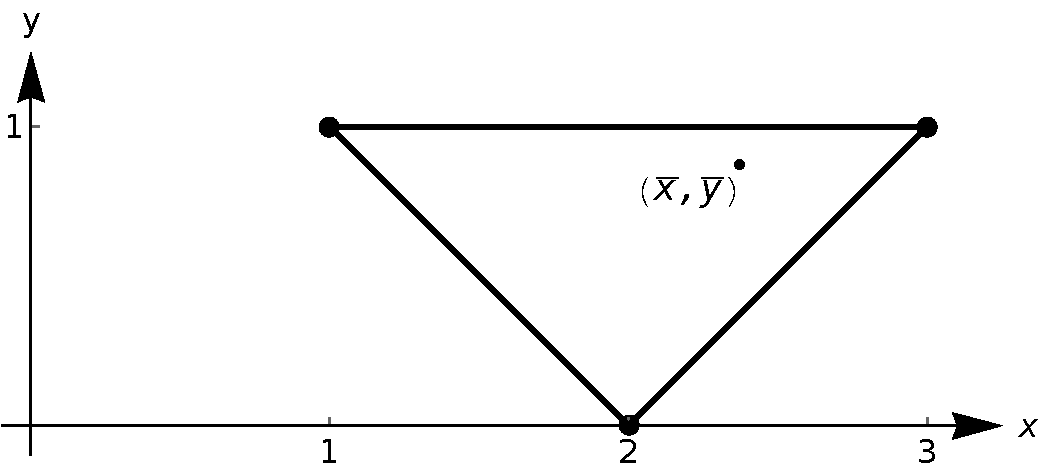
\includegraphics[width=0.5\textwidth]{fig_double_18}
	\caption{Illustrating the centre of mass of a discrete planar system in Example \ref{ex_mass5}.}
	\label{fig_double_18}
	\end{center}
\end{figure}

\end{example}

We finally arrive at our true goal of this section: finding the centre of mass of a lamina with variable density. While the above measurement of centre of mass is interesting, it does not directly answer more realistic situations where we need to find the centre of mass of a contiguous region. However, understanding the discrete case allows us to approximate the centre of mass of a planar lamina; using calculus, we can refine the approximation to an exact value.

We begin by representing a planar lamina with a region $R$ in the $xy$-plane with density function $\delta(x,y)$. Partition $R$ into $n$ subdivisions, each with area $\Delta A_i$. As done before, we can approximate the mass of the $i^{\,\text{th}}$ subregion with $\delta(x_i,y_i)\Delta A_i$, where $(x_i,y_i)$ is a point inside the $i^{\,\text{th}}$ subregion. We can approximate the moment of this subregion about the $y$-axis with $x_i\delta(x_i,y_i)\Delta A_i$ -- that is, by multiplying the approximate mass of the region by its approximate distance from the $y$-axis. Similarly, we can approximate the moment about the $x$-axis with $y_i\delta(x_i,y_i)\Delta A_i$. By summing over all subregions, we have:
\begin{align*}
\text{mass: } M &\approx \sum_{i=1}^n \delta(x_i,y_i)\Delta A_i\,, \qquad \text{(as seen before)}\\
\text{moment about the $x$-axis: } M_x &\approx \sum_{i=1}^n y_i\delta(x_i,y_i)\Delta A_i\,,\\
\text{moment about the $y$-axis: } M_y &\approx \sum_{i=1}^n x_i\delta(x_i,y_i)\Delta A_i\,.\\
\end{align*}

By taking limits, where size of each subregion shrinks to 0 in both the $x$- and $y$- directions, we arrive at the double integrals given in the following definition.

\begin{definition}[Centre of mass of a planar lamina]\label{thm:center_of_mass}
Let a planar lamina be represented by a closed, bounded region $R$ in the $xy$-plane with density function $\delta(x,y)$. Then we can infer the following information about the lamina: \index{centre of mass}\index{moment}\index[aut]{massamiddelpunt}\index[aut]{moment}
\begin{enumerate}
	\item The \textbf{mass} (\textit{massa}) of a planar lamina is $\ds M = \iint_R\delta(x,y)\ dA$.
	\item The \textbf{moment about the $x$-axis} is $\ds  M_x = \iint_Ry\delta(x,y)\ dA$.
	\item The \textbf{moment about the $y$-axis} is $\ds  M_y = \iint_Rx\delta(x,y)\ dA$.
	\item The \textbf{centre of mass} (\textit{massamiddelpunt}) of the object is
	$$(\overline{x},\overline{y}) = \left(\frac{M_y}{M},\frac{M_x}M\right).$$
\end{enumerate}
\end{definition}

We  practice  finding centres of mass by revisiting some of the lamina used previously in this section when finding mass. We will  just set up the integrals needed to compute $M$, $M_x$ and $M_y$ and leave the details of the integration to the reader.

\begin{example}
Find the centre of mass of a square lamina, represented by the unit square with lower lefthand corner at the origin (see Figure \ref{fig_double_16}), with variable density $\delta(x,y) = (x+y+2)$g/cm$^2$. This is the lamina from Example \ref{ex_mass2}.

\xhrulefill{gray}{2.5pt}Solution \xhrulefill{gray}{2.5pt}

We follow Theorem \ref{thm:center_of_mass}, to find $M$, $M_x$ and $M_y$:
\begin{align*}
M &= \iint_R (x+y+2)\ dA = \int\limits_0^1\int\limits_0^1 (x+y+2)\ dx\ dy =3\text{g}.\\
M_x &= \iint_R y(x+y+2)\ dA = \int\limits_0^1\int\limits_0^1 y(x+y+2)\ dx\ dy =\frac{19}{12}.\\
M_y &= \iint_R x(x+y+2)\ dA = \int\limits_0^1\int\limits_0^1 x(x+y+2)\ dx\ dy =\frac{19}{12}.
\end{align*}
Thus the centre of mass is $$\ds (\overline{x},\overline{y}) = \left(\frac{M_y}M,\frac{M_x}M\right) = \left(\frac{19}{36},\frac{19}{36}\right) \approx (0.528,0.528).$$ While the mass of this lamina is the same as the lamina in the previous example, the greater density found with greater $x$- and $y$-values pulls the centre of mass from the centre slightly towards the upper righthand corner.
\end{example}

\begin{example}\label{ex_mass8}
Find the centre of mass of the lamina represented by the circle with radius 2cm, centred at the origin, with density function $\delta(x,y) = (x^2+y^2+1)$g/cm$^2$. This is one of the lamina used in Example \ref{ex_mass3}.

\xhrulefill{gray}{2.5pt}Solution \xhrulefill{gray}{2.5pt}

As done in Example \ref{ex_mass3}, it is best to describe $R$ using polar coordinates.
Thus when we compute $M_y$, we will integrate not $x\delta(x,y) = x(x^2+y^2+1)$, but rather $\big(r\cos(\theta)\big)\delta(r\cos(\theta),r\sin(\theta))$\linebreak $= \big(r\cos(\theta)\big)\big(r^2+1\big).$ We compute $M$, $M_x$ and $M_y$:
\allowdisplaybreaks
\begin{align*}
M &= \int\limits_0^{2\pi}\int\limits_0^2 (r^2+1)r\ dr\ d\theta = 12\pi\approx 37.7\text{g}\,,\\
M_x &= \int\limits_0^{2\pi}\int\limits_0^2 (r\sin(\theta))(r^2+1)r \ dr\ d\theta = 0\,,\\
M_y &= \int\limits_0^{2\pi}\int\limits_0^2 (r\cos(\theta))(r^2+1)r \ dr\ d\theta = 0\,.\\
\end{align*}
Since $R$ and the density of $R$ are both symmetric about the $x$- and $y$-axes, it should come as no big surprise that the moments about each axis is 0. Thus the centre of mass is $(\overline{x},\overline{y})=(0,0)$. 
\end{example}

\section{Surface area}\label{sec:surface_area}
	\checkoddpage
\marginpar{\ifoddpage\hspace*{-1.5cm}\else\hspace*{0.25cm}\fi
\includegraphics[width=0.075\textwidth]{youtube}\\
\ifoddpage\hspace*{-1.75cm}\else\hspace*{0.1cm}\fi
\qrcode[height=1.75cm]{https://youtu.be/GSDrQYq_Iww}
%\includegraphics[width=0.1\textwidth]{surface_area_double}
}

In Section \ref{sec:arc_length} we used definite integrals to compute the arc length of plane curves of the form \linebreak $y=f(x)$. We later extended these ideas to compute the arc length of plane curves defined by parametric or polar equations. 

The natural extension of the concept of arc length over an interval to surfaces is surface area over a region. For that purpose, consider the surface $z=f(x,y)$ over a region $R$ in the $xy$-plane, shown in Figure \ref{fig_double_19a}. Because of the domed shape of the surface, the surface area will be greater than that of the area of the region $R$. We can find this area using the same basic technique we have used over and over: we'll make an approximation, then using limits, we'll refine the approximation to the exact value.


\begin{figure}
\centering
%\raisebox{0.5cm}{
\subfigure[\label{fig_double_19a}]{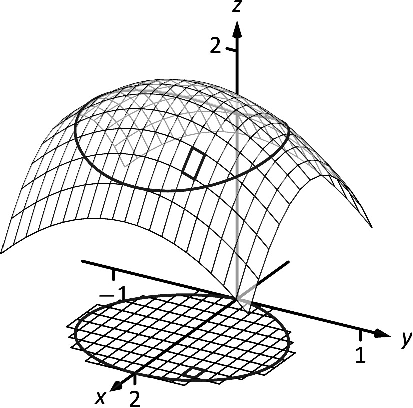
\includegraphics[width=0.43\textwidth]{fig_double_19a}}
\qquad
\subfigure[\label{fig_double_19b}]{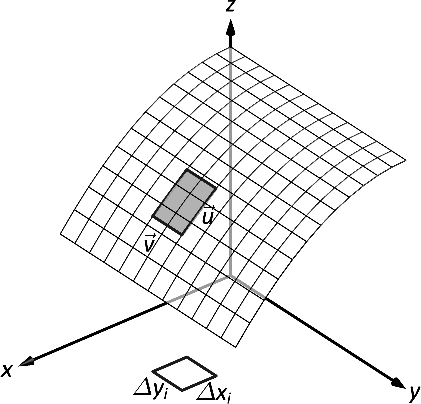
\includegraphics[width=0.43\textwidth]{fig_double_19b} }
\caption{Developing a method of computing surface area.}
\end{figure}



As done to find the volume under a surface or the mass of a lamina, we subdivide $R$ into $n$ subregions. Here we subdivide $R$ into rectangles, as shown in the figure. One such subregion is outlined in the figure, where the rectangle has dimensions $\dx_i$ and $\dy_i$, along with its corresponding region on the surface.

In Figure~\ref{fig_double_19b}, we zoom in on this portion of the surface. When $\dx_i$ and $\dy_i$ are small, the function is approximated well by the tangent plane at any point $(x_i,y_i)$ in this subregion, which is graphed in part (b). In fact, the tangent plane approximates the function so well that in this figure, it is virtually indistinguishable from the surface itself! Therefore we can approximate the surface area $S_i$ of this region of the surface with the area $T_i$ of the corresponding portion of the tangent plane.

This portion of the tangent plane is a parallelogram, defined by sides $\vec u$ and $\vec v$, as shown. One of the applications of the cross product from Section \ref{sec:cross_product} is that the area of this parallelogram is $\norm{\vec u\times \vec v}$. So, once we can determine $\vec u$ and $\vec v$, we can determine the area.

$\vec u$ is tangent to the surface in the direction of $x$, therefore, from Section \ref{sec:multi_tangent}, $\vec u$ is parallel to $\left( 1,0,f_x(x_i,y_i)\right)$. The $x$-displacement of $\vec u$ is $\dx_i$, so we know that $\vec u = \dx_i\left( 1,0,f_x(x_i,y_i)\right)$. Similar logic shows that $\vec v = \dy_i\left( 0,1,f_y(x_i,y_i)\right)$.Thus:
\begin{align*}
\text{surface area $S_i$} &\approx \text{area of  $T_i$}\\
				&= \norm{\vec u\times \vec v}\\[0.2cm]
				&= \big|\big|\dx_i\left( 1,0,f_x(x_i,y_i)\right)\times\dy_i\left( 0,1,f_y(x_i,y_i)\right)\big|\big|\\[0.2cm]
				&=\sqrt{1+f_x(x_i,y_i)^2+f_y(x_i,y_i)^2}\dx_i\dy_i.
\end{align*}
Note that $\dx_i\dy_i = \Delta A_i$, the area of the $i^{\,\text{th}}$ subregion.

Summing up all $n$ of the approximations to the surface area gives
$$\text{surface area over $R$} \approx \sum_{i=1}^n \sqrt{1+f_x(x_i,y_i)^2+f_y(x_i,y_i)^2}\Delta A_i.$$

Once again take a limit as all of the $\dx_i$ and $\dy_i$ shrink to 0; this leads to a double integral:
\begin{equation}
SA=\iint_R \sqrt{1+f_x(x,y)^2+f_y(x,y)^2}\ dA.
\label{def:surfacearea}
\end{equation}

We use this definition to compute surface areas of known surfaces. 

\begin{example}\label{ex_surfacearea2}
Find the surface area of the sphere with radius $a$ centred at the origin, whose top hemisphere has equation $f(x,y)=\sqrt{a^2-x^2-y^2}$. 

\pagebreak
\xhrulefill{gray}{2.5pt}Solution \xhrulefill{gray}{2.5pt}

We start by computing partial derivatives and find 
$$f_x(x,y) = \frac{-x}{\sqrt{a^2-x^2-y^2}} \quad \text{and}\quad f_y(x,y) = \frac{-y}{\sqrt{a^2-x^2-y^2}}.$$
As our function $f$ only defines the top upper hemisphere of the sphere, we double our surface area result to get the total area:
\begin{align*}
SA & = 2\iint_R \sqrt{1+ f_x(x,y)^2+f_y(x,y)^2}\ dA \\
		&= 2\iint_R \sqrt{1+ \frac{x^2+y^2}{a^2-x^2-y^2}}\ dA.
\end{align*}
The region $R$ that we are integrating over is bounded by the circle, centered at the origin, with radius $a$: $x^2+y^2=a^2$. Because of this region, we are likely to have greater success with our integration by converting to polar coordinates. Using the substitutions $x=r\cos(\theta)$, $y=r\sin(\theta)$, $dA = r\ dr\ d\theta$ and bounds $0\leq\theta\leq2\pi$ and $0\leq r\leq a$, we have:
\begin{align}
SA &= 2\int\limits_0^{2\pi}\int\limits_0^a \sqrt{1+\frac{r^2\cos^2(\theta)+r^2\sin^2(\theta)}{a^2-r^2\cos^2(\theta)-r^2\sin^2(\theta)}}\ r\ dr\ d\theta \notag\\
&=2\int\limits_0^{2\pi}\int\limits_0^ar\sqrt{1+\frac{r^2}{a^2-r^2}}\ dr\ d\theta\notag\\
&=2\int\limits_0^{2\pi}\int\limits_0^ar\sqrt{\frac{a^2}{a^2-r^2}}\ dr\ d\theta.\label{eq:exsurfacearea2}
\intertext{Apply substitution $u=a^2-r^2$ and integrate the inner integral, giving}
&= 2\int\limits_0^{2\pi} a^2\ d\theta\notag\\
&= 4\pi a^2\notag.
\end{align}
Our work confirms the known formula.

Note that the inner integral in Equation \eqref{eq:exsurfacearea2} is an improper integral, as its is not defined at $r=a$. To properly evaluate this integral, one must use the techniques of Section \ref{sec:improper_integration}.  Since the resulting improper integral does converge, the surface area is accurately computed.
\end{example}

\begin{example}\label{ex_surfacearea4}
Find the area of the surface $f(x,y) = x^2-3y+3$ over the region $R$ bounded by $-x\leq y\leq x$, $0\leq x\leq 4$, as pictured in Figure \ref{fig_double_20}.

\begin{figure}[H]
	\begin{center}
			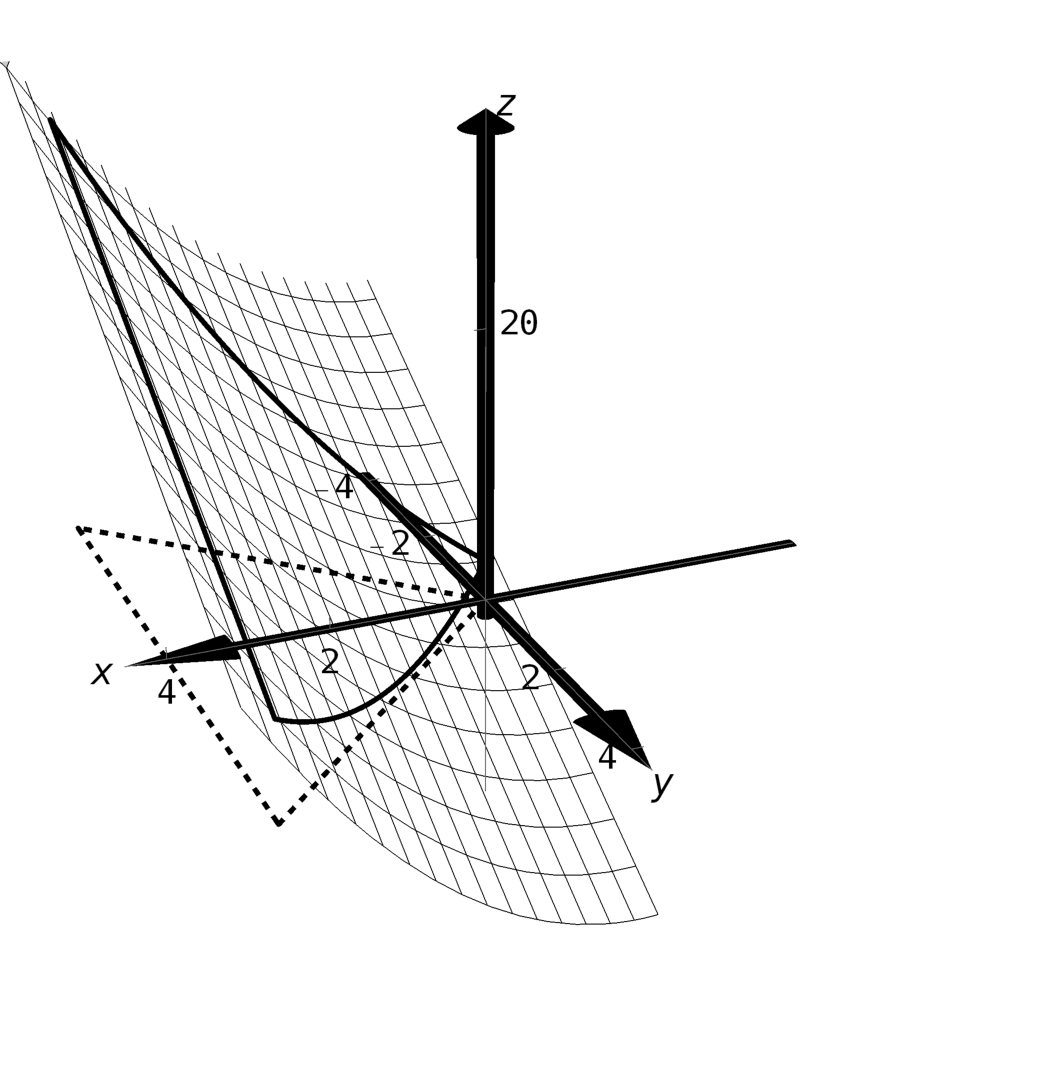
\includegraphics[width=0.5\textwidth]{fig_double_20}
	\caption{Graphing the surface in Example \ref{ex_surfacearea4}.}
	\label{fig_double_20}
	\end{center}
\end{figure}

\xhrulefill{gray}{2.5pt}Solution \xhrulefill{gray}{2.5pt}

It is straightforward to compute $f_x(x,y) = 2x$ and $f_y(x,y) = -3$. Thus the surface area is described by the double integral
$$\iint_R \sqrt{1+(2x)^2+(-3)^2}\ dA = \iint_R \sqrt{10+4x^2}\ dA.$$
As with integrals describing arc length, double integrals describing surface area are in general hard to evaluate directly because of the square root. This particular integral can be easily evaluated, though, with judicious choice of our order of integration. 

Integrating with order $dx\ dy$ requires us to evaluate $\int\limits \sqrt{10+4x^2}\ dx$. This can be done, though it involves the goniometric substitution $2x=\sqrt{10}\,\tan(t)$. Integrating with order $dy\ dx$ has as its first integral $\int\limits \sqrt{10+4x^2}\ dy$, which is easy to evaluate: it is simply $y\sqrt{10+4x^2}+C$. So we proceed with the order $dy\ dx$.
\allowdisplaybreaks
\begin{align*}
SA &= \iint_R\sqrt{10+4x^2}\ dA \\
            &= \int\limits_0^4\int\limits_{-x}^x\sqrt{10+4x^2}\ dy \ dx\\
				&= \int\limits_0^4\left.\left(y\sqrt{10+4x^2}\right)\right|_{-x}^x dx\\
				&=\int\limits_0^4 2x\sqrt{10+4x^2} \ dx
				\intertext{Apply substitution with $u = 10+4x^2$:}
			SA	&= \left.\left(\frac16\big(10+4x^2\big)^{3/2}\right)\right|_0^4 \\
				&= \frac13\big(37\sqrt{74}-5\sqrt{10}\big) \approx 100.825\text{ units}^2.
\end{align*}
So while the region $R$ over which we integrate has an area of 16 \text{units}$^2$, the surface has a much greater area as its $z$-values change dramatically over $R$.
\end{example}


In practice, technology helps greatly in the evaluation of such integrals. High powered computer algebra systems can compute integrals that are difficult, or at least time consuming, by hand, and can at least produce very accurate approximations with numerical methods. In general, just knowing how to set up the proper integrals brings one very close to being able to compute the needed value. Most of the work is actually done in just describing the region $R$ in terms of polar or rectangular coordinates. Once this is done, technology can usually provide a good answer.


\section{Line integrals over a scalar field}\label{sec:line_int_intro}
This section explores completely different relationships between vectors and integration. These relationships will enable us to compute the work done by a magnetic field in moving an object along a path and find how much air moves through an oddly--shaped screen in space, among other things. 

\subsection{Definition}
Consider the surface and curve shown in Figure \ref{fig_double_21a}. The surface is given by $$f(x,y)=1-\cos(x)\sin(y).$$
The dashed curve lies in the $xy$-plane and is the familiar $y=x^2$ parabola from $-1\leq x\leq1$; we will call this curve $C$. The curve drawn with a solid line in the graph is the curve in space that lies on our surface with $x$- and $y$- values that lie on $C$. 

The question we want to answer is this: what is the area that lies below the curve drawn with the solid line? In other words, what is the area of the region above $C$ and under the the surface $f$? This region is shown in Figure \ref{fig_double_21b}. We suspect the answer can be found using an integral, but before trying to figure out what that integral is, let us first try to approximate its value. 


\begin{figure}[t]
\centering
%\raisebox{0.5cm}{
\subfigure[\label{fig_double_21a}]{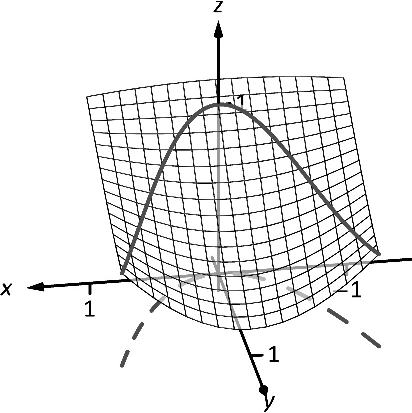
\includegraphics[width=0.33\textwidth]{fig_double_21a}}
\qquad
\subfigure[\label{fig_double_21b}]{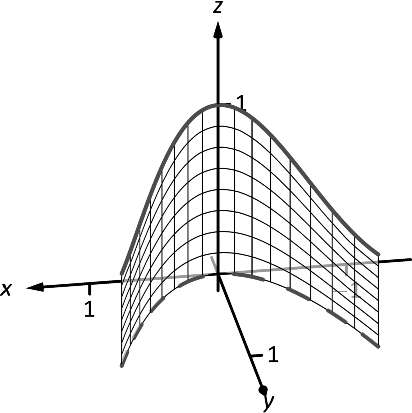
\includegraphics[width=0.33\textwidth]{fig_double_21b} }
\qquad
\subfigure[\label{fig_double_21c}]{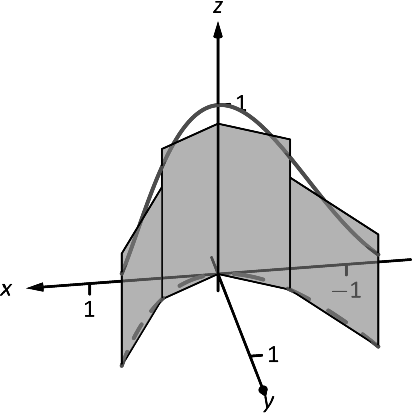
\includegraphics[width=0.33\textwidth]{fig_double_21c} }
\caption{Finding area under a curve in space.}
\end{figure}


In Figure \ref{fig_double_21c}, four rectangles have been drawn over the curve $C$. The bottom corners of each rectangle lie on $C$, and each rectangle has a height given by the function $f(x,y)$ for some $(x,y)$ pair along $C$ between the rectangle's bottom corners. 
As we know how to find the area of each rectangle, we are able to approximate the area above $C$ and under $f$. Clearly, our approximation will be an approximation. The heights of the rectangles do not match exactly with the surface $f$, nor does the base of each rectangle follow perfectly the path of $C$.

In typical calculus fashion, our approximation can be improved by using more rectangles. The sum of the areas of these rectangles gives an approximate value of the true area above $C$ and under $f$. As the area of each rectangle is height $\times$ width, we assert that the
$$\text{area above $C$}\approx \sum (\text{heights}\times\text{widths}).$$

When first learning of the integral, and approximating areas with (heights $\times$ widths), the width was a small change in $x$: $dx$. That will not suffice in this context. Rather, each width of a rectangle is actually approximating the arc length of a small portion of $C$. In Section \ref{sec:curvature}, we used $s$ to represent the arc length parameter of a curve. Hence, a small amount of arc length will thus be represented by $ds$. 

The height of each rectangle will be determined in some way by the surface $f$. If we parametrize $C$ by $s$, an $s$-value corresponds to an $(x,y)$ pair that lies on the parabola $C$. Since $f$ is a function of $x$ and $y$, and $x$ and $y$ are functions of $s$, we can say that $f$ is a function of $s$. Given a value $s$, we can compute $f(s)$ and find a height. Thus
\begin{align}
\text{area under $f$ and above $C$}&\approx \sum (\text{heights}\times\text{widths});\notag\\
		\text{area under $f$ and above $C$}							&=\lim_{\mathcal{L}\to0}\sum f(c_i)\Delta s_i\notag\\
									&=\int_Cf(s)\ ds.\label{eq:line0}
\end{align}

Here we have introduce a new notation, the integral symbol with a subscript of $C$. It is reminiscent of our usage of $\iint_R$. Using the train of thought found in the Integration Review preceding this section, we interpret $\int_C f(s)\ ds$ as meaning sum up, along a curve $C$, function values $f(s)$ $\times$ small arc lengths. It is understood here that $s$ represents the arc length parameter.

All this leads us to a definition. The integral found in Equation \ref{eq:line0} is called a \textbf{line integral}. We formally define it below.

\begin{definition}[Line integral over a scalar field]\label{def:line_integral1}
Let $C$ be a smooth curve parametrized by $s$, the arc length parameter, and let $f$ be a continuous function of $s$. A \textbf{line integral} (\textit{lijnintegraal}) is an integral of the form
$$\int_C f(s)\ ds = \lim_{\mathcal{L}\to 0}\sum_{i=1}^n f(c_i)\Delta s_i,$$
where $s_1<s_2<\cdots<s_n$ is any partition of the $s$-interval over which $C$ is defined, $c_i$ is any value in the $i\,^\text{th}$ subinterval,  $\Delta s_i$ is the width of the $i\,^\text{th}$ subinterval, and $\mathcal{L}$ is the length of the longest subinterval in the partition.\index{line integral}\index[aut]{lijnintegraal}%
\end{definition}

Note that Definition \ref{def:line_integral1} uses the term scalar field which has not yet been defined. Its meaning is discussed in  when it is compared to a vector field. Besides, when $C$ is a closed curve, i.e., a curve that ends at the same point at which it starts,  we use 
$$
\oint_C f(s)\ ds$$
instead of
$$
\quad \int_C f(s)\ ds.$$

The definition of the line integral does not specify whether $C$ is a curve in the plane or space (or hyperspace), as the definition holds regardless. For now, however, we will assume $C$ lies in the $xy$-plane.

Actually, this definition of the line integral  does not really say anything new. If $C$ is a curve and $s$ is the arc length parameter of $C$ on $a\leq s\leq b$, then 
$$\int_Cf(s)\ ds = \int\limits_a^bf(s)\ ds.$$
The real difference with this integral from the standard $\int\limits_a^bf(x)\ dx$ we used in the past is that of context. Our previous integrals naturally summed up values over an interval on the $x$-axis, whereas now we are summing up values over a curve. If we can parametrize the curve with the arc length parameter, we can evaluate the line integral just as before. Unfortunately, parametrizing a curve in terms of the arc length parameter is usually very difficult, so we must develop a method of evaluating line integrals using a different parametrization.

Given a curve $C$, find any parametrization of $C$: $x = g(t)$ and $y=h(t)$, for continuous functions $g$ and $h$, where $a\leq t\leq b$. We can represent this parametrization with a vector--valued function, \linebreak $\vrt = \left( g(t),h(t)\right)$.

In Section \ref{sec:curvature}, we defined the arc length parameter as 
$$
s(t) = \int\limits_0^t \norm{\vec r\,'(u)}\ du. 
$$
By the fundamental theorem of calculus, $ds = \norm{\vec r\,'(t)}\ dt$. We can substitute the right hand side of this equation for $ds$ in the line integral definition. Moreover, we can view $f$ as being a function of $x$ and $y$ since it is a function of $s$. Thus $f(s) =f(x,y) =f\big(g(t),h(t)\big)$. This gives us a concrete way to evaluate a line integral:
$$\int_C f(s)\ ds = \int\limits_a^bf\big(g(t),h(t)\big)\ \norm{\vec r\,'(t)}\ dt.$$

We restate this as a theorem for its $3$--dimensional analogue.


\begin{theorem}[Evaluating a line integral over a scalar field]\label{thm:line1}
Let $C$ be a curve parametrized by $\vrt =\left( g_1(t), g_2(t),g_3(t)\right)$, $a\leq t\leq b$, where $g_i$ is continuously differentiable, and let $z=f(\mathbf{x})$, where $f$ is continuous over $C$. Then\index{line integral!over scalar field}%
	$$\int_Cf(s)\ ds = \int\limits_a^bf\big(g_1(t),g_2(t),g_3(t)\big)\ \norm{\vec r\,'(t)}\ dt.$$
\end{theorem}


To be clear, the first point of Theorem \ref{thm:line1} can be used to find the area under a surface $z=f(x,y)$ and above a curve $C$. We will later give an understanding of the line integral when $C$ is a curve in space.

Let us do an example where we actually compute an area.

\begin{example}\label{ex_linescalarfield2}
Find the area under the surface $f(x,y) =\cos(x)+\sin(y)+2$ over the curve $C$, which is the segment of the line $y=2x+1$ on $-1\leq x\leq 1$, as shown in Figure \ref{fig_double_22}.

\begin{figure}[H]
\centering
%\raisebox{0.5cm}{
\subfigure[\label{fig_double_22a}]{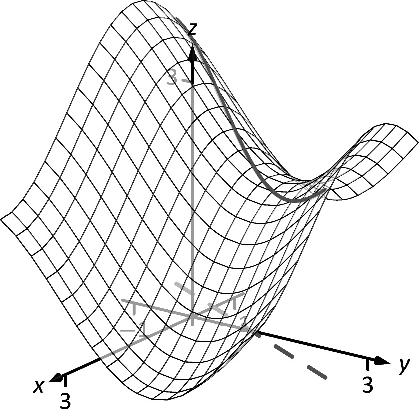
\includegraphics[width=0.43\textwidth]{fig_double_22a}}
\qquad
\subfigure[\label{fig_double_22b}]{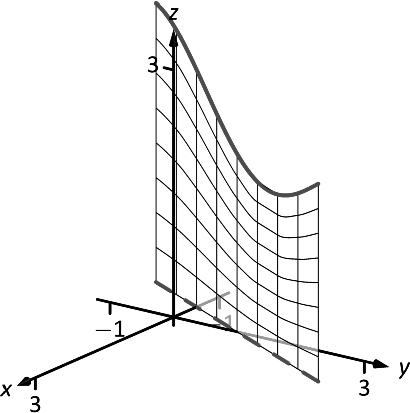
\includegraphics[width=0.43\textwidth]{fig_double_22b} }
\caption{Finding area under a curve in Example \ref{ex_linescalarfield2}.}
\label{fig_double_22}
\end{figure}

\pagebreak
\xhrulefill{gray}{2.5pt}Solution \xhrulefill{gray}{2.5pt}

Our first step is to represent $C$ with a vector--valued function. Since $C$ is a simple line, and we have a explicit relationship between $y$ and $x$ (namely, that $y=2x+1$), we can let $x = t$, $y = 2t+1$, and write $\vrt = \left( t, 2t+1\right)$ for $-1\leq t\leq 1$. 

We find the values of $f$ over $C$ as $$f(x,y) = f(t,2t+1) = \cos(t)+\sin(2t+1) + 2.$$ We also need \ $\norm{\vec r\,'(t)}$; with $\vrp(t) = \left(1,2\right)$, we have \ $\norm{\vrp(t)} = \sqrt{5}$. Thus $ds = \sqrt{5}\ dt$. 



The area we seek is 
\begin{align*}
\int_Cf(s)\ ds &= \int\limits_{-1}^1 \big(\cos(t)+\sin(2t+1) + 2\big)\sqrt{5}\ dt \\
					&= \left.\sqrt{5}\left(\sin(t) - \frac12\cos(2t+1)+2t\right)\right|_{-1}^1\\
					&\approx 14.418\ \text{units}^2.
\end{align*}



\end{example}

We now consider the example that introduced this section.\\

\begin{example}\label{ex_linescalarfield5}
Find the area under $f(x,y) = 1-\cos(x)\sin(y)$ and over the parabola $y = x^2$, from $-1\leq x\leq 1$. 

\xhrulefill{gray}{2.5pt}Solution \xhrulefill{gray}{2.5pt}

We parametrize our curve $C$ as $\vrt = \left( t,t^2\right)$ for $-1\leq t\leq 1$; we find $\norm{\vrp(t)} = \sqrt{1+4t^2}$, so $ds = \sqrt{1+4t^2}\ dt$. 

Replacing $x$ and $y$ with their respective functions of $t$, we have $$f(x,y) = f(t,t^2) = 1-\cos(t)\sin\left(t^2\right).$$ Thus the area under $f$ and over $C$ is found to be
$$
\int_C f(s)\ ds = \int\limits_{-1}^1 \Big(1-\cos(t)\sin\left(t^2\right)\Big)\sqrt{1+4t^2}\ dt.$$
This integral is impossible to evaluate using the techniques developed in this text. We resort to a numerical approximation; accurate to two places after the decimal, we find the area is 2.17.

\end{example}

Note how in each of the previous examples we are effectively finding area under a curve, just as we did when first learning of integration. We have used the phrase area over a curve $C$ and under a surface, but that is because of the important role $C$ plays in the integral. The figures show how the curve $C$ defines another curve on the surface $z=f(x,y)$, and we are finding the area under that curve.

\subsection{Properties}
Many properties of line integrals can be inferred from general integration properties. For instance, if $k$ is a scalar, then 
$$\int_C k\,f(s)ds = k\int_Cf(s)ds,$$
and similarly
$$\ds \int_C\big(f(s)+g(s)\big)\ ds = \int_Cf(s)\ ds +\int_Cg(s)\ ds,$$
where $f$ and $g$ are continuous functions of $s$.

One property in particular of line integrals is worth noting. If $C$ is a curve composed of subcurves $C_1$ and $C_2$, where they share only one point in common (see Figure \ref{fig_double_23a}), then the line integral over $C$ is the sum of the line integrals over $C_1$ and $C_2$: 
$$\int_Cf(s)\ ds = \int_{C_1}f(s)\ ds+\int_{C_2}f(s)\ ds.$$




This property allows us to evaluate line integrals over some curves $C$ that are not smooth. Note how in Figure \ref{fig_double_23b} the curve is not smooth at $D$, so by our definition of the line integral we cannot evaluate $\int_C f(s)ds$. However, one can evaluate line integrals over $C_1$ and $C_2$ and their sum will be the desired quantity. A curve $C$ that is composed of two or more smooth curves is said to be piecewise smooth. In this section, any statement that is made about smooth curves also holds for piecewise smooth curves.

\begin{figure}[H]
\centering
%\raisebox{0.5cm}{
\subfigure[\label{fig_double_23a}]{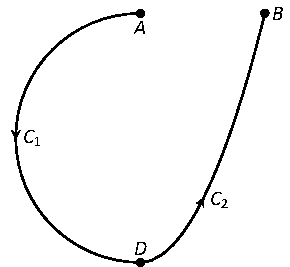
\includegraphics[width=0.25\textwidth]{fig_double_23a}}
\qquad
\subfigure[\label{fig_double_23b}]{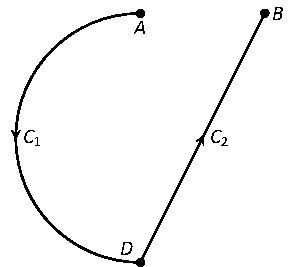
\includegraphics[width=0.25\textwidth]{fig_double_23b} }
\caption{Illustrating properties of line integrals.}
\end{figure}


\subsection{Centre of mass}
Let a curve $C$ (either in the plane or in space) represent a thin wire with variable density $\delta(s)$. We can approximate the mass of the wire by dividing the wire (i.e., the curve) into small segments of length $\Delta s_i$ and assume the density is constant across these small segments. The mass of each segment is density of the segment $\times$ its length; by summing up the approximate mass of each segment we can approximate the total mass:
$$\text{total mass of wire } \approx \sum\limits_i \delta(s_i)\Delta s_i.$$

By taking the limit as the length of the segments approaches 0, we have the definition of the line integral as seen in Definition \ref{def:line_integral1}. When learning of the line integral, we let $f(s)$ represent a height; now we let $f(s) = \delta(s)$ represent a density. We can extend this understanding of computing mass to also compute the centre of mass of a thin wire. We give the relevant formulas in the next definition, followed by an example.

\begin{definition}[Mass and centre of mass of a thin wire]\label{def:mass_of_thin_wire}
Let a thin wire lie along a smooth curve $C$ with continuous density function $\delta(s)$, where $s$ is the arc length parameter. 	\index{mass!centre of}\index[aut]{massamiddelpunt}\index{moment}\index[aut]{moment}%
\begin{enumerate}
	\item The \textbf{mass} (\textit{massa}) of the thin wire is $\ds M = \int_C \delta(s)\ ds$.
	\item The \textbf{moment about the $yz$-plane} is $\ds M_{yz} = \int_C x\delta(s)\ ds$.
	\item The \textbf{moment about the $xz$-plane} is $\ds M_{xz} = \int_C y\delta(s)\ ds$.
	\item The \textbf{moment about the $xy$-plane} is $\ds M_{xy} = \int_C z\delta(s)\ ds$.
	\item The \textbf{centre of mass} (\textit{massamiddelpunt}) of the wire is $$(\overline{x},\overline{y},\overline{z}) = \left(\frac{M_{yz}}M, \frac{M_{xz}}M,\frac{M_{xy}}M\right).$$
\end{enumerate}
\end{definition}


\begin{example}\label{ex_linescalarfield6}
A thin wire follows the path $\vrt = \left( 1+\cos(t),1+\sin(t), 1+ \sin(2t)\right)$, $0\leq t\leq 2\pi$. The density of the wire is determined by its position in space: $\delta(x,y,z) = y+z$ g/cm. The wire is shown in Figure \ref{fig_double_24}, where a light colour indicates low density and a dark colour represents high density. Find the mass  and centre of mass of the wire.


\begin{figure}[H]
	\begin{center}
			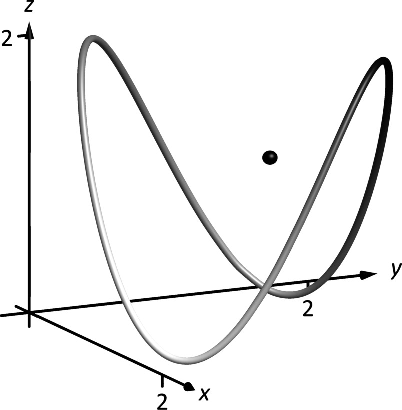
\includegraphics[width=0.38\textwidth]{fig_double_24}
	\caption{Finding the mass of a thin wire in Example \ref{ex_linescalarfield6}.}
	\label{fig_double_24}
	\end{center}
\end{figure}
\vspace*{-0.5cm}
\xhrulefill{gray}{2.5pt}Solution \xhrulefill{gray}{2.5pt}

We compute the density of the wire as 
$$\delta(x,y,z) = \delta\big(1+\cos(t),1+\sin(t), 1+\sin(2t)\big) = 2+\sin(t)+\sin(2t).$$ We compute $ds$ as
$$ds = \norm{\vrp(t)}\ dt = \sqrt{\sin^2(t)+\cos^2(t)+4\cos^2(2t)}\ dt = \sqrt{1+4\cos^2(2t)}\ dt.$$
Thus the mass is
$$M = \oint_C \delta(s)\ ds = \int\limits_0^{2\pi} \big(2+\sin(t)+\sin(2t)\big)\sqrt{1+4\cos^2(2t)}\ dt \approx 21.08 \text{ g }. $$
We compute the moments about the coordinate planes:%\small
\begin{align*}
M_{yz} &= \oint_C x\delta(s)\ ds = \int\limits_0^{2\pi}\big(1+\cos(t)\big)\big(2+\sin(t)+\sin(2t)\big)\sqrt{1+4\cos^2(2t)}\ dt \approx 21.08\, , \\
M_{xz} &= \oint_C y\delta(s)\ ds = \int\limits_0^{2\pi}\big(1+\sin(t)\big)\big(2+\sin(t)+\sin(2t)\big)\sqrt{1+4\cos^2(2t)}\ dt \approx
26.35\, ,\\
M_{xy} &= \oint_C z\delta(s)\ ds = \int\limits_0^{2\pi}\big(1+\sin(2 t)\big)\big(2+\sin(t)+\sin(2t)\big)\sqrt{1+4\cos^2(2t)}\ dt \approx 25.40.
\end{align*}%\normalsize
Thus the center of mass of the wire is located at 
$$(\overline{x},\overline{y},\overline{z}) = \left(\frac{M_{yz}}M, \frac{M_{xz}}M,\frac{M_{xy}}M\right) \approx (1,1.25,1.20),$$
as indicated by the dot in Figure \ref{fig_double_24}. Note how in this example, the curve $C$ is ''centered'' about the point $(1,1,1)$, though the variable density of the wire pulls the center of mass out along the $y$- and $z$-axes.
\end{example}


In the following, we investigate a new mathematical object, the vector field, after which we increase our understanding of integration in the context of vector fields.


\section{Vector fields}\label{sec:vector_fields}
\subsection{Definition}
	\checkoddpage
\marginpar{\ifoddpage\hspace*{-1.5cm}\else\hspace*{0.25cm}\fi
\includegraphics[width=0.075\textwidth]{youtube}\\
\ifoddpage\hspace*{-1.75cm}\else\hspace*{0.1cm}\fi
\qrcode[height=1.75cm]{https://youtu.be/gEa38ldV_a0}
%\includegraphics[width=0.1\textwidth]{fields}
}
We have studied functions, where the input of such functions is a point and the output is a number. We could also create functions where the input is a point, but the output is a  vector. For instance, we could create the following function: $\vec F(x,y) = \left( x+y, x-y\right)$, where $\vec F(2,3) = \left( 5,-1\right)$. We are to think of $\vec F$ assigning the vector $\left( 5,-1\right)$ to the point $(2,3)$; in some sense, the vector $\left( 5,-1\right)$ lies at the point $(2,3)$. 

Such functions are extremely useful in any context where magnitude and direction are important. For instance, we could create a function $\vec F$ that represents the electromagnetic force exerted at a point by a electromagnetic field, or the velocity of air as it moves across an airfoil. 

Because these functions are so important, we need to formally define them.

\begin{definition}[Vector field]\label{def:vector_field}
\begin{enumerate}
	\item A \textbf{vector field in the plane} (\textit{vectorveld in het vlak}) is a function $\vec F(x,y)$ whose domain is a subset of $\mathbb{R}^2$ and whose output is a two--dimensional vector:\index{vector field}
	$$\vec F(x,y) = \left( M(x,y), N(x,y)\right).$$
	
	\item A \textbf{vector field in $3$-dimensional space} (\textit{vectorveld in de $3$-dimensionale ruimte}) is a function $\vec F(\mathbf{x})$ whose domain is a subset of $\mathbb{R}^3$ and whose output is a $3$--dimensional vector:
	$$\vec F(\mathbf{x}) = \left( M_1(\mathbf{x}), M_2(\mathbf{x}), M_3(\mathbf{x})\right).$$
\end{enumerate}
\end{definition}

This definition may seem odd at first, as a special type of function is called a field. However, as the function determines a field of vectors, we can say the field is defined by the function, and thus the field is a function.

 When graphing a vector field in the plane, the general idea is to draw the vector $\vec F(x,y)$ at the point $(x,y)$. For instance, using $\vec F(x,y) = \left( x+y,x-y\right)$ as before, at $(1,1)$ we would draw $\left( 2,0\right)$. 

In Figure \ref{fig_double_25a}, one can see that the vector $\left( 2,0\right)$ is drawn starting from the point $(1,1)$. A total of 8 vectors are drawn, with the $x$- and $y$-values of $-1,0,1$. In many ways, the resulting graph is a mess. In Figure \ref{fig_double_25b}, the same field is redrawn with each vector $\vec F(x,y)$ drawn centred on the point $(x,y)$. This makes for a better looking image, though when one vector intersects another, the image looks cluttered.
\ifmathematica
A common way to address this problem is limit the length of each arrow, and represent long vectors with thick arrows, as done in Figure \ref{fig_double_25c}. Usually we do not use a graph of a vector field to determine exactly the magnitude of a particular vector. Rather, we are more concerned with the relative magnitudes of vectors: which are bigger than others? Thus limiting the length of the vectors is not problematic. Mathematica obviously allows us to plot many vectors in a vector field nicely; in Figure \ref{fig_double_25d}, we see the same vector field drawn with using the Mathematica command \lstinline{VectorPlot}, and finally get a clear picture of how this vector field behaves. If this vector field represented the velocity of air moving across a flat surface, we could see that the air tends to move either to the upper--right or lower--left, and moves very slowly near the origin.  We can similarly plot vector fields in space, though the plots get very busy very quickly.


\begin{figure}[h]
\centering
%\raisebox{0.5cm}{
\subfigure[\label{fig_double_25a}]{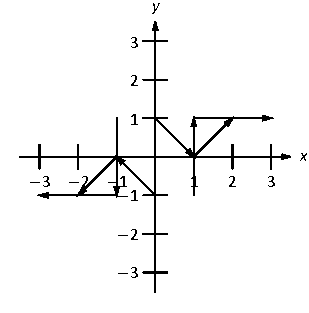
\includegraphics[width=0.43\textwidth]{fig_double_25a}}
\qquad
\subfigure[\label{fig_double_25b}]{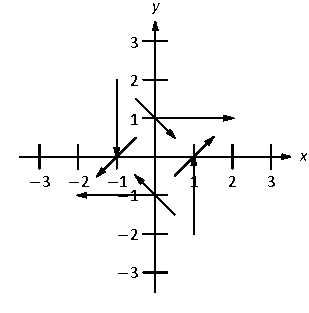
\includegraphics[width=0.43\textwidth]{fig_double_25b} }\\
\subfigure[\label{fig_double_25c}]{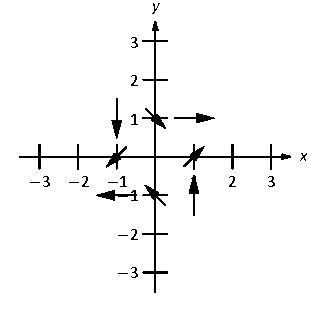
\includegraphics[width=0.43\textwidth]{fig_double_25c}}
\qquad
\subfigure[\label{fig_double_25d}]{\includegraphics[width=0.43\textwidth]{fig_double_25d} }
\caption{Demonstrating methods of graphing vector fields.}
\end{figure}
\fi

\ifpython
A common way to address this problem is limit the length of each arrow, and represent long vectors with thick arrows, as done in Figure \ref{fig_double_25c}. Usually we do not use a graph of a vector field to determine exactly the magnitude of a particular vector. Rather, we are more concerned with the relative magnitudes of vectors: which are bigger than others? Thus limiting the length of the vectors is not problematic. Python obviously allows us to plot many vectors in a vector field nicely; in Figure \ref{fig_double_25d}, we see the same vector field drawn with using the Python command \lstinline{quiver}, and finally get a clear picture of how this vector field behaves. If this vector field represented the velocity of air moving across a flat surface, we could see that the air tends to move either to the upper--right or lower--left, and moves very slowly near the origin.  We can similarly plot vector fields in space, though the plots get very busy very quickly.


\begin{figure}[h]
\centering
%\raisebox{0.5cm}{
\subfigure[\label{fig_double_25a}]{\includegraphics[width=0.43\textwidth]{fig_double_25a}}
\qquad
\subfigure[\label{fig_double_25b}]{\includegraphics[width=0.43\textwidth]{fig_double_25b} }\\
\subfigure[\label{fig_double_25c}]{\includegraphics[width=0.43\textwidth]{fig_double_25c}}
\qquad
\subfigure[\label{fig_double_25d}]{\includegraphics[width=0.43\textwidth]{fig_double_25d} }
\caption{Demonstrating methods of graphing vector fields.}
\end{figure}
\fi

\subsection{The del operator}
Often, we will drop the of $x$, $y$ and $z$ portions of the notation in Definition~\ref{def:vector_field} and refer to vector fields in the plane and in space as 
$$\vec F = \left( M, N\right) \quad \text{and} \quad \vec F  = \left( M,N,P\right),$$ respectively, as this shorthand is quite convenient.

Another item of notation will become useful: the del operator. \index{del operator}Recall in Section \ref{sec:directional_derivative} how we used the symbol $\vec{\nabla}$  to represent the gradient of a function of two variables. We now define $\vec{\nabla}$ to be the del operator. It is a vector whose components are partial derivative operations. 

In the plane, 
$$\ds\vec{\nabla} = \left( \frac{\partial}{\partial x}, \frac{\partial}{\partial y}\right);$$
in space, 
$$\ds\vec{\nabla} = \left( \frac{\partial}{\partial x}, \frac{\partial}{\partial y},\frac{\partial}{\partial z}\right).$$ 

With this definition of $\vec{\nabla}$, we can better understand the gradient $\vec{\nabla} f$. As $f$ returns a scalar, the properties of scalar and vector multiplication gives
$$\vec{\nabla} f = \left( \frac{\partial}{\partial x}, \frac{\partial}{\partial y}\right) f = \left( \frac{\partial}{\partial x}\,f, \frac{\partial}{\partial y}\,f\right) = \left( f_x, f_y\right).$$

Now apply the del operator $\vec{\nabla}$ to vector fields. Let $\vec F = \left( x+\sin(y),y^2+z,x^2\right)$. We can use vector operations and find the dot product of $\vec{\nabla}$ and $\vec F$:
\allowdisplaybreaks
\begin{align*}
\vec{\nabla} \cdot \vec F &=\left( \frac{\partial}{\partial x}, \frac{\partial}{\partial y},\frac{\partial}{\partial z}\right)\cdot  \left( x+\sin(y),y^2+z,x^2\right) \\
  &= \frac{\partial}{\partial x}\left(x+\sin(y)\right)+ \frac{\partial}{\partial y}\left(y^2+z\right) + \frac{\partial}{\partial z}\left(x^2\right) \\
		&=1+2y.
\end{align*}

We can also compute their cross products:
\allowdisplaybreaks
\begin{align*}
{\vec{\nabla}\times \vec F }&= {\left( \frac{\partial}{\partial y}\left(x^2\right)-\frac{\partial}{\partial z}\left(y^2+z\right),\frac{\partial}{\partial z}\left(x+\sin(y)\right)-\frac{\partial}{\partial x}\left(x^2\right),\frac{\partial}{\partial x}\left(y^2+z\right)-\frac{\partial}{\partial y}\left(x+\sin (y)\right)\right) }\\
			&=\left( -1,-2x,-\cos(y)\right).
\end{align*}\normalsize

As we next learn about properties of vector fields, we will see how these dot and cross products with the del operator are quite useful.

\subsection{Divergence and curl}
	\checkoddpage
\marginpar{\ifoddpage\hspace*{-1.5cm}\else\hspace*{0.25cm}\fi\includegraphics[width=0.075\textwidth]{youtube}\\
\ifoddpage\hspace*{-1.75cm}\else\hspace*{0.1cm}\fi
\qrcode[height=1.75cm]{https://youtu.be/c0MR-vWiUPU}
%\includegraphics[width=0.1\textwidth]{divergence}
}
Two properties of vector fields will prove themselves to be very important: divergence and curl. Each is a special ``derivative'' of a vector field; that is, each measures an instantaneous rate of change of a vector field.

If the vector field represents the velocity of a fluid or gas, then the divergence of the field is a measure of the compressibility of the fluid. If the divergence is negative at a point, it means that the fluid is compressing: more fluid is going into the point than is going out. If the divergence is positive, it means the fluid is expanding: more fluid is going out at that point than going in. A divergence of zero means the same amount of fluid is going in as is going out. If the divergence is zero at all points, we say the field is incompressible.

It turns out that the proper measure of divergence is simply $\vec{\nabla} \cdot \vec F$, as stated in the following definition.

\begin{definition}[Divergence]\label{def:divergence}
The \textbf{divergence of a vector field $\vec F$} (\textit{divergentie van een vectorveld}) is\index{divergence}\index[aut]{divergent}
$$\divv \vec F = \vec{\nabla} \cdot \vec F.$$
\begin{itemize}
	\item In the plane, with $\vec F = \left( M,N\right)$: \  $\divv \vec F = M_x+N_y$.
	\item In space, with $\vec F = \left( M,N,P\right)$: \  $\divv \vec F = M_x+N_y+P_z$.
\end{itemize}
\end{definition}

Curl is a measure of the spinning action of the field. Let $\vec F$ represent the flow of water over a flat surface. If a small round cork were held in place at a point in the water, would the water cause the cork to spin? No spin corresponds to zero curl; counterclockwise spin corresponds to positive curl and clockwise spin corresponds to negative curl. 

In space, things are a bit more complicated. Again let $\vec F$ represent the flow of water, and imagine suspending a tennis ball in one location in this flow. The water may cause the ball to spin along an axis. If so, the curl of the vector field is a vector (not a scalar, as before), parallel to the axis of rotation, following a right hand rule: when the thumb of one's right hand points in the direction of the curl, the ball will spin in the direction of the curling fingers of the hand.

In space, it turns out the proper measure of curl is $\vec{\nabla} \times \vec F$, as stated in the following definition. To find the curl of a planar vector field $\vec F = \left( M,N\right)$, embed it into space as $\vec F = \left( M, N, 0\right)$ and apply the cross product definition. Since $M$ and $N$ are functions of just $x$ and $y$ (and not $z$), all partial derivatives with respect to $z$ become 0 and the result is simply $\left( 0,0,N_x-M_y\right)$. The third component is the measure of curl of a planar vector field. 

\begin{definition}[Curl]\label{def:curl}
\begin{itemize}
	\item Let $\vec F = \left( M,N\right)$ be a vector field in the plane. The \textbf{curl of $\vec F$} (\textit{rotatie of rotor van $\vec F$}) is $$\curl \vec F = N_x - M_y.$$\index{curl}\index[aut]{rotatie}
	\item Let $\vec F = \left( M,N,P\right)$ be a vector field in space. The \textbf{curl of $\vec F$} (\textit{rotatie of rotor van $\vec F$}) is $$\curl \vec F = \vec{\nabla} \times \vec F = \left( P_y-N_z,\,M_z-P_x,\,N_x - M_y\right).$$
\end{itemize}
\end{definition}

We adopt the convention of referring to curl as $\vec{\nabla} \times \vec F$, regardless of whether $\vec F$ is a vector field in two or three dimensions. 

We now practice computing these quantities.

\begin{example}\label{ex_vectorfield1}
For each of the planar vector fields given below, view its graph and try to visually determine if its divergence and curl are 0. Then compute the divergence and curl.

\begin{multicols}{2}
\begin{enumerate}
	\item $\vec F = \left( y,0\right)$\quad  (see Figure \ref{fig_double_26a})
	\item $\vec F = \left( -y,x\right)$ \quad  (see Figure \ref{fig_double_26b})
	\item $\vec F = \left( x,y\right)$ \quad  (see Figure \ref{fig_double_26c})
	\item $\vec F = \left( \cos(y), \sin(x)\right)$ \quad  (see Figure \ref{fig_double_26d})
\end{enumerate}
\end{multicols}

\begin{figure}[H]
\centering
%\raisebox{0.5cm}{
\subfigure[\label{fig_double_26a}]{\includegraphics[width=0.4\textwidth]{fig_double_26a}}
\qquad
\subfigure[\label{fig_double_26b}]{\includegraphics[width=0.4\textwidth]{fig_double_26b} }\\
\subfigure[\label{fig_double_26c}]{\includegraphics[width=0.4\textwidth]{fig_double_26c}}
\qquad
\subfigure[\label{fig_double_26d}]{\includegraphics[width=0.4\textwidth]{fig_double_26d} }
\caption{The vector fields in parts 1 (a), 2 (b), 3 (c) and 4 (d) in Example \ref{ex_vectorfield1}.}
\end{figure}


\xhrulefill{gray}{2.5pt}Solution \xhrulefill{gray}{2.5pt}


\begin{enumerate}
	\item The arrow sizes are constant along any horizontal line, so if one were to draw a small box anywhere on the graph, it would seem that the same amount of fluid would enter the box as exit. Therefore it seems the divergence is zero; it is, as 
	$$\divv\vec F = \vec{\nabla} \cdot \vec F = M_x + N_y = \frac{\partial}{\partial x}(y) + \frac{\partial}{\partial y}(0) = 0.$$

	At any point on the $x$-axis, arrows above it move to the right and arrows below it move to the left, indicating that a cork placed on the axis would spin clockwise. A cork placed anywhere above the $x$-axis would have water above it moving to the right faster than the water below it, also creating a clockwise spin. A clockwise spin also appears to be created at points below the $x$-axis. Thus it seems the curl should be negative (and not zero). Indeed, it is:
	$$\curl \vec F = \vec{\nabla}\times\vec F = N_x-M_y = \frac{\partial}{\partial x}(0) - \frac{\partial}{\partial y}(y) = -1.$$
	
	\item It appears that all vectors that lie on a circle of radius $r$, centered at the  origin, have the same length (and indeed this is true). That implies that the divergence should be zero: draw any box on the graph, and any fluid coming in will lie along a circle that takes the same amount of fluid out. Indeed, the divergence is zero, as
	$$\divv\vec F = \vec{\nabla} \cdot \vec F = M_x + N_y = \frac{\partial}{\partial x}(-y) + \frac{\partial}{\partial y}(x) = 0.$$
	
		Clearly this field moves objects in a circle, but would it induce a cork to spin? It appears that yes, it would: place a cork anywhere in the flow, and the point of the cork closest to the origin would feel less flow than the point on the cork farthest from the origin, which would induce a counterclockwise flow. Indeed, the curl is positive:
	$$\curl \vec F = \vec{\nabla}\times\vec F = N_x-M_y = \frac{\partial}{\partial x}(x) - \frac{\partial}{\partial y}(-y) = 1-(-1) = 2.$$
	Since the curl is constant, we conclude the induced spin is the same no matter where one is in this field.
	
	\item At the origin, there are many arrows pointing out but no arrows pointing in. We conclude that at the origin, the divergence must be positive (and not zero). If one were to draw a box anywhere in the field, the edges farther from the origin would have larger arrows passing through them than the edges close to the origin, indicating that more is going from a point than going in. This indicates a positive (and not zero) divergence. This is correct:
	$$\divv\vec F = \vec{\nabla} \cdot \vec F = M_x + N_y = \frac{\partial}{\partial x}(x) + \frac{\partial}{\partial y}(y) = 1+1=2.$$
	
	One may find this curl to be harder to determine visually than previous examples. One might note that any arrow that induces a clockwise spin on a cork will have an equally sized arrow inducing a counterclockwise spin on the other side, indicating no spin and no curl. This is correct, as
	$$\curl \vec F = \vec{\nabla}\times\vec F = N_x-M_y = \frac{\partial}{\partial x}(y) - \frac{\partial}{\partial y}(x) = 0.$$
	

	\item	One might find this divergence hard to determine visually as large arrows appear in close proximity to small arrows, each pointing in different directions. Instead of trying to rationalize a guess, we compute the divergence:
	$$\divv\vec F = \vec{\nabla} \cdot \vec F = M_x + N_y = \frac{\partial}{\partial x}\left(\cos(y)\right) + \frac{\partial}{\partial y}\left(\sin(x)\right) = 0.$$ 
	Perhaps surprisingly, the divergence is 0.
	
	With all the loops of different directions in the field, one is apt to reason the curl is variable. Indeed, it is:
	$$\curl \vec F = \vec{\nabla}\times\vec F = N_x-M_y = \frac{\partial}{\partial x}\left(\sin(x)\right) - \frac{\partial}{\partial y}\left(\cos(y)\right) = \cos(x) + \sin(y).$$
	Depending on the values of $x$ and $y$, the curl may be positive, negative, or zero.
\end{enumerate}



\end{example}


\begin{example}\label{ex_vectorfield3}
The force of gravity between two objects is inversely proportional to the square of the distance between the objects. Locate a point mass at the origin. Create a vector field $\vec F$ that represents the gravitational pull of the point mass at any point $(x,y,z)$. Find the divergence and curl of this field. 


\xhrulefill{gray}{2.5pt}Solution \xhrulefill{gray}{2.5pt}

The point mass pulls toward the origin, so at $(x,y,z)$, the force will pull in the direction of $\left( -x, -y, -z\right)$. To get the proper magnitude, it will be useful to find the unit vector in this direction. Dividing by its magnitude, we have $$\vec u = \left( \frac{-x}{\sqrt{x^2+y^2+z^2}}, \frac{-y}{\sqrt{x^2+y^2+z^2}},\frac{-z}{\sqrt{x^2+y^2+z^2}}\right).$$
The magnitude of the force is inversely proportional to the square of the distance between the two points. Letting $k$ be the constant of proportionality, we have the magnitude as $$\ds\frac{k}{x^2+y^2+z^2}.$$ Multiplying this magnitude by the unit vector above, we have the desired vector field:
$$\vec F = \left( \frac{-kx}{(x^2+y^2+z^2)^{3/2}}, \frac{-ky}{(x^2+y^2+z^2)^{3/2}},\frac{-kz}{(x^2+y^2+z^2)^{3/2}}\right).$$
We leave it to the reader to confirm that $\divv \vec F = 0$ and $\curl \vec F = \vec 0$.

The analogous planar vector field is given in Figure \ref{fig_double_27}. Note how all arrows point to the origin, and the magnitude gets very small when far from the origin.

\begin{figure}[H]
	\begin{center}
			\includegraphics[width=0.5\textwidth]{fig_double_27}
	\caption{A vector field representing a planar gravitational force.}
	\label{fig_double_27}
	\end{center}
\end{figure}

\end{example}




A function $z=f(x,y)$ naturally induces a vector field, $\vec F = \vec{\nabla} f = \left( f_x,f_y\right)$. Given what we learned of the gradient in Section \ref{sec:directional_derivative}, we know that the vectors of $\vec F$ point in the direction of greatest increase of $f$. Because of this, $f$ is said to be the \textbf{potential function of} $\vec F$. Vector fields that are the gradient of potential functions will play an important role in the remainder of this  section.

The last part of this section applies calculus to vector fields. A common application is this: let $\vec F$ be a vector field representing a force (hence it is called a force field) and let a particle move along a curve $C$ under the influence of this force. What work is performed by the field on this particle? The solution lies in correctly applying the concepts of line integrals in the context of vector fields.


\section{Line Integrals over vector fields}\label{sec:line_int_vf}
\subsection{Definition}
Suppose a particle moves along a curve $C$ under the influence of an electromagnetic force described by a vector field $\vec F$. Since a force is inducing motion, work is performed. How can we calculate how much work is performed?

Recall that when moving in a straight line, if $\vec F$ represents a constant force and $\vec d$ represents the direction and length of travel, then work is simply $W = \vec F\cdot \vec d$. However, we generally want to be able to calculate work even if $\vec F$ is not constant and $C$ is not a straight line.

As we have practised many times before, we can calculate work by first approximating, then refining our approximation through a limit that leads to integration. 

Assume as we did at the beginning of this section, $C$ can be parametrized by the arc length parameter $s$. Over a short piece of the curve with length $ds$, the curve is approximately straight and our force is approximately constant. The straight--line direction of this short length of curve is given by $\vec T$, the unit tangent vector;   let $\vec d = \vec T\,ds$, which gives  the direction and magnitude of a small section of $C$. Thus work over this small section of $C$ is $\vec F \cdot \vec d = \vec F\cdot \vec T\, ds$. 

Summing up all the work over these small segments gives an approximation of the work performed. By taking the limit as $ds$ goes to zero, and hence the number of segments approaches infinity, we can obtain the exact amount of work. Hence, we see that 
$$W = \int_C \vec F\cdot \vec T\,ds,$$
is a line integral.

This line integral is beautiful in its simplicity, yet is not so useful in making actual computations (largely because the arc length parameter is so difficult to work with). To compute actual work, we need to parametrize $C$ with another parameter $t$ via a vector--valued function $\vec r(t)$. Since $ds = \norm{\vrp(t)}\,dt$ and $\vec T = \vrp(t)/\norm{\vrp(t)}$, we get
\begin{equation}
W = \int_C \vec F\cdot\vec T\ ds = \int_C \vec F\cdot \frac{\vrp(t)}{\norm{\vrp(t)}}\ \norm{\vrp(t)}\ dt = \int_C\vec F\cdot \vrp(t)\ dt = \int_C \vec F\cdot d\vec r,
\label{eq:line_integral}\end{equation}
where the final integral uses the differential $d\vec r$ for $\vrp(t)\,dt$.

These integrals are known as line integrals over vector fields. By contrast, the line integrals we dealt with earlier are sometimes referred to as line integrals over scalar fields. Just as a vector field is defined by a function that returns a vector, a scalar field is a function that returns a scalar, such as $z = f(x,y)$.

We formally define this line integral, then give examples and applications.

\begin{definition}[Line integral over a vector field]\label{def:line_integral2}
Let $\vec F$ be a vector field with continuous components defined on a smooth curve $C$, parametrized by $\vrt$, and let $\vec T$ be the unit tangent vector of $\vrt$. The \textbf{line integral over $\vec F$} along $C$ is\index{line integral}
$$\int_C \vec F\cdot d\vec r = \int_C \vec F\cdot\vec T\ ds.$$
\end{definition}

In Definition \ref{def:line_integral2}, note how the dot product $\vec F \cdot \vec T$ is just a scalar. 
Therefore, this new line integral is really just a special kind of line integral. Indeed, letting $f(s) = \vec F(s)\cdot \vec T(s)$, the right--hand side simply becomes $\int_C f(s)\ ds$, and we can use the corresponding techniques to evaluate the integral. This is summarized in the following theorem. 

\begin{theorem}[Evaluating a line integral over a vector field]\label{idea:line2}
Let $\vec F$ be a vector field with continuous components defined on a smooth curve $C$, parametrized by $\vrt$, $a\leq t\leq b$, where $\vec r$ is continuously differentiable. Then\index{vector field!over vector field}
	$$\int_C\vec F\cdot\vec T\ ds = \int_C \vec F\cdot d\vec r =\int\limits_a^b \vec F\big(\vec r(t)\big) \cdot \vrp(t)\ dt.$$
\end{theorem}

This theorem indicates that we can use any continuously differentiable parametrization $\vrt$ of $C$ that preserves the orientation of $C$: there isn't a right one. In practice, choose one that seems easy to work with. 

Note that the above definition and theorem implicitly evaluate $\vec F$ along the curve $C$, which is parametrized by $\vrt$. For instance, if $\vec F = \left( x+y, x-y\right)$ and $\vrt = \left( t^2,\cos(t)\right)$, then evaluating $\vec F$ along $C$ means substituting the $x$- and $y$-components of $\vrt$ in for $x$ and $y$, respectively, in $\vec F$. Therefore, along $C$, $\vec F = \left( x+y,x-y\right) = \left( t^2+\cos(t), t^2-\cos(t)\right)$. Since we are substituting the output of $\vrt$ for the input of $\vec F$, we write this as $\vec F\big(\vrt\big)$. This is a slight abuse of notation as technically the input of $\vec F$ is to be a point, not a vector, but this shorthand is useful.


\begin{example}\label{ex_livf1}
Two particles move from $(0,0)$ to $(1,1)$ under the influence of the force field $\vec F  = \left( x, x+y\right)$. One particle follows $C_1$, the line $y=x$; the other follows $C_2$, the curve $y=x^4$, as shown in Figure \ref{fig_double_28}. Force is measured in Newtons and distance is measured in meters. Find the work performed by each particle.


\begin{figure}[H]
	\begin{center}
			\includegraphics[width=0.5\textwidth]{fig_double_28}
	\caption{Paths through a vector field in Example \ref{ex_livf1}.}
	\label{fig_double_28}
	\end{center}
\end{figure}


\xhrulefill{gray}{2.5pt}Solution \xhrulefill{gray}{2.5pt}

To compute work, we need to parametrize each path. We use $\vec r_1(t) = \left( t,t\right)$ to parametrize $y=x$, and let $\vec r_2(t) =\left( t,t^4\right)$ parametrize $y=x^4$; for each, $0\leq t\leq 1$. 

Along the straight--line path, $\vec F\big(\vec r_1(t)\big) = \left( x, x+y\right) = \left( t, t+t\right) = \left( t,2t\right)$. We find $\vrp_1(t) =\left( 1,1\right)$. The integral that computes work is:
\begin{align*}
\int_{C_1} \vec F\cdot d\vec r &= \int\limits_0^1 \left( t,2t\right)\cdot\left( 1,1\right)\ dt \\
			&= \int\limits_0^1 3t\ dt \\
			&= \left(\frac32t^2\right)\Bigg|_0^1 = 1.5 \text{ joules}.
\end{align*}

Along the curve $y = x^4$, we have that
$$\vec F\big(\vec r_2(t)\big) = \left( x, x+y\right) = \left( t, t+t^4\right).$$ We find $\vrp_2(t) = \left( 1, 4t^3\right)$. The work performed along this path is
\begin{align*}
\int_{C_2} \vec F\cdot d\vec r &= \int\limits_0^1 \left( t,t+t^4\right)\cdot\left( 1,4t^3\right)\ dt\\
			&= \int\limits_0^1 \big(t + 4t^4+ 4t^7\big)\ dt \\
			&= \left(\frac12t^2 + \frac45t^5 + \frac12t^8\right)\Bigg|_0^1 =  1.8 \text{ joules}.
\end{align*}


Note how differing amounts of work are performed along the different paths. This should not be too surprising: the force is variable, one path is longer than the other, etc.
\end{example}

\begin{example}\label{ex_livf2}
Two particles move from $(-1,1)$ to $(1,1)$ under the influence of a force field $\vec F = \left( y, x\right)$. One moves along the curve $C_1$, the parabola defined by $y = 2x^2-1$. The other particle moves along the curve $C_2$, the bottom half of the circle defined by $x^2+(y-1)^2=1$, as shown in Figure \ref{fig_double_29}. Force is measured in Newton and distances are measured in meters. Find the work performed by moving each particle along its path.

\begin{figure}[H]
	\begin{center}
			\includegraphics[width=0.5\textwidth]{fig_double_29}
	\caption{Paths through a vector field in Example \ref{ex_livf2}.}
	\label{fig_double_29}
	\end{center}
\end{figure}


\xhrulefill{gray}{2.5pt}Solution \xhrulefill{gray}{2.5pt}

We start by parametrizing $C_1$: the parametrization $\vec r_1(t) = \left( t, 2t^2-1\right)$ is straightforward, giving $\vrp_1 = \left( 1,4t\right)$. On $C_1$, $\vec F\big(\vec r_1(t)\big) = \left( y,x\right) = \left( 2t^2-1,t\right)$.


Computing the work along $C_1$, we have:
\begin{align*}
\int_{C_1} \vec F\cdot d\vec r_1 & = \int\limits_{-1}^1 \left( 2t^2-1,t\right)\cdot\left( 1,4t\right)\ dt \\
		&= \int\limits_{-1}^1 \big(2t^2-1+4t^2\big)\ dt = 2 \text{ joules}.
\end{align*}





For $C_2$, it is probably simplest to parametrize the half circle using sine and cosine. Recall that $\vec r(t) = \left( \cos(t), \sin(t)\right)$ is a parametrization of the unit circle on $0\leq t\leq 2\pi$; we add 1 to the second component to shift the circle up one unit, then restrict the domain to $\pi\leq t\leq 2\pi$  to obtain only the lower half, giving $\vec r_2(t) = \left( \cos(t), \sin(t)+1\right)$, $\pi\leq t\leq 2\pi$, and hence $\vrp_2(t) = \left( -\sin(t), \cos(t)\right)$ and $\vec F\big(\vec r_2(t)\big) = \left(y,x\right) = \left( \sin(t)+1,\cos(t)\right)$.


Computing the work along $C_2$, we have:
\begin{align*}
\int_{C_2} \vec F\cdot d\vec r_2 & = \int\limits_{\pi}^{2\pi} \left( \sin(t)+1,\cos(t)\right)\cdot\left( -\sin(t),\cos(t)\right)\ dt \\
		&= \int\limits_{\pi}^{2\pi} \big(-\sin^2(t)-\sin(t)+\cos^2(t)\big)\ dt = 2 \text{ joules}.
\end{align*}
Note how the work along $C_1$ and $C_2$ in this example is the same. 
\end{example}

\subsection{Properties}
Line integrals over vector fields share the same properties as line integrals over scalar fields, with one important distinction. The orientation of the curve $C$ matters with line integrals over vector fields, whereas it did not matter with line integrals over scalar fields.

It is relatively easy to see why. Let $C$ be the unit circle. The area under a surface over $C$ is the same whether we traverse the circle in a clockwise or counterclockwise fashion, hence the line integral over a scalar field on $C$ is the same irrespective of orientation. On the other hand, if we are computing work done by a force field, direction of travel definitely matters. Opposite directions create opposite signs when computing dot products, so traversing the circle in opposite directions will create line integrals that differ by a factor of $-1$. 

In summary, we have the following properties of line integrals over vector fields. 

\begin{enumerate}
	\item	Let $\vec F$ and $\vec G$ be  vector fields with continuous components defined on a smooth curve $C$, parametrized by $\vrt$, and let $k_1$ and $k_2$ be scalars. Then\index{line integral!properties over a vector field}
	$$\ds \int_C\big(k_1\vec F+k_2\vec G\big)\cdot d\vec r = k_1\int_C\vec F\cdot d\vec r +k_2\int_C\vec G\cdot d\vec r.$$
	\item Let $C$ be piecewise smooth, composed of smooth components $C_1$ and $C_2$. Then
	$$\int_C\vec F\cdot d\vec r = \int_{C_1}\vec F\cdot d\vec r + \int_{C_2}\vec F\cdot d\vec r.$$
	\item	Let $C^*$ be the curve $C$ with opposite orientation, parametrized by $\vec r^*$. Then
	$$\int_C\vec F\cdot d\vec r = -\int_{C^*}\vec F\cdot d\vec r^*.$$
	\end{enumerate}

We demonstrate using these properties in the following example.

\begin{example}\label{ex_livf3}
Let $\vec F = \left( 3(y-1/2),1\right)$ and let $C$ be the path that starts at $(0,0)$, goes to $(1,1)$ along the curve $y=x^3$, then returns to $(0,0)$ along the line $y=x$, as shown in Figure \ref{fig_double_30}. Evaluate $\oint_C \vec F\cdot d\vec r$.


\begin{figure}[H]
	\begin{center}
			\includegraphics[width=0.5\textwidth]{fig_double_30}
	\caption{The vector field and curve in Example \ref{ex_livf3}.}
	\label{fig_double_30}
	\end{center}
\end{figure}


\xhrulefill{gray}{2.5pt}Solution \xhrulefill{gray}{2.5pt}

As $C$ is piecewise smooth, we break it into two components $C_1$ and $C_2$, where $C_1$ follows the curve $y=x^3$ and $C_2$ follows the curve $y=x$. 

We parametrize $C_1$ with $\vec r_1(t) = \left( t, t^3\right)$ on $0\leq t\leq 1$, with $\vrp_1(t) = \left( 1,3t^2\right)$. We will use \linebreak $\vec F\big(\vec r_1(t)\big) = \left( 3(t^3-1/2),1\right)$.

While we always have unlimited ways in which to parametrize a curve, there are two direct methods to choose from when parametrizing $C_2$. The parametrization $\vec r_2(t)=\left( t,t\right)$, $0\leq t\leq 1$ traces the correct line segment but with the wrong orientation. Relying on property (3) of line integrals over vector fields, we can use this parametrization and negate the result.

Another choice is to use the techniques of Section \ref{sec:lines} to create the line with the orientation we desire. We wish to start at $( 1,1)$ and travel in the $\vec d = \left( -1,-1\right)$ direction for one length of $\vec d$, giving equation $\vec \ell(t) = \left( 1,1\right) + t\left( -1,-1\right) = \left( 1-t,1-t\right)$ on $0\leq t\leq 1$.

Either choice is fine; we choose $\vec r_2(t)$ to practice using line integral properties. We find \linebreak $\vrp_2(t) = \left( 1,1\right)$ and $\vec F\big(\vec r_2(t)\big) = \left( 3(t-1/2),1\right)$.

Evaluating the line integral:
\begin{align*}
\oint_C \vec F\cdot d\vec r &= \int_{C_1}\vec F\cdot d\vec r_1 - \int_{C_2}\vec F\cdot d\vec r_2 \\
			&= \int\limits_0^1 \left( 3\left(t^3-\dfrac{1}{2}\right),1\right)\cdot \left( 1,3t^2\right) dt- \int\limits_0^1 \left( 3\left(t-\dfrac{1}{2}\right),1\right)\cdot \left(1,1\right) dt \\
			&= \int\limits_0^1\left(3t^3+3t^2-\dfrac{3}{2}\right)\ dt - \int\limits_0^1 \left(3t-\dfrac{1}{2}\right)\ dt\\
			&= \dfrac{1}{4} - 1 = -\dfrac{3}{4}.
\end{align*}
If we interpret this integral as computing work, the negative work implies that the motion is mostly against the direction of the force, which seems plausible when we look at Figure \ref{fig_double_30}.
\end{example}

\subsection{The fundamental theorem of line integrals}
	\checkoddpage
\marginpar{\ifoddpage\hspace*{-1.5cm}\else\hspace*{0.25cm}\fi\includegraphics[width=0.075\textwidth]{youtube}\\
\ifoddpage\hspace*{-1.75cm}\else\hspace*{0.1cm}\fi
\qrcode[height=1.75cm]{https://youtu.be/6S3BJSsc72Q}
%\includegraphics[width=0.1\textwidth]{regions}
}

We are preparing to make important statements about the value of certain line integrals over special vector fields. Before we can do that, we need to define some terms that describe the domains over which a vector field is defined.

A region in the plane is \textbf{connected}\index{connected}\index[aut]{samenhangend} (\textit{samenhangend}) if any two points in the region can be joined by a piecewise smooth curve that lies entirely in the region. In Figure \ref{fig_double_31a}, sets $R_1$ and $R_2$ are connected; set $R_3$ is not connected, though it is composed of two connected subregions.

A region is \textbf{simply connected} (\textit{enkelvoudig samenhangend})\index{simply connected}\index{connected!simply}\index[aut]{samenhangend ! enkelvoudig} if every simple closed curve that lies entirely in the region can be continuously deformed (shrunk) to a single point without leaving the region.  (A curve is \textbf{simple}\index{simple curve} if it does not cross itself.) In Figure \ref{fig_double_31a}, only set $R_1$ is simply connected. Region $R_2$ is not simply connected as any closed curve that goes around the ``hole'' in $R_2$ cannot be continously shrunk to a single point. As $R_3$ is not even connected, it cannot be simply connected, though again it consists of two simply connected subregions. 

We have applied these terms to regions of the plane, but they can be extended intuitively to domains in space (and hyperspace). In Figure \ref{fig_double_31b}, the domain bounded by the sphere (at left) and the domain with a subsphere removed (at right) are both simply connected. Any simple closed path that lies entirely within these domains can be continuously deformed into a single point. In Figure \ref{fig_double_31c}, neither domain is simply connected. At left, the ball has a hole that extends its length and the pictured closed path cannot be deformed to a point. At right, two paths are illustrated on the torus that cannot be shrunk to a point. 

We will use the terms connected and simply connected in subsequent definitions and theorems.

\begin{figure}
\centering
%\raisebox{0.5cm}{
\subfigure[\label{fig_double_31a}]{\includegraphics[width=0.43\textwidth]{fig_double_31a}}
\qquad
\subfigure[\label{fig_double_31b}]{\includegraphics[width=0.43\textwidth]{fig_double_31b} }\\

\subfigure[\label{fig_double_31c}]{\includegraphics[width=0.43\textwidth]{fig_double_31c}}
\caption{Different types of regions (a): $R_1$ is simply connected; $R_2$ is connected, but not simply connected; $R_3$ is not connected; simply connected domains (b) and not simply connected domains in (c).}
\end{figure}

Recall how in Example \ref{ex_livf2} particles moved from $A = (-1,1)$ to $B = (1,1)$ along two different paths, wherein the same amount of work was performed along each path. It turns out that regardless of the choice of path from $A$ to $B$, the amount of work performed under the field $\vec F = \left( y, x\right)$ is the same. Since our expectation is that differing amounts of work are performed along different paths, we give such special fields a name. 

\pagebreak
\begin{definition}[Conservative field]\label{def:conservative}
Let $\vec F$ be a vector field defined on an open, connected domain $D$ containing points $A$ and $B$. If the line integral
$\int_C \vec F\cdot d\vec r$\ \ has the same value for all choices of paths $C$ starting at $A$ and ending at $B$, and parametrized by $\vec{r}(t)$,  then\index{conservative field}\index{vector field!conservative}\index{path independent}\index{line integral!path independent}\index[aut]{vectorveld!conservatief}\index[aut]{vectorveld!exact}\index[aut]{conservatief vectorveld}
\begin{itemize}
	\item $\vec F$ is a \textbf{conservative field} (\textit{conservatief vectorveld}) and
	\item	The line integral $\int_C \vec F\cdot d\vec r$ is path independent and can be written as $$\int_C \vec F\cdot d\vec r = \int\limits_A^B \vec F\cdot \ d\vec r.$$ 
\end{itemize}
\end{definition}


How can we tell if a field is conservative? To show a field $\vec F$ is conservative using the definition, we need to show that all line integrals from points $A$ to $B$ have the same value. It is equivalent to show that all line integrals over closed paths $C$ are 0. Each of these tasks are generally nontrivial.

There is, however, a simpler method. Consider the surface defined by $z = f(x,y) = xy$. We can compute the gradient of this function: $\vec{\nabla} f = \left( f_x, f_y\right) = \left( y, x\right)$. Note that this is the field from Example \ref{ex_livf2}, which we have claimed is conservative. We will soon give a theorem that states that a field $\vec F$ is conservative if, and only if, it is the gradient of some scalar function $f$. To show $\vec F$ is conservative, we need to determine whether or not $\vec F = \vec{\nabla} f$ for some function $f$. To recognize the special relationship between $\vec F$ and $f$ in this situation, $f$ is given a name.

\begin{definition}[Potential function]\label{def:potential}
Let $f$ be a differentiable function defined on a  domain $D$  (e.g., $z = f(x,y)$ or $w = f(x,y,z)$) and let $\vec F = \vec{\nabla} f$, the gradient of $f$. Then $f$ is a \textbf{potential function} (\textit{potentiaalfunctie}) of $\vec F$.\index{potential function}\index{vector field!potential function}\index[aut]{vectorveld!potentiaalfunctie}\index[aut]{potentiaalfunctie}
\end{definition}

We now state the fundamental theorem of line integrals, also known as the gradient theorem, which connects conservative fields and path independence to fields with potential functions. 

\begin{theorem}[Fundamental theorem of line integrals]\label{thm:FTofLineIntegrals}
Let $\vec F$ be a vector field whose components are continuous on a connected domain $D$, let $A$ and $B$ be any points in $D$, and let $C$ be any path in $D$ starting at $A$ at $t=a$,  ending at $B$ at $t=b$ and parametrized by $\vec{r}(t)$ such that $\vec{r}(a)=A$ and  $\vec{r}(b)=B$. 
\begin{enumerate}
	\item $\vec F$ is conservative if and only if there exists a differentiable function $f$ such that $\vec F = \vec{\nabla} f$. 
	\item	If $\vec F$ is conservative, then 
	$$\int_C\vec F\cdot d\vec r = \int\limits_A^B \vec F\cdot d\vec r =f\left( {\vec r\left( b \right)} \right) - f\left( {\vec r\left( a \right)} \right)= f(B) - f(A).$$
\end{enumerate}
\end{theorem}

Note that we did not specify the number of variables for the function since it is really immaterial to the theorem. The theorem will hold regardless of the number of variables in the function.


\ifanalysis
For the purpose of the proof we will assume that we are working in three dimensions, but it can be done in any dimension. Let us then start by just computing the line integral.
\begin{align*}
\int_C{{\vec{\nabla} f\cdot d\vec r}} & = \int\limits_{{\,a}}^{{\,b}}{{\vec{\nabla} f\left( {\vec r\left( t \right)} \right)\cdot \vec r'\left( t \right)\,dt}}\\ &  = \int\limits_{{\,a}}^{{\,b}}{{\left( {\frac{{\partial f}}{{\partial x}}\frac{{dx}}{{dt}} + \frac{{\partial f}}{{\partial y}}\frac{{dy}}{{dt}} + \frac{{\partial f}}{{\partial z}}\frac{{dz}}{{dt}}} \right)\,dt}}
\end{align*}

Now, at this point we can use the chain rule to simplify the integrand as follows,
\begin{align*}\int_C{{\vec{\nabla} f\cdot d\vec r}} & = \int\limits_{{\,a}}^{{\,b}}{{\left( {\frac{{\partial f}}{{\partial x}}\frac{{dx}}{{dt}} + \frac{{\partial f}}{{\partial y}}\frac{{dy}}{{dt}} + \frac{{\partial f}}{{\partial z}}\frac{{dz}}{{dt}}} \right)\,dt}}\\ &  = \int\limits_{{\,a}}^{{\,b}}{{\frac{d}{{dt}}\left[ {f\left( {\vec r\left( t \right)} \right)} \right]\,dt}}
\end{align*}

To finish this off we just need to use the fundamental theorem of calculus for single integrals.
$$
\int_C{{\vec{\nabla} f\cdot d\vec r}} = f\left( {\vec r\left( b \right)} \right) - f\left( {\vec r\left( a \right)} \right)=f(B)-f(A)
$$
%Bron: 
%http://tutorial.math.lamar.edu/Classes/CalcIII/FundThmLineIntegrals.aspx
\fi

Once again considering Example \ref{ex_livf2}, we have $A = (-1,1)$, $B = (1,1)$ and $\vec F = \left( y,x\right)$. In that example, we evaluated two line integrals from $A$ to $B$ and found the value of each was 2. Note that $f(x,y) = xy$ is a potential function for $\vec F$. Following the fundamental theorem of line integrals, consider $f(B) - f(A)$:
$$f(B) - f(A) = f(1,1) - f(-1,1) = 1 - (-1) = 2,$$
the same value given by the line integrals.


We practice using this theorem again in the next example.

\begin{example}\label{ex_livf5}
Let $\vec F = \left( 3x^2y+2x, x^3+1\right)$, $A = (0,1)$ and $B = (1,4)$. Use the first part of the fundamental theorem of line integrals to show that $\vec F$ is conservative, then choose any path from $A$ to $B$ and confirm the second part of the theorem.

\xhrulefill{gray}{2.5pt}Solution \xhrulefill{gray}{2.5pt}


To show $\vec F$ is conservative, we need to find $z = f(x,y)$ such that $\vec F = \vec{\nabla} f = \left( f_x, f_y\right)$. That is, we need to find $f$ such that $f_x = 3x^2y+2x$ and $f_y = x^3+1$. As all we know about $f$ are its partial derivatives, we recover $f$ by integration:
$$\int\limits \frac{\partial f}{\partial x}\ dx = f(x,y) + K_1(y).$$
Note how the constant of integration $K_1(y)$ is more than just a constant: it is anything that acts as a constant when taking a derivative with respect to $x$. Any function that is a function of $y$ (containing no $x$'s) acts as a constant when deriving with respect to $x$.

Integrating $f_x$ in this example gives:
$$\int\limits \frac{\partial f}{\partial x}\ dx = \int\limits (3x^2y+2x)\ dx = x^3y+x^2 + K_1(y).$$

Likewise, integrating $f_y$ with respect to $y$ gives:
$$\int\limits \frac{\partial f}{\partial y}\ dy = \int\limits( x^3+1)\ dy = x^3y+ y + K_2(x).$$

These two results should be equal with appropriate choices of $K_2(x)$ and $K_1(y)$:
$$x^3y+x^2 + K_1(y) = x^3y+ y + K_2(x)\quad \Rightarrow\quad K_2(x) = x^2 \quad \text{and}\quad K_1(y) = y.$$

We find $f(x,y) = x^3y+x^2+y$, a potential function of $\vec F$. 

By the fundamental theorem of line integrals, regardless of the path from $A$ to $B$, 
\begin{align*}
\int\limits_A^B\vec F\cdot d\vec r &= f(B) - f(A) \\[-0.3cm]
			&= f(1,4) - f(0,1) \\
			&= 9 - 1 = 8.
\end{align*}
To illustrate the validity of the Fundamental Theorem, we pick a path from $A$ to $B$. The line between these two points would be simple to construct; we choose a slightly more complicated path by choosing the parabola $y = x^2+2x+1$. This leads to the parametrization $\vrt = \left( t, t^2+2t+1\right)$, $0\leq t\leq 1$, with $\vrp(t) = \left( 1, 2t+2\right)$. Thus
\begin{align*}
\int_C \vec F\cdot d\vec r &= \int_C\vec F\big(\vrt\big)\cdot\vrp(t)\ dt\\
				&= \int\limits_0^1\left( 3t^2(t^2+2t+1)+2t, t^3+1\right)\cdot\left( 1,2t+2\right)\ dt\\
				&= \int\limits_0^1 \left(5t^4+8t^3+3t^2+4t+2\right)\ dt\\
				&= \left(t^5+2t^4+t^3+2t^2+2t\right)\Big|_0^1\\
				&= 8,
\end{align*}				
which matches our previous result.
\end{example}

The fundamental theorem of line integrals states that we can determine whether or not $\vec F$ is conservative by determining whether or not $\vec F$ has a potential function. This can be difficult. A simpler method exists if the domain of $\vec F$ is simply connected, which is a reasonable requirement. We state this simpler method as a theorem.


\begin{theorem}[Curl of conservative fields]\label{thm:conservative_field_curl}
Let $\vec F$ be a vector field whose components are continuous on a simply connected domain $D$ in the plane or in space. Then $\vec F$ is conservative if and only if $\curl \vec F = 0$ or $\vec 0$, respectively.
\end{theorem}

In Example \ref{ex_livf5}, we showed that $\vec F =\left( 3x^2y+2x,x^3+1\right)$ is conservative by finding a potential function for $\vec F$. Using the above theorem, we can show that $\vec F(M,N)$ is conservative much more easily by computing its curl:
$$\curl \vec F = N_x - M_y = 3x^2 - 3x^2 = 0.$$



\newpage

\renewcommand{\ExerciseListName}{Assignement}
\section{Exercises}

\subsection*{\nameref{sec:iterated_integrals}}
%%%%%%%%%%%%%%%%
%Oefening 1
%%%%%%%%%%%%%%%%
\begin{Exercise} Evaluate the given double integrals.
    \begin{multicols}{2}
       \Question[difficulty = 1] $\ds \int\limits_0^2\int\limits_{x}^{2x} \left(x^2+y^2\right)\ dy\ dx$
       \Question[difficulty = 1] $\ds \int\limits_1^2\int\limits_{y}^{y^3} e^{\frac{x}{y}}\ dx\ dy$
        \Question[difficulty = 1] $\ds \int\limits_1^2\int\limits_{y}^{3y} (x+y)\ dx\ dy$
        \Question[difficulty = 2] $\ds \int\limits_{-1}^2\int\limits_{2x^2-2}^{x^2+x} x\ dy\ dx$
        \Question[difficulty = 2] $\ds \int\limits_{0}^{\pi}\int\limits_{0}^{\cos(\theta)} r \sin(\theta)\ dr\ d\theta$
        \Question[difficulty = 1] $\ds \int\limits_{0}^{\frac{\pi}{2}}\int\limits_{2}^{4\cos(\theta)} r^3\ dr\ d\theta$
        \Question[difficulty = 2] $\ds \int\limits_{0}^1\int\limits_{0}^{1} \dfrac{x^2}{1+y^2}\ dy\ dx$
        \Question[difficulty = 2] $\ds \int\limits_{-1}^{2} \int\limits_0^1 (xy^2 + x^2y)\ dx\ dy$ 
        \Question[difficulty = 2] $\ds \int\limits_0^1\int\limits_{x^2}^{2-x^2} \sqrt{x}y\ dy\ dx$ 
        \Question[difficulty = 3] $\ds \int\limits_0^{\pi/4}\ \int\limits_{\sin(x)}^{\cos(x)} xy \ dy\ dx$ 
        \Question[difficulty = 3] $\ds \int\limits_0^{1}\ \int\limits_{\sqrt[3]{y}}^{1} e^{x^2} \ dx\ dy$
        \EndCurrentQuestion
    \end{multicols}
\end{Exercise}

\setboolean{firstanswerofthechapter}{true}
\begin{Answer}
    \begin{multicols}{2}
    
            \Question $\ds \int\limits_0^2\int\limits_{x}^{2x} \left(x^2+y^2\right)\ dy\ dx = \dfrac{40}{3}$
            \Question $\ds \int\limits_1^2\int\limits_{y}^{y^3} e^{\frac{x}{y}}\ dx\ dy = \dfrac{e}{2} (e^3-4)$
            \Question $\ds \int\limits_1^2\int\limits_{y}^{3y} (x+y)\ dx\ dy = 14$
            \Question $\ds \int\limits_{-1}^2\int\limits_{2x^2-2}^{x^2+x} x\ dy\ dx = \dfrac{9}{4}$
            \Question $\ds \int\limits_{0}^{\pi}\int\limits_{0}^{\cos(\theta)} r \sin(\theta)\ dr\ d\theta = \dfrac{1}{3}$
            \Question $\ds \int\limits_{0}^{\frac{\pi}{2}}\int\limits_{2}^{4\cos(\theta)} r^3\ dr\ d\theta = 10 \pi$
            \Question $\ds \int\limits_{0}^1\int\limits_{0}^{1} \dfrac{x^2}{1+y^2}\ dy\ dx = \dfrac{\pi}{12}$
            \Question $\ds \int\limits_{-1}^{2} \int\limits_0^1 (xy^2 + x^2y)\ dx\ dy = 2$ 
            \Question $\ds \int\limits_0^1\int\limits_{x^2}^{2-x^2} \sqrt{x}y\ dy\ dx = \dfrac{16}{21} $ 
            \Question $\ds \int\limits_0^{\pi/4}\ \int\limits_{\sin(x)}^{\cos(x)} xy \ dy\ dx = \dfrac{\pi - 2}{16}$ 
            \Question $\ds \int\limits_0^{1}\ \int\limits_{\sqrt[3]{y}}^{1} e^{x^2} \ dx\ dy = \int\limits_0^{1}\ \int\limits_0^{x^3} e^{x^2} \ dy\ dx = \dfrac{1}{2}$
    \EndCurrentQuestion
    \end{multicols}
\end{Answer}
\setboolean{firstanswerofthechapter}{false}


%%%%%%%%%%%%%%%%
%Oefening 2
%%%%%%%%%%%%%%%%
\begin{Exercise} Find the integration boundaries for the given double integrals and evaluate.
        \Question[difficulty = 1] $\ds \iint_R x^2 y \ dA$ \quad with $R$ the triangle $OAB$ with $A(3,0)$ and $B(3,2)$. %Uit Van Hecke H3, vb 3.1
        \Question[difficulty = 3] $\ds \iint_R\ dA$ \quad  with $R$ the region in the first quadrant between $y^2=x^3$ and $y=x$
        \Question[difficulty = 3] $\ds \iint_R x^2 \ dA$ \quad with $R$ the region in the first quadrant between $xy=16$, $y=x$, $y=0$ and $x=8$
        \Question[difficulty = 2] $\ds \iint_R y\ dA$\quad  with $R$ the region enclosed by $y=x^2$ and $y=x^3$
        \Question[difficulty = 3] $\ds \iint_R \dfrac{1}{\sqrt{2y-y^2}} \ dA$ \quad with $R$ the region enclosed by $x^2=4-2y$ in the first quadrant
        \Question[difficulty = 2] $\ds \iint_R e^{\frac{x}{y}} \ dA$ \quad  with $R$ the region bounded by $y^2=x$, $x=0$ en $y=1$ 
        \Question[difficulty = 3] $\ds \iint_R (y-x) \ dA$ \quad with $R$ the region enclosed by $(x-1)^2+y^2=1$
\end{Exercise}

\begin{Answer}
    
    
        \Question $\ds \iint_R x^2 y \ dA = \ds \int\limits_{0}^3\int\limits_{0}^{\frac{2}{3}x} x^2 y \ dy\ dx = \ds \int\limits_{0}^2\int\limits_{\frac{3}{2}y}^{3} x^2 y  \ dx\ dy  = \dfrac{54}{5}$
        %Uit Van Hecke H3, vb 3.1
    
         \Question $\ds \iint_R\ dA = \ds \int\limits_{0}^1\int\limits_{\sqrt{x^3}}^{x} \ dy\ dx = \ds \int\limits_{0}^1\int\limits_{y}^{\sqrt[3]{x^2}} \ dx\ dy  = \dfrac{1}{10}$
        
        \Question $\ds \iint_R x^2 \ dA =  \ds \int\limits_{0}^4\int\limits_{0}^{x} x^2 \ dy\ dx + \ds \int\limits_{4}^8\int\limits_{0}^{\frac{16}{x}} x^2 \ dy\ dx  = \ds \int\limits_{0}^2\int\limits_{y}^{8}x^2  \ dx\ dy +  \ds \int\limits_{2}^4\int\limits_{y}^{\frac{16}{y}}x^2  \ dx\ dy  = 448$ 
        
         \Question $\ds \iint_R y\ dA = \ds \int\limits_{0}^1\int\limits_{x^3}^{x^2} y\ dy\ dx = \ds \int\limits_{0}^1\int\limits_{\sqrt{y}}^{\sqrt[3]{y}} y\ dx\ dy  = \dfrac{1}{35}$ 
         
        \Question $\ds \iint_R \dfrac{1}{\sqrt{2y-y^2}} \ dA  = \ds \int\limits_{0}^2\int\limits_{0}^{\frac{4-x^2}{2}} \dfrac{1}{\sqrt{2y-y^2}}\ dy\ dx = \ds \int\limits_{0}^2\int\limits_{0}^{\sqrt{4-2y}} \dfrac{1}{\sqrt{2y-y^2}}\ dx\ dy  = 4 $ 
    
       \Question $\ds \iint_R e^{\frac{x}{y}} \ dA = \ds\int\limits_{0}^1\int\limits_{\sqrt{x}}^1 e^{\frac{x}{y}}\ dy\ dx = \ds\int\limits_{0}^1\int\limits_{0}^{y^2} e^{\frac{x}{y}}\ dx\ dy = \dfrac{1}{2}$ 
    
        \Question $\ds \iint_R (y-x) \ dA = \ds\int\limits_{-\frac{\pi}{2}}^{\frac{\pi}{2}}\int\limits_{0}^{2\cos(\theta)} r^2(\sin(\theta)-\cos(\theta))\ dr\ d\theta = -\pi$    
    
\end{Answer} 

\pagebreak
%%%%%%%%%%%%%%%%
%Oefening 3
%%%%%%%%%%%%%%%%
\begin{Exercise} Reverse the order of integration  in the integrals below.
    \begin{multicols}{2}
         \Question[difficulty = 1] $\ds \int\limits_{0}^3\int\limits_{1}^{\sqrt{4-y}} f(x,y)\ dx\ dy$
         \Question[difficulty = 2] $\ds \int\limits_{0}^1\int\limits_{\arccos(y)}^{\frac{\pi}{2}} f(x,y)\ dx\ dy$
         \Question[difficulty = 3] $\ds \int\limits_{-6}^2\int\limits_{\frac{x^2}{4}}^{3-x} f(x,y)\ dy\ dx$
         \EndCurrentQuestion
    \end{multicols}
\end{Exercise}

\begin{Answer}
    
         \Question $\ds \int\limits_{0}^3\int\limits_{1}^{\sqrt{4-y}} f(x,y)\ dx\ dy = \ds \int\limits_{1}^2\int\limits_{0}^{4-x^2} f(x,y)\ dy\ dx$
         \Question $\ds \int\limits_{0}^1\int\limits_{\arccos(y)}^{\frac{\pi}{2}} f(x,y)\ dx\ dy = \ds \int\limits_{0}^{\frac{\pi}{2}}\int\limits_{\cos(x)}^{1} f(x,y)\ dy\ dx$
         \Question $\ds \int\limits_{-6}^2\int\limits_{\frac{x^2}{4}}^{3-x} f(x,y)\ dy\ dx = \ds \int\limits_{0}^1\int\limits_{-2\sqrt{y}}^{2\sqrt{y}} f(x,y)\ dx\ dy + \ds \int\limits_{1}^9\int\limits_{-2\sqrt{y}}^{3-y} f(x,y)\ dx\ dy$
        
    
\end{Answer}
    
%%%%%%%%%%%%%%%%
%Oefening 4
%%%%%%%%%%%%%%%%    
\begin{Exercise} Using a double integral, find the area of the following regions.
        \Question[difficulty = 1] the region bounded by $y^2=10x+25$ and $y^2 = -6x+9$
        \Question[difficulty = 1] the region bounded by $y=x^3$, $x+y=2$ and the $x$-axis
        \Question[difficulty = 3] the region bounded by $x^2+y^2=2x$, $x^2+y^2 = 4x$, $y=x$ and $y=0$
        \Question[difficulty = 2] the region bounded by $r\cos (\theta) = 1$ and $r=2$ (area that does not contain $r = 0$)
        \Question[difficulty = 3] region bounded by $r= 1 +\cos (\theta)$ and $r=\cos (\theta)$ 
\end{Exercise}

\begin{Answer}
    
        \Question $A = 2 \ds 2\int\limits_{0}^{\sqrt{15}}\int\limits_{\frac{25-y^2}{-10}}^{\frac{y^2-9}{-6}} \ dx\ dy = \dfrac{16 \sqrt{15}}{3}$
        
        \Question $A = \ds \int\limits_{0}^{1}\int\limits_{y^{\frac{1}{3}}}^{2-y} \ dx\ dy =\ds \int\limits_{0}^{1}\int\limits_{0}^{x^3} \ dy\ dx + \ds \int\limits_{1}^{2}\int\limits_{0}^{2-x} \ dy\ dx  = \dfrac{3}{4}$
    
        \Question $A = \ds \int\limits_{1}^{2}\int\limits_{\sqrt{1-(x-1)^2}}^{x} \ dy\ dx + \ds \int\limits_{2}^{4}\int\limits_{0}^{\sqrt{4-(x-2)^2}} \ dy\ dx = 
        \ds \int\limits_{0}^{1}\int\limits_{1+\sqrt{1-y^2}}^{2+\sqrt{4-y^2}} \ dx\ dy + \ds \int\limits_{1}^{2}\int\limits_{y}^{2+\sqrt{4-y^2}} \ dx\ dy $ \\[0.2cm]
        $= \ds \int \limits_0^{\frac{\pi}{4}} \int\limits_{2 \cos(\theta)}^{4\cos(\theta)} \ r \ dr \ d\theta= \dfrac{3 \pi }{4} + \dfrac{3}{2} $
        
        \Question $A = 2 \ds \int\limits_{0}^{\frac{\pi}{3}}\int\limits_{\frac{1}{\cos (\theta)}}^{2} r\ dr\ d\theta = \dfrac{4 \pi }{3} - \sqrt{3}$
        
        \Question $A = 2 \ds \int\limits_{0}^{\pi}\int\limits_{0}^{1 + \cos(\theta)} r\ dr\ d\theta - 2 \ds \int\limits_{0}^{\frac{\pi}{2}}\int\limits_{0}^{\cos(\theta)} r\ dr\ d\theta = \dfrac{5 \pi }{4}$
    
\end{Answer}    


\subsection*{\nameref{sec:double_int_volume}}    
%Volume in cart coord
%%%%%%%%%%%%%%%%
%Oefening 5 
%%%%%%%%%%%%%%%%
\begin{Exercise} Find the volume of the given regions  using Cartesian coordinates.
        \Question[difficulty = 1] the region enclosed by $x=0$, $x=4$, $y=0$, $y=4$, $z=0$ en $xy=4z$
        \Question[difficulty = 2] the region enclosed by the three coordinate planes, together with the planes \\ $x^2+4y^2=4$ and $y^2+2z=4$
        \Question[difficulty = 3] the region enclosed by the three coordinate planes, together with the planes \\ $z=1-x^2-y^2$ en $x+y \leq 1$
        \Question[difficulty = 3] the region enclosed by the planes $y=x^2$, $x=y^2$, $z=0$ en $z=12 + y - x^2$
        \Question[difficulty = 3] the region formed by a truncated prism with upright side faces $x=0$, $x=2$, $y=0$, $y=1$, as ground plane $z=0$ and as upper plane $-x+y+2z=4$ 
        \Question[difficulty = 2] the region enclosed by $x^2+y^2=1$ and $x^2+z^2=1$ 
\end{Exercise}

\begin{Answer}
    
        \Question $V = \ds \int\limits_0^4 \ds \int\limits_0^{4} \dfrac{xy}{4} \ dy \ dx = 16$
       \Question $V = \ds \int\limits_0^2 \ds \int\limits_0^{\frac{\sqrt{4-x^2}}{2}} \dfrac{4-y^2}{2} \ dy \ dx   = \ds \int\limits_0^1 \ds \int\limits_0^{2\sqrt{1-y^2}} \dfrac{4-y^2}{2} \ dx\ dy = \dfrac{15 \pi}{16}$
        \Question $V =\ds \int\limits_0^1 \ds \int\limits_0^{1-x} (1-x^2-y^2) \ dy \ dx= \ds \int\limits_0^1 \ds \int\limits_0^{1-y} (1-x^2-y^2) \ dx \ dy = \dfrac{1}{3}$
        \Question $V = \ds \int\limits_0^1 \ds \int\limits_{x^2}^{\sqrt{x}} (12+y-x^2) \ dy \ dx=  \ds \int\limits_0^1\ds \int\limits_{y^2}^{\sqrt{y}} (12+y-x^2) \ dx \ dy = \dfrac{569}{140}$
  
        \Question $V = \ds \int\limits_0^2 \ds \int\limits_{0}^{1} \dfrac{4+x-y}{2} \ dy\  dx=  \ds \int\limits_0^1\ds \int\limits_{0}^{2} \dfrac{4+x-y}{2}  \ dx\  dy = \dfrac{9}{2} $
        
        \Question $V = 8 \ds \int\limits_0^1 \ds \int\limits_{0}^{\sqrt{1-x^2}} \sqrt{1-x^2} \ dy\  dx = 8 \ds \int\limits_0^1\ds \int\limits_{0}^{\sqrt{1-y^2}} \sqrt{1-x^2}  \ dx\  dy = \dfrac{16}{3} $
         
    
\end{Answer}   

%%%%%%%%%%%%%%%%
%Oefening 5 bis %Uit Van Hecke H11 oef 11 (a,b)
%%%%%%%%%%%%%%%%
\begin{Exercise} Set up the double integral to find the volume of the given region in Cartesian coordinates and in polar coordinates.
    \Question[difficulty = 1] the region enclosed by $z=0$, $z=x+y+2$ and $x^2+y^2=16$ in the first quadrant
    \Question[difficulty = 2] the region enclosed by $z=0$, $z=2xy$, $x^2+y^2+x=0$, $x < 0$ and $y<0$
\end{Exercise}

\begin{Answer}
     
        \Question $\ds \int\limits_0^4\ds \int\limits_{0}^{\sqrt{16-x^2}} (x+y+2)  \ dy\  dx = \ds \int\limits_0^{\frac{\pi}{2}} \ds \int\limits_0^{4} (r \cos(\theta) + r \sin(\theta) + 2 )\, r \ dr \ d\theta$ 
     
        \Question $\ds \int\limits_{-1}^0\ds \int\limits_{-\sqrt{-x^2-x}}^{0} 2xy \ dy\  dx = \ds \int\limits_{\pi}^{\frac{3\pi}{2}} \ds \int\limits_0^{-\cos(\theta)} 2r^3 \cos(\theta) \sin(\theta)\, \ dr \ d\theta$ 
       
    
\end{Answer}

%%%%%%%%%%%%%%%%
%Oefening 6
%%%%%%%%%%%%%%%%
\begin{Exercise} Find the volume of the given region using polar coordinates.
    \Question[difficulty = 2] the region enclosed by $x^2+y^2=2$, $z=0$ and $z=2$ and where $z\geq x^2+y^2$
    \Question[difficulty = 2] the region enclosed by $x^2+y^2=2$, $z=0$ and $z=2$ and where $z\leq x^2+y^2$
     \Question[difficulty = 2] the region enclosed by $x^2+y^2=1$, cut off by $x^2+y^2+z^2=4$ 
    \Question[difficulty = 2] the region enclosed by $x^2+y^2=2z$, cut off by $x^2+y^2+z^2=3$
    \Question[difficulty = 3] the region enclosed by $x^2+y^2+z^2=a^2$ en $x^2+y^2=ax$ 
    \Question[difficulty = 3] the region enclosed by $x^2+y^2=2y$ and $z^2=y$ 
\end{Exercise}

\begin{Answer}
    
        \Question $V = \ds \int\limits_0^{2\pi} \ds \int\limits_0^{\sqrt{2}} \left(2-r^2\right) r \ dr \ d\theta = 2\pi$
        
        \Question $V = \ds \int\limits_0^{2\pi} \ds \int\limits_0^{\sqrt{2}} r^3 \ dr \ d\theta = 2\pi$
     
        \Question $V = 8 \ds \int\limits_0^{\frac{\pi}{2}} \ds \int\limits_0^{1} \sqrt{4 - r^2}\, r \ dr \ d\theta = \dfrac{4 \pi}{3}\left(8-3\sqrt{3}\right)$

        \Question $V = \ds \int\limits_0^{\sqrt{2}} \ds \int\limits_0^{2\pi} \left(\sqrt{3-r^2} - \dfrac{r^2}{2}  \right)\, r\ d\theta \ dr = \dfrac{\pi}{3}\left( 6\sqrt{3} - 5 \right)$

        \Question $V = 4 \ds \int\limits_0^{\frac{\pi}{2}} \ds \int\limits_0^{a\cos(\theta)} \sqrt{a^2 - r^2}\, r \ dr \ d\theta = \dfrac{4}{3}a^3 \left(- \dfrac{2}{3} + \dfrac{\pi}{2} \right)$
        
        \Question $V = 4 \ds \int\limits_0^{\frac{\pi}{2}} \ds \int\limits_0^{2\sin(\theta)} \sqrt{r \sin(\theta)}\, r \ dr \ d\theta = \dfrac{64 \sqrt{2}}{15}$
    
    
\end{Answer}

\subsection*{\nameref{sec:center_of_mass}}
%%%%%%%%%%%%%%%%
%Oefening 7 
%%%%%%%%%%%%%%%%
\begin{Exercise} Find the center of mass of the  regions below with the given mass density.
        \Question[difficulty = 1]  the flat region enclosed  by $y= \sin (x)$ and $y=0 \ (0\leq x \leq \pi)$ with mass density \\ $\delta(x,y) = ky$. 
        \Question[difficulty = 3]  the flat region enclosed by $y^2 = 4x + 4$ en $y^2 = -2x+4$ with mass density $\delta = 1$ 
        \Question[difficulty = 2]  a triangular plate enclosed by the $x$- and $y$-axis and the $2x+3y=12$ with mass density $\delta = 1$ 
\end{Exercise}

\begin{Answer}
    
        \Question  \begin{itemize}
            \item $M = \ds \int\limits_0^{\pi}\int\limits_{0}^{\sin(x)}ky \ dy\  dx = \dfrac{k \pi}{4}$ 
            \item $M_{y} = k \ds \int\limits_0^{\pi}\int\limits_{0}^{\sin(x)} xy \ dy\  dx = \dfrac{k \pi^2}{8} \quad \Rightarrow \overline{x} = \dfrac{\pi}{2}$
            \item $M_{x} = k \ds \int\limits_0^{\pi}\int\limits_{0}^{\sin(x)} y^2 \ dy\  dx = \dfrac{4 k }{9}  \quad \Rightarrow \overline{y} = \dfrac{16}{9\pi} $
        \end{itemize}
         Mass density: $\left(\dfrac{\pi}{2}, \dfrac{16}{9\pi}\right)$
        
        \Question  
        \begin{itemize}
            \item $M = 2 \ds \int\limits_0^{2} \ds \int\limits_{\frac{y^2-4}{4}}^{\frac{y^2-4}{-2}} 1 \ dx\  dy = 8$ 
            \item $M_{y} = 2 \ds \int\limits_0^{2}\int\limits_{\frac{y^2-4}{4}}^{\frac{y^2-4}{-2}} x \ dx\  dy = \dfrac{16}{5} \quad \Rightarrow \overline{x} = \dfrac{2}{5}$ 
            \item $M_{x} = 2 \ds \int\limits_0^{2}\int\limits_{\frac{y^2-4}{4}}^{\frac{y^2-4}{-2}} y \ dx\  dy = 0 \quad \Rightarrow \overline{y} = 0 $ 
        \end{itemize}
        Mass density: $\left(\dfrac{2}{5}, 0\right)$
        
        \Question  
        \begin{itemize}
            \item $M = \ds \int\limits_0^{4} \ds \int\limits_{0}^{\frac{12-3y}{2}} 1 \ dx\  dy = 12$ 
            \item $M_{y} = \ds \int\limits_0^{4} \ds \int\limits_{0}^{\frac{12-3y}{2}} x \ dx\  dy = 24 \quad \Rightarrow \overline{x} = 2$ 
            \item $M_{x} = \ds \int\limits_0^{4} \ds \int\limits_{0}^{\frac{12-3y}{2}} y \ dx\  dy = 16 \quad \Rightarrow \overline{y} = \dfrac{4}{3}$ 
        \end{itemize}
        Mass density: $\left(2,\dfrac{4}{3}\right)$
        
    
\end{Answer} 


\subsection*{\nameref{sec:surface_area}} 
%%%%%%%%%%%%%%%%
%Oefening 8
%%%%%%%%%%%%%%%%    
\begin{Exercise} Find the requested surface area.
    \Question[difficulty = 3] the part of $x^2+y^2 = 3z^2$, located above the $xy$-plane and inside $x^2+y^2=4y$
    \Question[difficulty = 2] the part of $x^2+z^2=16$, inside $x^2+y^2=16$
    \Question[difficulty = 3] the part of $z^2=4x$, inside $y^2=4x$ and $x \leq 1$
    \Question[difficulty = 3] the part of $z=1-x^2-y^2$, inside $x^2+y^2=1$
    \Question[difficulty = 2] the part of $x^2+y^2+z^2= 1$ that is cut off by $x^2+4y^2=1$.
\end{Exercise}

\begin{Answer}
    
    \Question $SA=2 \ds \int\limits_0^{\frac{\pi}{2}} \int\limits_0^{4 \sin(\theta) } \dfrac{2}{\sqrt{3}} \, r \  dr \ d\theta = \dfrac{8 \pi}{\sqrt{3}}$
    
    \Question $SA=8 \ds \int\limits_0^{4} \int\limits_0^{\sqrt{16-x^2}} \sqrt{\dfrac{16}{16-x^2}}  \  dy \ dx = 128 $
    
    \Question $SA=4 \ds \int\limits_0^{1} \int\limits_0^{2\sqrt{x}} \sqrt{\dfrac{x+1}{x}}  \  dy \ dx = \dfrac{16}{3} \left(2 \sqrt{2}-1 \right) $
    
    \Question $SA= \ds \int\limits_0^{2\pi} \int\limits_0^{1} \sqrt{1+4r^2} \ r \ dr \ d\theta = \dfrac{\pi}{6} \left(5\sqrt{5}-1 \right)$
    
    \Question $SA= 8 \ds \int\limits_0^{1} \int\limits_0^{\frac{\sqrt{1 - x^2}}{2}} \sqrt{ \dfrac{1}{1-x^2-y^2}} \ dy \ dx = \dfrac{4\pi}{3}$
    
\end{Answer}


\subsection*{\nameref{sec:line_int_intro}}
%%%%%%%%%%%%%%%%
%Oefening 9
%%%%%%%%%%%%%%%%
\begin{Exercise} Evaluate the line integral of the scalar functions below along the given curve. 
    \Question[difficulty = 2] $\ds \int\limits_C x^2 \ ds$ \quad along the intersection of $x-y+z=0$ en $x+y+2z=0$ from $(0,0,0)$ to $(3,1,-2)$ 
    \Question[difficulty = 1] $\ds \int\limits_C y \ ds$ \quad from $x=3$ to $x=24$ along the curve $C: \, y=2\sqrt{x}$
    \Question[difficulty = 3] $\ds \int\limits_C (x+y) \ ds$ \quad along the right loop of $r^2 = 2 \cos (2 \theta)$
    \Question[difficulty = 3] $\ds \int\limits_C \dfrac{ds}{x^2 + y^2 + z^2}$ \quad along the first loop of $x(t) = 8 \cos (t),\  y(t) = 8 \sin(t),\  z(t) = t$
    \Question[difficulty = 3] $\ds \int\limits_C \sqrt{2y^2 + z^2} \ ds$ \quad along the curve $$C: \,\left\{ \begin{array}{l}x^2+y^2+z^2 = 4 \\ y = x \end{array} \right.$$
    \Question[difficulty = 3] $\ds \int\limits_C e^z \ ds$ \quad along the curve \  $x(t) = e^t \cos (t),\  y(t) = e^t \sin(t), \ z(t) = t$  
     \Question[difficulty = 3] $\ds \int\limits_C \sqrt{1+4x^2z^2} \ ds$ \quad along the curve $$C: \,\left\{ \begin{array}{l}x^2+z^2 = 1 \\ y = x^2 \end{array} \right.$$ 
     \Question[difficulty = 2] $\ds \int\limits_C x \ ds$ \quad along the curve $$C: \,\left\{ \begin{array}{l}x^2+y^2 = a^2 \\ z=x \end{array} \right.$$ in the first octant 
     \Question[difficulty = 2] $\ds \int\limits_C z \ ds$ \quad along the curve $$C: \,\left\{ \begin{array}{l}x^2+y^2 +z^2= 1 \\ x+y=1 \end{array} \right.\quad \text{ met } z \geq 0$$  
\end{Exercise}

\begin{Answer}
    
    \Question $\ds \int\limits_C x^2 \ ds = 3 \sqrt{14}$
    \Question $\ds \int\limits_C y \ ds = 156$
    \Question $\ds \int\limits_C (x+y) \ ds = 2 \sqrt{2}$
    \Question $\ds \int\limits_C \dfrac{ds}{x^2 + y^2 + z^2} = \dfrac{\sqrt{65}}{8} \arctan\left(\dfrac{\pi}{4} \right)$
    \Question $\ds \int\limits_C \sqrt{2y^2 + z^2} \ ds = 8\pi$
    \Question $\ds \int\limits_C e^z \ ds = \dfrac{e^{2\pi}\sqrt{1+2e^{4\pi}} - \sqrt{3}}{2} + \dfrac{1}{2\sqrt{2}} \ln \left( \dfrac{\sqrt{2}e^{2\pi}+\sqrt{1+2e^{4\pi}}}{\sqrt{2}+\sqrt{3}} \right)$
    \Question $\ds \int\limits_C \sqrt{1+4x^2z^2} \ ds = 3 \pi$
    \Question $\ds \int\limits_C x \ ds = \dfrac{a^2}{2} \left( \sqrt{2} + \ln \left( 1 + \sqrt{2} \right) \right)$
    \Question $\ds \int\limits_C z \ ds = 1$ 
    
\end{Answer}    


\subsection*{\nameref{sec:vector_fields}}
%%%%%%%%%%%%%%%%
%Oefening 10
%%%%%%%%%%%%%%%%   
\begin{Exercise}[difficulty = 2, label = Oef_grafiek_vectorvelden] Which vector field belongs to which graph in Figure \ref{fig_double_32}?
    \begin{multicols}{2}
        \Question $\vec F_1 = \dfrac{\vec r}{\norm{\vec r}}$
        \Question $\vec F_2 = \vec r$
        \Question $\vec F_3 = y \hat{\imath} - x \hat{\jmath}$
        \Question $\vec F_4 = x \hat{\jmath}$
        \EndCurrentQuestion
    \end{multicols}
    
\begin{figure}[H]
\includegraphics[scale=0.29]{fig_double_32a} \hspace{1.5cm}
\includegraphics[scale=0.41]{fig_double_32b}
\\
\includegraphics[scale=0.4]{fig_double_32c}
\hspace{1.5cm}
\includegraphics[scale=0.4]{fig_double_32d}
\caption{Vector fields from exercise \ref{Oef_grafiek_vectorvelden} }
\label{fig_double_32}
\end{figure}

\end{Exercise}

\begin{Answer}
    \begin{multicols}{2}
    
        \Question $\vec F_1 = \dfrac{\vec r}{\norm{\vec r}} \quad \rightarrow$ graph $II$
        \Question $\vec F_2 = \vec r  \quad  \rightarrow$ graph $I$
        \Question $\vec F_3 = y \hat{\imath} - x \hat{\jmath}  \quad  \rightarrow$ graph $IV$
        \Question $\vec F_4 = x \hat{\jmath}  \quad  \rightarrow$ graph $III$
    \EndCurrentQuestion
    \end{multicols}
\end{Answer}

%%%%%%%%%%%%%%%%
%Oefening 11
%%%%%%%%%%%%%%%%  
\begin{Exercise}[difficulty = 1] Consider a scalar function $f(x,y,z)=x^2yz^3$ and a vector field $\vec F = (xz, -y^2, 2x^2y)$. Find $\vec{\nabla} f$, \, $\vec{\nabla}  \cdot \vec F$ \, and \, $\vec{\nabla} \times \vec F $.
\end{Exercise}

\begin{Answer}
    $\nabla f  = (2xyz^3, x^2 z^3, 3x^2yz^2)$, \, $\nabla  \cdot \vec F = z-2y$ \, and \, $ \nabla \times \vec F = (2x^2, -4xy+x,0)$
\end{Answer}

%%%%%%%%%%%%%%%%
%Oefening 12
%%%%%%%%%%%%%%%%     
\begin{Exercise}[difficulty = 2] Consider a scalar function $f(x,y,z)=xy+yz+xz$ and a vector field $\vec F = (x^2y, -y^2z, z^2x)$. Find $\vec{\nabla} f$, \, $\vec{\nabla}  \cdot \vec F$, \, $\vec{\nabla} \times \vec F $\, en \, $(\vec{\nabla} f) \times \vec F $\, at $(3,-1,2)$.
\end{Exercise}

\begin{Answer}

    $\nabla f  = (y+z, x+z, y+x) \quad \Rightarrow \quad \nabla f(3,-1,2)  = (1, 5, 2)$, \,    $\nabla  \cdot \vec F = 0$,\\[0.2cm] 
    $ \nabla \times \vec F = (y^2, -z^2,-x^2) \quad \Rightarrow \quad (\nabla \times \vec F)(3,-1,2) = (1,-4,-9)$\, and \\[0.2cm] $(\vec \nabla f) \times \vec F = (x^2 z^2+xz^3+y^3z+xy^2z, -xyz^2-xz^3+x^2y^2+x^3y,-y^3z-y^2z^2-x^3y-x^2yz) $ \\[0.2cm] 
    $\Rightarrow \quad ((\vec \nabla f) \times \vec F)(3,-1,2) = (64,-30,43)  $
\end{Answer}

%%%%%%%%%%%%%%%%
%Oefening 16
%%%%%%%%%%%%%%%%        
\begin{Exercise} Find all points in space where the direction of the given vector field does not change. 
    \begin{multicols}{2}
        \Question[difficulty = 2] $\vec F = (xy^2, xyz, z-2x)$
        \Question[difficulty = 3] $\vec F = (xy^3, xyz, z-x^2)$
        \EndCurrentQuestion
    \end{multicols}
\end{Exercise}

\begin{Answer}
    
        \Question The direction of the vector field changes in all points.
        \Question In points on the $y$-axis or the $z$-axis, the direction of the vector field does not change.
    
\end{Answer}

%%%%%%%%%%%%%%%%
%Oefening 17
%%%%%%%%%%%%%%%%    
\begin{Exercise}[difficulty = 3] Consider the vector field $\vec F = \left(\frac{3x}{z}, 2x, 7yz \right)$ and the curve $C$ described by  $\vec r(t) = (\cos^2(t), \sin (t), -\cos(t))$ with $0 \leq t < 2 \pi$. At which points of $C$ has the rotor of $\vec F$ a min/max length?
\end{Exercise}

\begin{Answer}

    $\nabla \times \vec F = \left(7z, -\dfrac{3x}{z^2}, 2 \right) \quad \Rightarrow$ on the curve $C$: $\nabla \times \vec F=\left( -7 \cos(t), -3, 2 \right) $ \\[0.2cm]
    The length of the rotor is maximal if $\cos(t) = \pm 1$. This corresponds to the points $(1,0, \pm 1)$ on $C$. The length of the rotor is minimal if $\cos(t) = 0$. This corresponds to the points $(0, \pm 1, 0) $ on $C$.
\end{Answer}

%%%%%%%%%%%%%%%%
%Oefening 18
%%%%%%%%%%%%%%%%
\begin{Exercise}[difficulty = 3] The coulomb potential $V$ in a vacuum at a point $P(x,y,z)$ originating from a point charge $q$ placed at the origin is given by
\[ V(x,y,z) = \dfrac{q}{4\pi\epsilon_0 \sqrt{x^2+y^2+z^2}}\,, \]
with $\epsilon_0$ a constant. Find the corresponding electric field given by $\vec E = -\vec{\nabla} V$.
\end{Exercise}

\begin{Answer}

    Imagine $\overrightarrow{OP} = (x,y,z)$ with $r=\sqrt{x^2+y^2+z^2}$, then $V = \dfrac{q}{4\pi\epsilon_0 \sqrt{x^2+y^2+z^2}}$. We then obtain that
\[ \vec E = -\nabla V = -\dfrac{q}{4\pi\epsilon_0 \left(\sqrt{x^2+y^2+z^2}\right)^3}(x,y,z) = \dfrac{q \vec r}{4\pi\epsilon_0\, r^3} \]
\end{Answer}

\pagebreak
\subsection*{\nameref{sec:line_int_vf}}
%%%%%%%%%%%%%%%%
%Oefening 13
%%%%%%%%%%%%%%%% 
\begin{Exercise} Evaluate the line integral of the given vector field along the given curve(s). 
        \Question[difficulty = 2] $\vec F = \left(\cos (x), y \right)$ \quad along $y=\sin(x)$ from $(0,0)$ to $(\pi,0)$
        \Question[difficulty = 2] $\vec F = (xy, y-x)$ \quad from $(0,0)$ to $(1,1)$ along the curves $C_1: \, y=x$, \, $C_2: \, y=x^2$ \, and \, $C_3: \, y^2=x$
        \Question[difficulty = 3] $\vec F = (2xy, x^2)$ \quad from $(0,0)$ to $(1,2)$ along the curves $C_1: \, y=2x$, \, $C_2: \, y=2x^2$, \\ $C_3: \, y^2=4x$ \, and \, $C_4: \, y=2x^3$
        \Question[difficulty = 2] $\vec F = \left(\dfrac{1}{\sqrt{xy}}, -\dfrac{1}{\sqrt{xy}} \right)$ \quad along the curve $C: \, y=1-x$ from $x=0$ to $x=1$ %Boek Ottoy, oef 1 hfdstk 20
        \Question[difficulty = 1] $\vec F = (x^2y, xy^2)$ \quad along the curve $$C: \, \left\{ \begin{array}{l} x = \dfrac{t}{2} \\ y = \sqrt{2t} \end{array} \right.$$ from $(0,0)$ to $(1,2)$ 
        \Question[difficulty = 3] $\vec F = \left(\sqrt{b^2-y^2}, \sqrt{a^2-x^2} \right)$ \quad along the curve $$C: \, \dfrac{x^2}{a^2} + \dfrac{y^2}{b^2} = 1\, $$ with \, $x\geq 0, y \geq 0$ travelled  in a counterclockwise fashion
        \Question[difficulty = 3] $\vec F = (-3y, 2x)$ \quad along the curve $C: \, abca$ with $a(1,2)$, $b(3,1)$ and $c(3,2)$
        \Question[difficulty = 2] $\vec F = \left(3x^2+2xy, x^2+y^2 \right)$ \quad from $(1,1)$ to $(2,2)$ along the curve $C_1: \, y=x$  \, and \, along the path given by $C_2: \, y=1$ \, and \, $C_3: \, x=2$
        \Question[difficulty = 3] $\vec F = (y^2, z^2, x^2)$ \quad along the curve $$C: \, \left\{ \begin{array}{l} y=1  \\ x^2 + y^2 + z^2 = 5 \end{array} \right.$$ with $x \geq 0$, travelled in the direction of increasing $z$-values
\end{Exercise}

\begin{Answer}
    
        \Question $\ds \int_C \vec F\cdot d\vec r = 0$

        \Question $\ds \int_{C_1} \vec F\cdot d\vec r = \dfrac{1}{3}, \quad \ds \int_{C_2} \vec F\cdot d\vec r = \dfrac{1}{12}, \quad \ds \int_{C_3} \vec F\cdot d\vec r = \dfrac{17}{30}$
        
        \Question $\ds \int_{C_i} \vec F\cdot d\vec r = 2\ $ for $i=1\ldots4$
        
        \Question $\ds \int_C \vec F\cdot d\vec r = 2\pi$
        \Question $\ds \int_C \vec F\cdot d\vec r = \dfrac{76}{35}$
        \Question $\ds \int_C \vec F\cdot d\vec r = 0$
        \Question $\ds \int_C \vec F\cdot d\vec r= 5$
        
        \Question $\ds \int_{C_1} \vec F\cdot d\vec r = \dfrac{49}{3}, \quad \ds \int_{C_2} \vec F\cdot d\vec r = \dfrac{49}{3}, \quad \ds \int_{C_3} \vec F\cdot d\vec r = 0$
       
        \Question $\ds \int_C \vec F\cdot d\vec r = \dfrac{32}{3}$
    
\end{Answer}


%%%%%%%%%%%%%%%%
%Oefening 14
%%%%%%%%%%%%%%%% 

\begin{Exercise}[difficulty = 3]
Do the following sets of points represent a region, a connected region or simply connected region?
    \begin{multicols}{2}
    \Question $R = \left\{ (x,y) \in \mathbb{R}^2 \left| \ x > 0, \ y \geq 0  \right. \right\}$
    \Question $R = \left\{ (x,y) \in \mathbb{R}^2 \left| \ x = 0, \ y \geq 0  \right. \right\}$
    \Question $R = \left\{ (x,y) \in \mathbb{R}^2 \left| \ x \neq 0, \ y > 0  \right. \right\}$
    \Question $R = \left\{ (x,y,z) \in \mathbb{R}^3 \left| \ x^2 > 1  \right. \right\}$
    \Question $R = \left\{ (x,y,z) \in \mathbb{R}^3 \left| \ x^2 + y^2 > 1  \right. \right\}$
    \Question $R = \left\{ (x,y,z) \in \mathbb{R}^3 \left| \ x^2 + y^2 + z^2 > 1  \right. \right\}$
    \EndCurrentQuestion
    \end{multicols}
\end{Exercise}

\begin{Answer}
    
        \Question $R = \left\{ (x,y) \in \mathbb{R}^2 \left| \ x > 0, \ y \geq 0  \right. \right\}$ is a simply connected region
        \Question $R = \left\{ (x,y) \in \mathbb{R}^2 \left| \ x = 0, \ y \geq 0  \right. \right\}$ is not a region.
        \Question $R = \left\{ (x,y) \in \mathbb{R}^2 \left| \ x \neq 0, \ y > 0  \right. \right\}$ is a region but not connected. There is no path in $R$ from $(-1,1)$ to $(1,1)$.
        \Question $R = \left\{ (x,y,z) \in \mathbb{R}^3 \left| \ x^2 > 1  \right. \right\}$ is a region but not connected. There is no path in $R$ from $(-2,0,0)$ to $(2,0,0)$.
        \Question $R = \left\{ (x,y,z) \in \mathbb{R}^3 \left| \ x^2 + y^2 > 1  \right. \right\}$ is a connected region. The circle $x^2+y^2=2, z=0$ lies in $R$, but cannot be shrunk to a point while staying the region. 
        \Question $R = \left\{ (x,y,z) \in \mathbb{R}^3 \left| \ x^2 + y^2 + z^2 > 1  \right. \right\}$ is a single coherent area.
    
\end{Answer}

%%%%%%%%%%%%%%%%
%Oefening 15
%%%%%%%%%%%%%%%%    
\begin{Exercise} Verify that the given vector field is conservative and, if possible, find a potential function.
    \begin{multicols}{2}
     \Question[difficulty = 2] $\vec F = \left(xy, \dfrac{1}{2}x^2-y^2 \right)$ 
        \Question[difficulty = 1] $\vec F = \left(y, x, -2z \right)$ 
        \Question[difficulty = 2] $\vec F = \left( \dfrac{x}{x^2+y^2}, \dfrac{y}{x^2+y^2} \right)$
        \Question[difficulty = 1] $\vec F = \left( \dfrac{x}{x^2+y^2}, -\dfrac{y}{x^2+y^2} \right)$ 
        \Question[difficulty = 1] $\vec F = \left( 2xy-z^2, 2yz+x^2, -2zx+y^2\right)$ 
        \Question[difficulty = 3] $\vec F = e^{x^2+y^2+z^2}\left( xz, yz, xy\right)$ 
        \Question[difficulty = 3] $\vec F = \left( xy - \sin (z), \dfrac{1}{2}x^2 - \dfrac{e^y}{z}, \dfrac{e^y}{z^2} - x \cos (z)\right)$ 
        \EndCurrentQuestion
\end{multicols}
\end{Exercise}

\begin{Answer}
    
     \Question $\vec F = \left(xy, \dfrac{1}{2}x^2-y^2 \right)$ is conservative. A potential function is $f(x,y) = \dfrac{x^2y}{2} - \dfrac{y^3}{3}$.
     \Question $\vec F = \left(y, x, -2z \right)$ is conservative. A potential function is $f(x,y,z) = xy - z^2$.
     \Question $\vec F = \left( \dfrac{x}{x^2+y^2}, \dfrac{y}{x^2+y^2} \right)$ is conservative. A potential function is $f(x,y) = \dfrac{\ln \left(x^2 + y^2 \right)}{2} $.
     \Question $\vec F = \left( \dfrac{x}{x^2+y^2}, -\dfrac{y}{x^2+y^2} \right)$ is not conservative. 
     \Question $\vec F = \left( 2xy-z^2, 2yz+x^2, -2zx+y^2\right)$ is conservative. A potential function is \\ $f(x,y,z) = x^2y-xz^2+y^2z$.
     \Question $\vec F = e^{x^2+y^2+z^2}\left( xz, yz, xy\right)$ is not conservative. 
     \Question $\vec F = \left( xy - \sin (z), \dfrac{1}{2}x^2 - \dfrac{e^y}{z}, \dfrac{e^y}{z^2} - x \cos (z)\right)$ is conservative. A potential function is \\ $f(x,y,z) = \dfrac{x^2y}{2} -  \dfrac{e^y}{z} - x \sin(z)$.
    
\end{Answer}






	\begin{center}
			\includegraphics[width=0.65\textwidth]{GreatMath_7.jpg}
	\end{center}
